\chapter{Case Study: a 1/2-spin XYZ Heisenberg Chain Coupled to Two External Baths}
\label{Chapter3}

\section{The Model}
We are going to consider a Heisenberg XYZ chain of N $\frac{1}{2}$-spin, coupled to two external reservoirs positioned at the boundaries of the chain. The density matrix describing the chain evolves according to the Lindblad master equation
\begin{equation}
    \frac{d\rho}{dt} = -i[H, \rho] - \sum_{a=1}^{2}\gamma_a\Bigl(\frac{1}{2}L_a^{\dagger}L_a\rho + \frac{1}{2}\rho L_a^{\dagger}L_a - L_a\rho L_a^{\dagger}\Bigl),
\end{equation}
$H$ being the Hamiltonian of the model:
\begin{equation}
\label{ham_chain}
    H = \sum_{i = 1}^{N-1} (J_x \sigma_i^x \sigma_{i+1}^x + J_y \sigma_i^y \sigma_{i+1}^y + J_z \sigma_i^z \sigma_{i+1}^z),
\end{equation}
and the $\gamma_a$ being bath-coupling strength parameters. The $L_a$ are the Lindblad operators representing the single-spin bath coupled to the first and the last spin of the chain:
\begin{equation}
\label{dissipators}
    L_1 = \frac{1}{2}(\sigma_x + i\sigma_y), \quad L_2 = \frac{1}{2}(\sigma_x - i\sigma_y).
\end{equation}

As disclosed previously, we are going to study this physical system through three numerical method: the QT method, the CSR method and the MPO method. \textcolor{red}{We will see how everyone of these methods will be useful until they reach their own limitations; examining these limits will be interesting and advantageous to set a benchmark [for numerical methods]}.

In the following sections, we will study three fundamental observables for the analysis of a XYZ Heisenberg chain: the magnetization profile, the two-point correlation function, the spin current; in particular, we will examine them in chains of different lengths: 4, 8, 12, 16 sites. 

Before we begin the analysis, a look to the convergence of the three methods for every chain length is worthwhile. In this way, we will be able to set the method parameters in order to obtain  plausible results.

%%%%%%%%%%%%%%%%%%%%%%%%%%%%%%%%%%%%%%%%%%%%%%%%%%%%%%%%%%%%%%%%%%
%%%%%%%%%%%%%%%%%%%%%%%%%%%%%%%%%%%%%%%%%%%%%%%%%%%%%%%%%%%%%%%%%%
%%%%%%%%%%%%%%%%%%%%%%%%%%%%%%%%%%%%%%%%%%%%%%%%%%%%%%%%%%%%%%%%%%
\section{The CSR Method: Limitations and Usability}
The CSR method, described in section~\ref{chapter2_csr}, would have been an important tool to study in greater detail the model previously characterized, both for confirming results coming from the other methods and for allowing us to study much longer chains. As we will see in the following section, the CSR method is not suitable for describing such a model.

In order to show this, we can easily see the case of a 4-sites chain for the proposed model. In particular, we can study the magnetization profile of the chain, i.e. the expectation value $\langle \sigma^z \rangle$ of the Pauli spin- matrix $\sigma^z$ for each site. 

\begin{figure}[H]
    \centering
    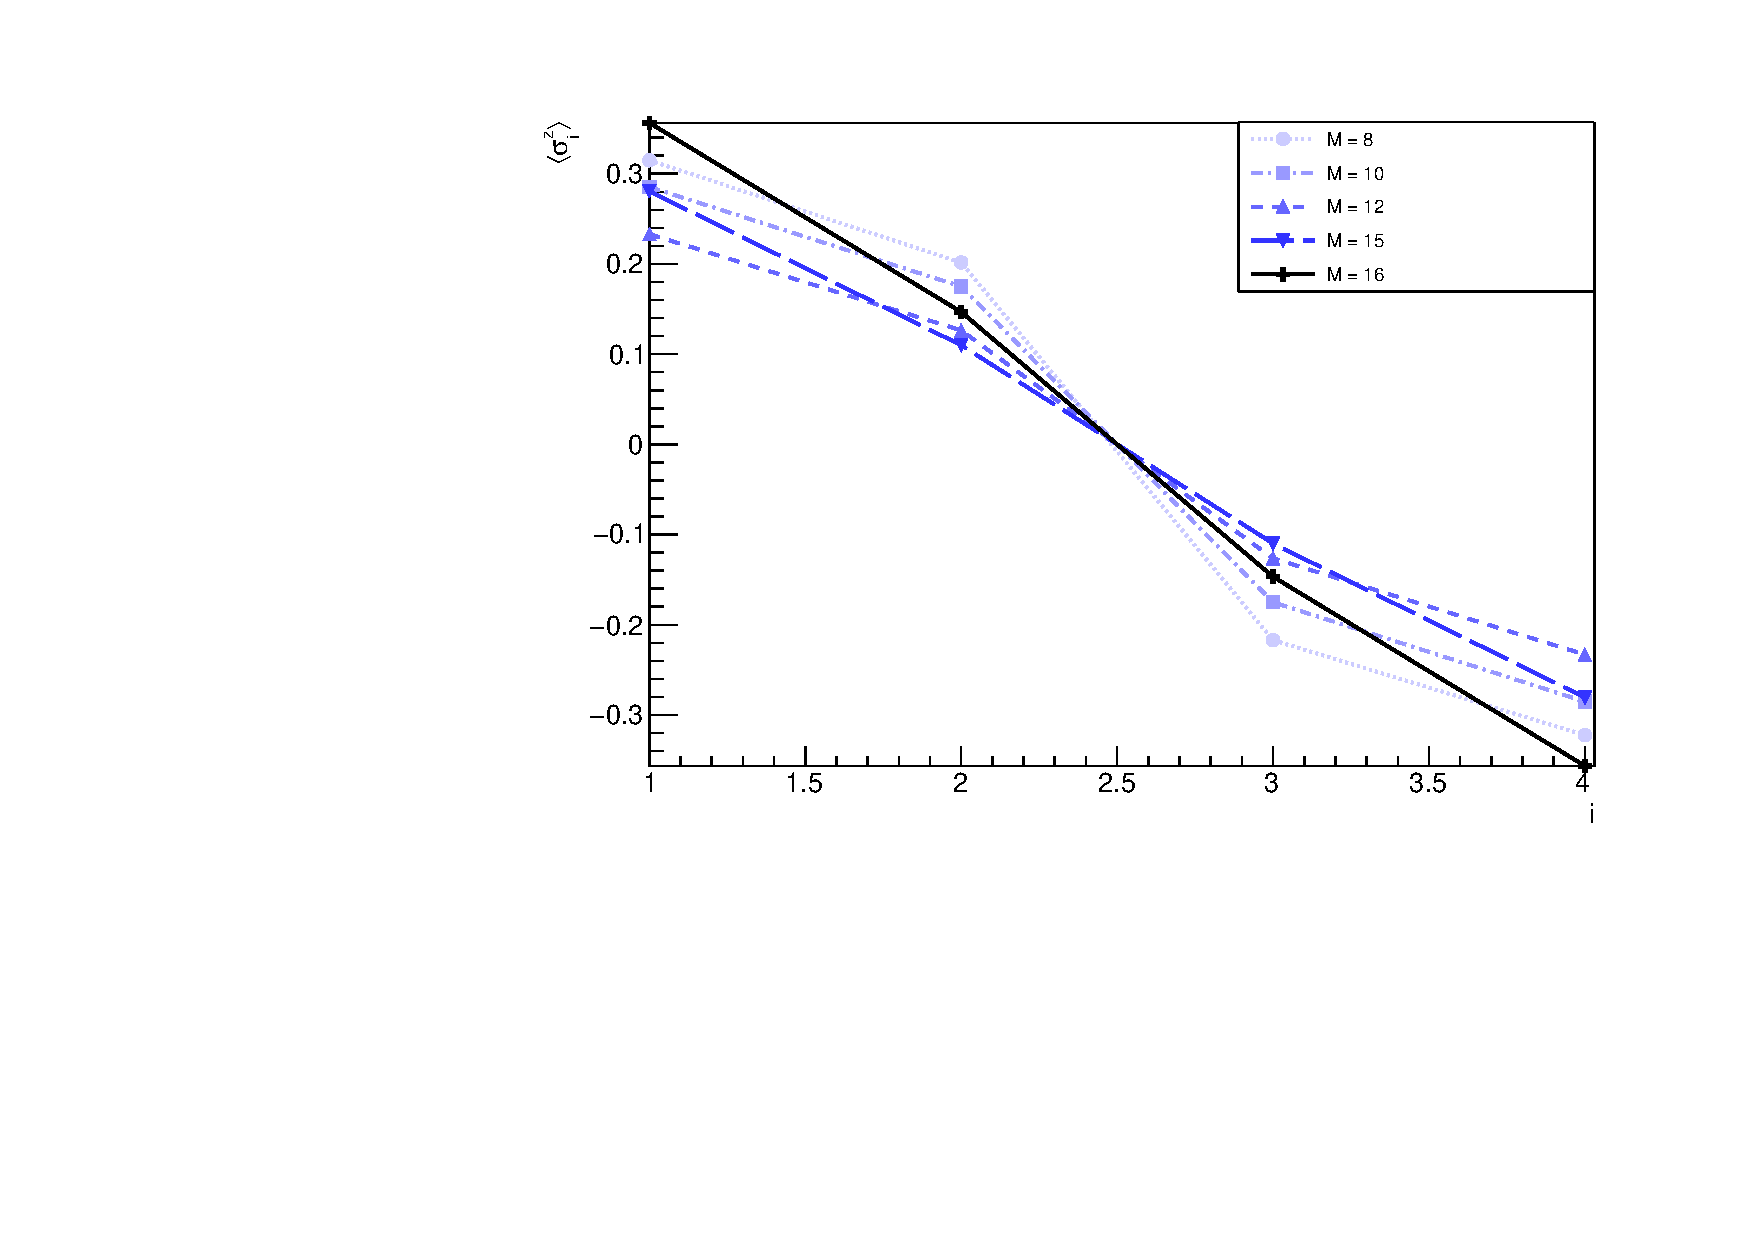
\includegraphics[scale=0.7]{Figures/4sites/4sites_LM_convergenceIncreasingM.pdf}
    \caption{Spin profile for a 4-sites chain for the model described above with $J_z=1$ for several values of corner-space dimensions $M \times M$. The cyan markers are those representing the data for the value of M covering the entire Hilbert space (of dimensions $2^4 \times 2^4$).}
    \label{fig:4sites_LM_convergenceIncreasingM}
\end{figure}

As shown in figure~\ref{fig:4sites_LM_convergenceIncreasingM}, it is clear that for such a system the convergence has not been reached. Even for $M = 15$, that covers almost the total Hilbert space dimension, the results are not the convergent ones.

On the other hand, if we consider a model in which every site is coupled to a dissipator (e.g. of the same type of the ones delineated in~\ref{dissipators}), we can see how the magnetization profile gets to convergence starting from $M = 9$ already.


\begin{figure}[H]
    \centering
    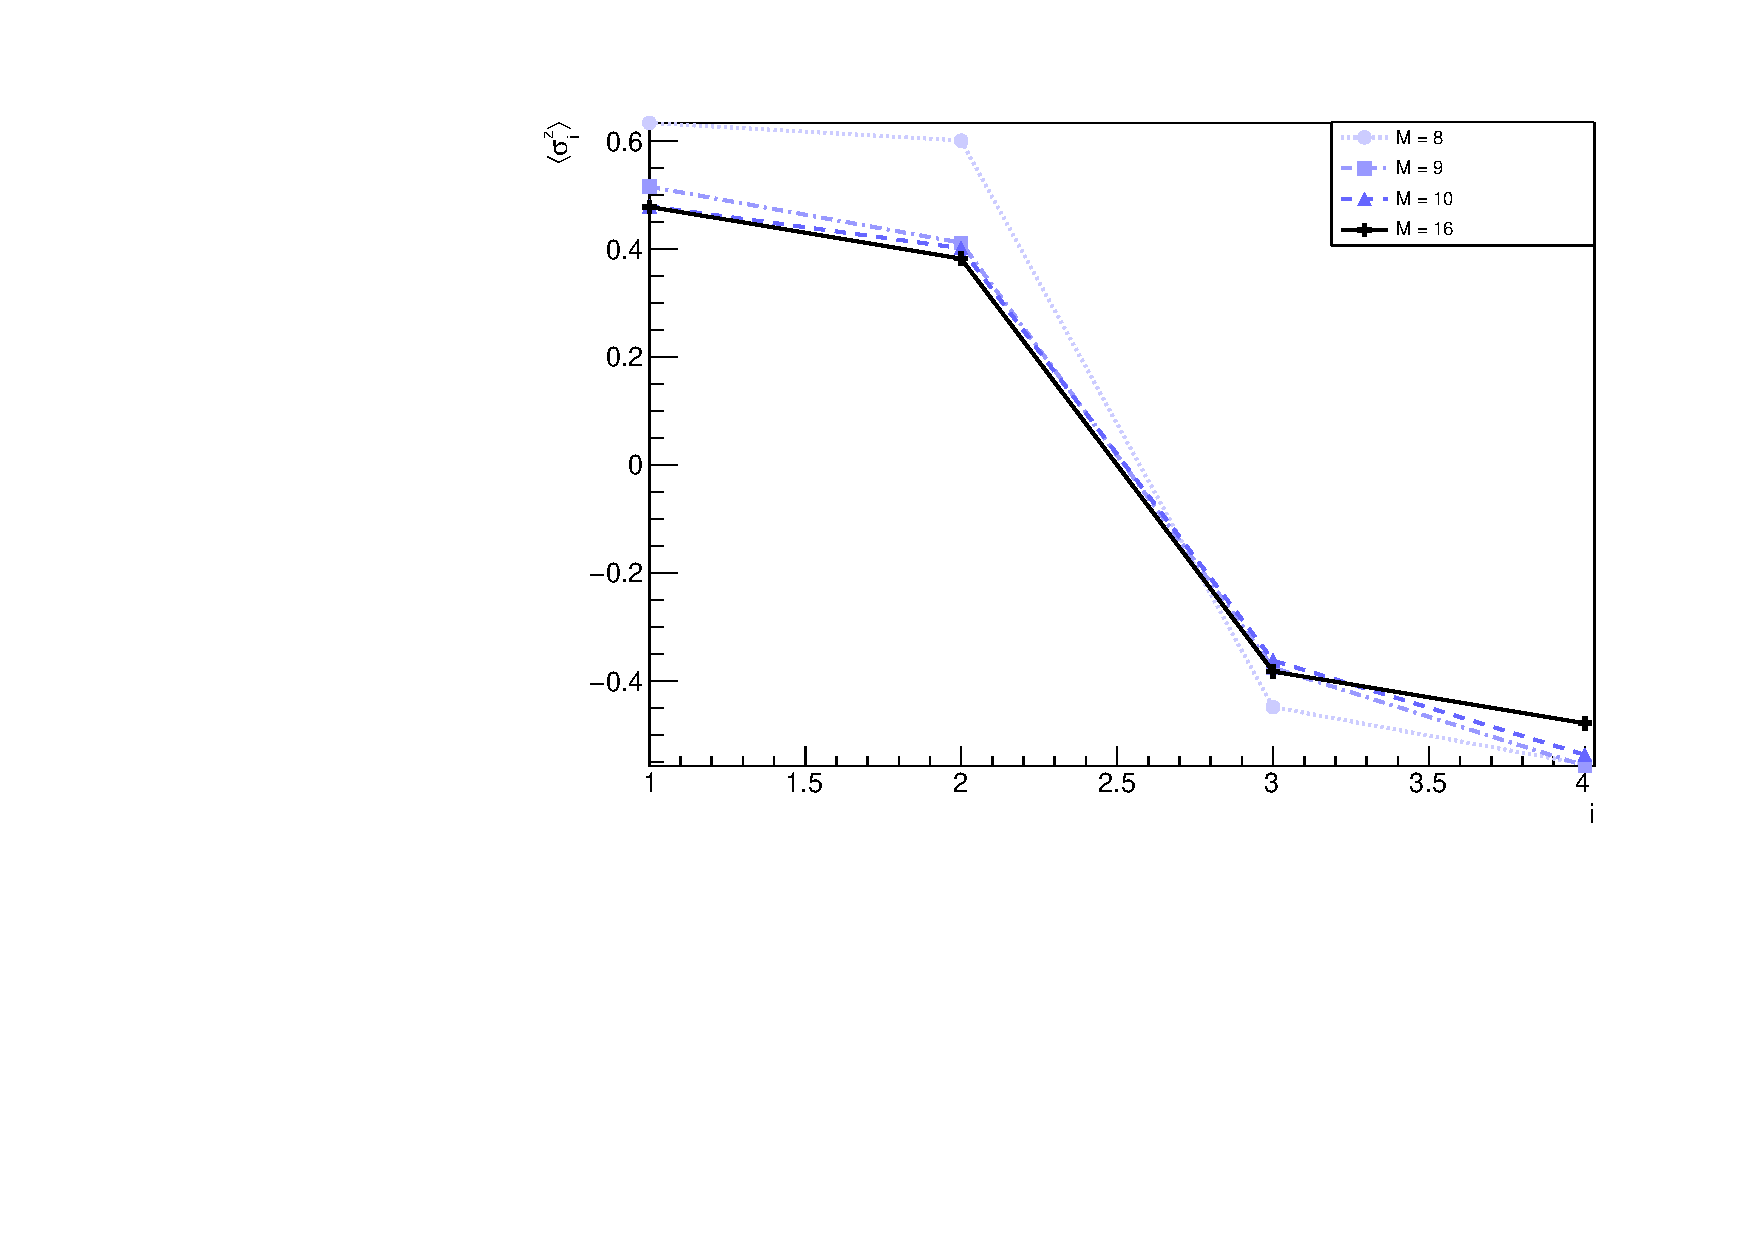
\includegraphics[scale=0.7]{Figures/4sites/4sites_totalDissipators.pdf}
    \caption{Caption}
    \label{fig:4sites_totalDissipators}
\end{figure}
%- 4-sites chain (model we want to study)
%- 4-sites chain (when it works)
%- 8 and 16-sites chain (when it doesn't work)
%- examples when it works





%%%%%%%%%%%%%%%%%%%%%%%%%%%%%%%%%%%%%%%%%%%%%%%%%%%%%%%%%%%%%%%%%%
%%%%%%%%%%%%%%%%%%%%%%%%%%%%%%%%%%%%%%%%%%%%%%%%%%%%%%%%%%%%%%%%%%
%%%%%%%%%%%%%%%%%%%%%%%%%%%%%%%%%%%%%%%%%%%%%%%%%%%%%%%%%%%%%%%%%%
\section{Convergence and Errors}

\begin{figure}[H]
    \label{fig:convergence_mpo_8sites}
    \centering
    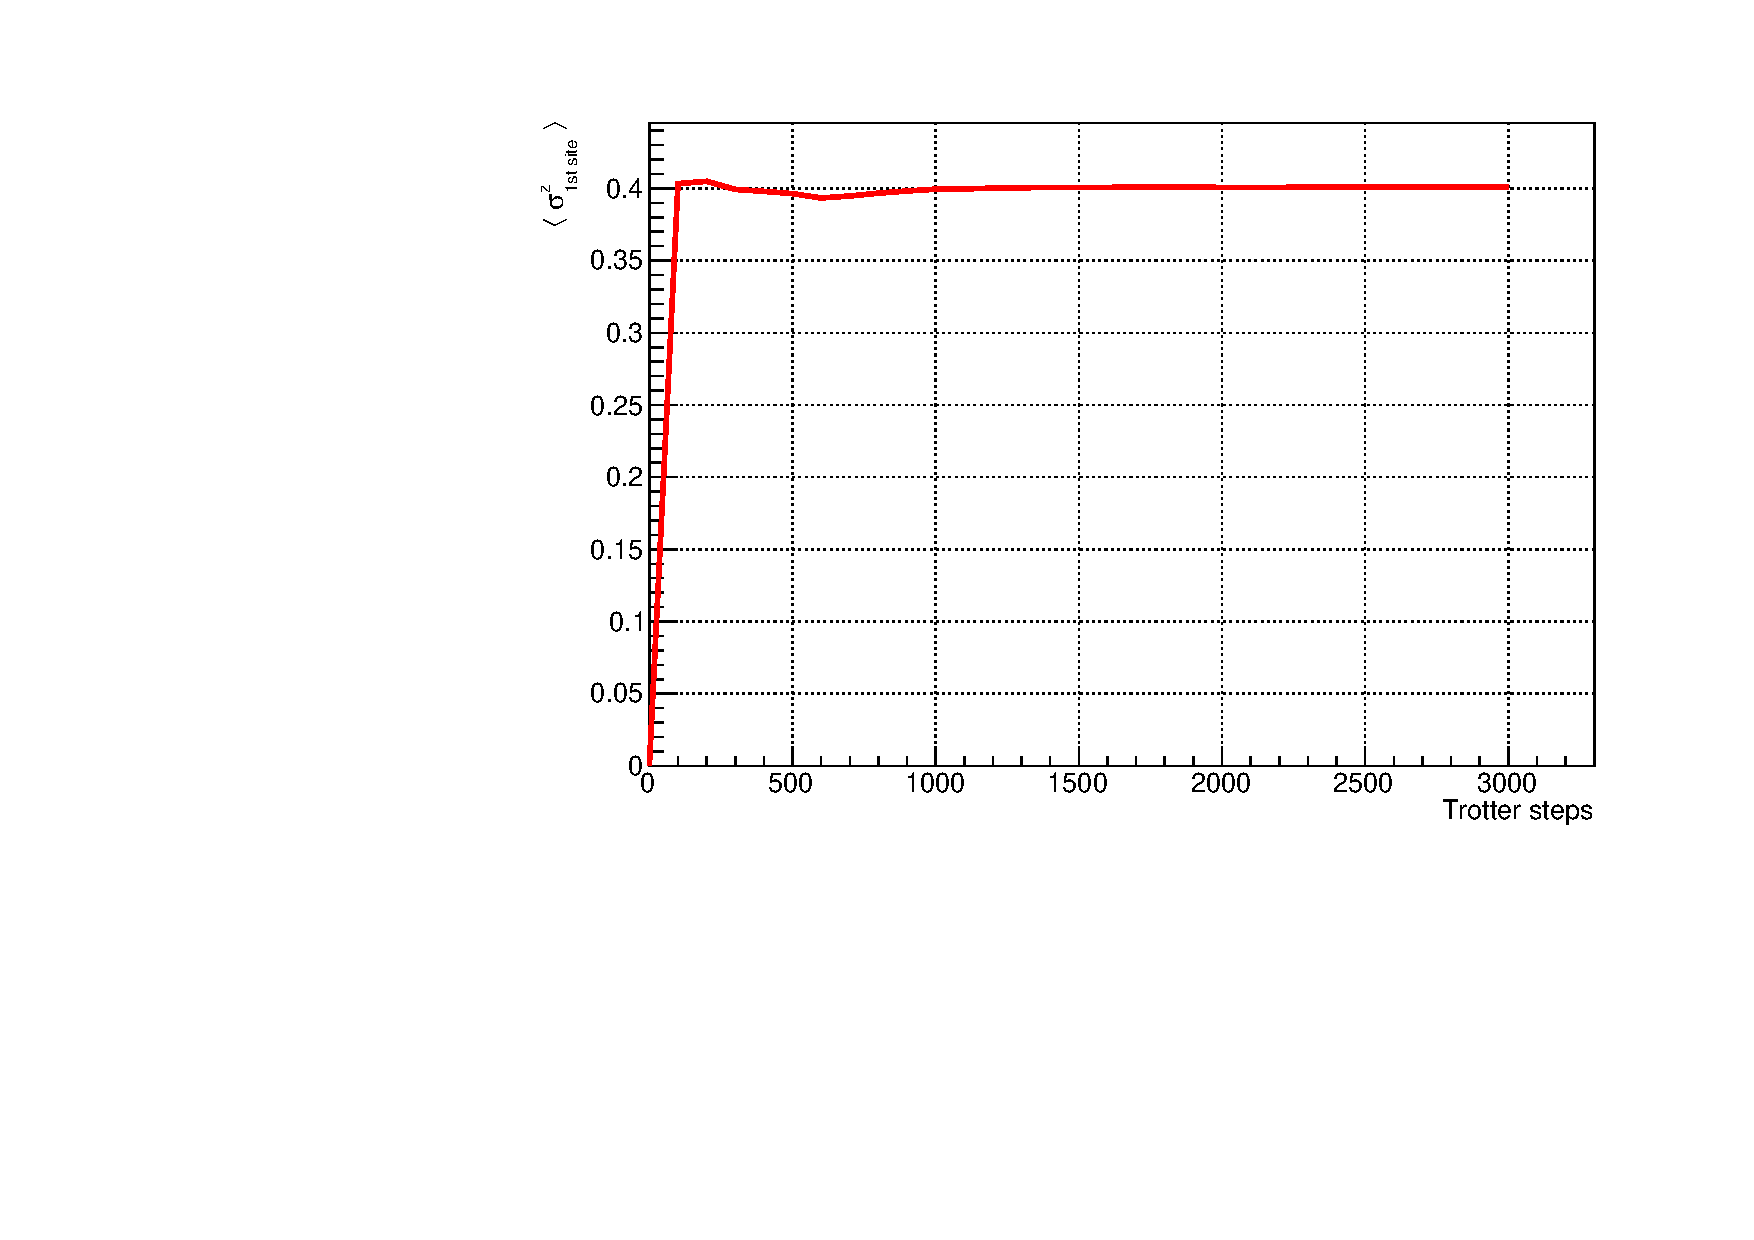
\includegraphics[scale=0.7]{Figures/convergence/Convergence_s8T3000J1051.pdf}
    \caption{Study of convergence of the MPO method for a 8-sites chain, for bond dimension m = 100 and T = 3000.}
    \label{fig:convergenceMPO_8sites}
\end{figure}

\begin{figure}[H]
    \label{fig:convergence_mpo_8sites}
    \centering
    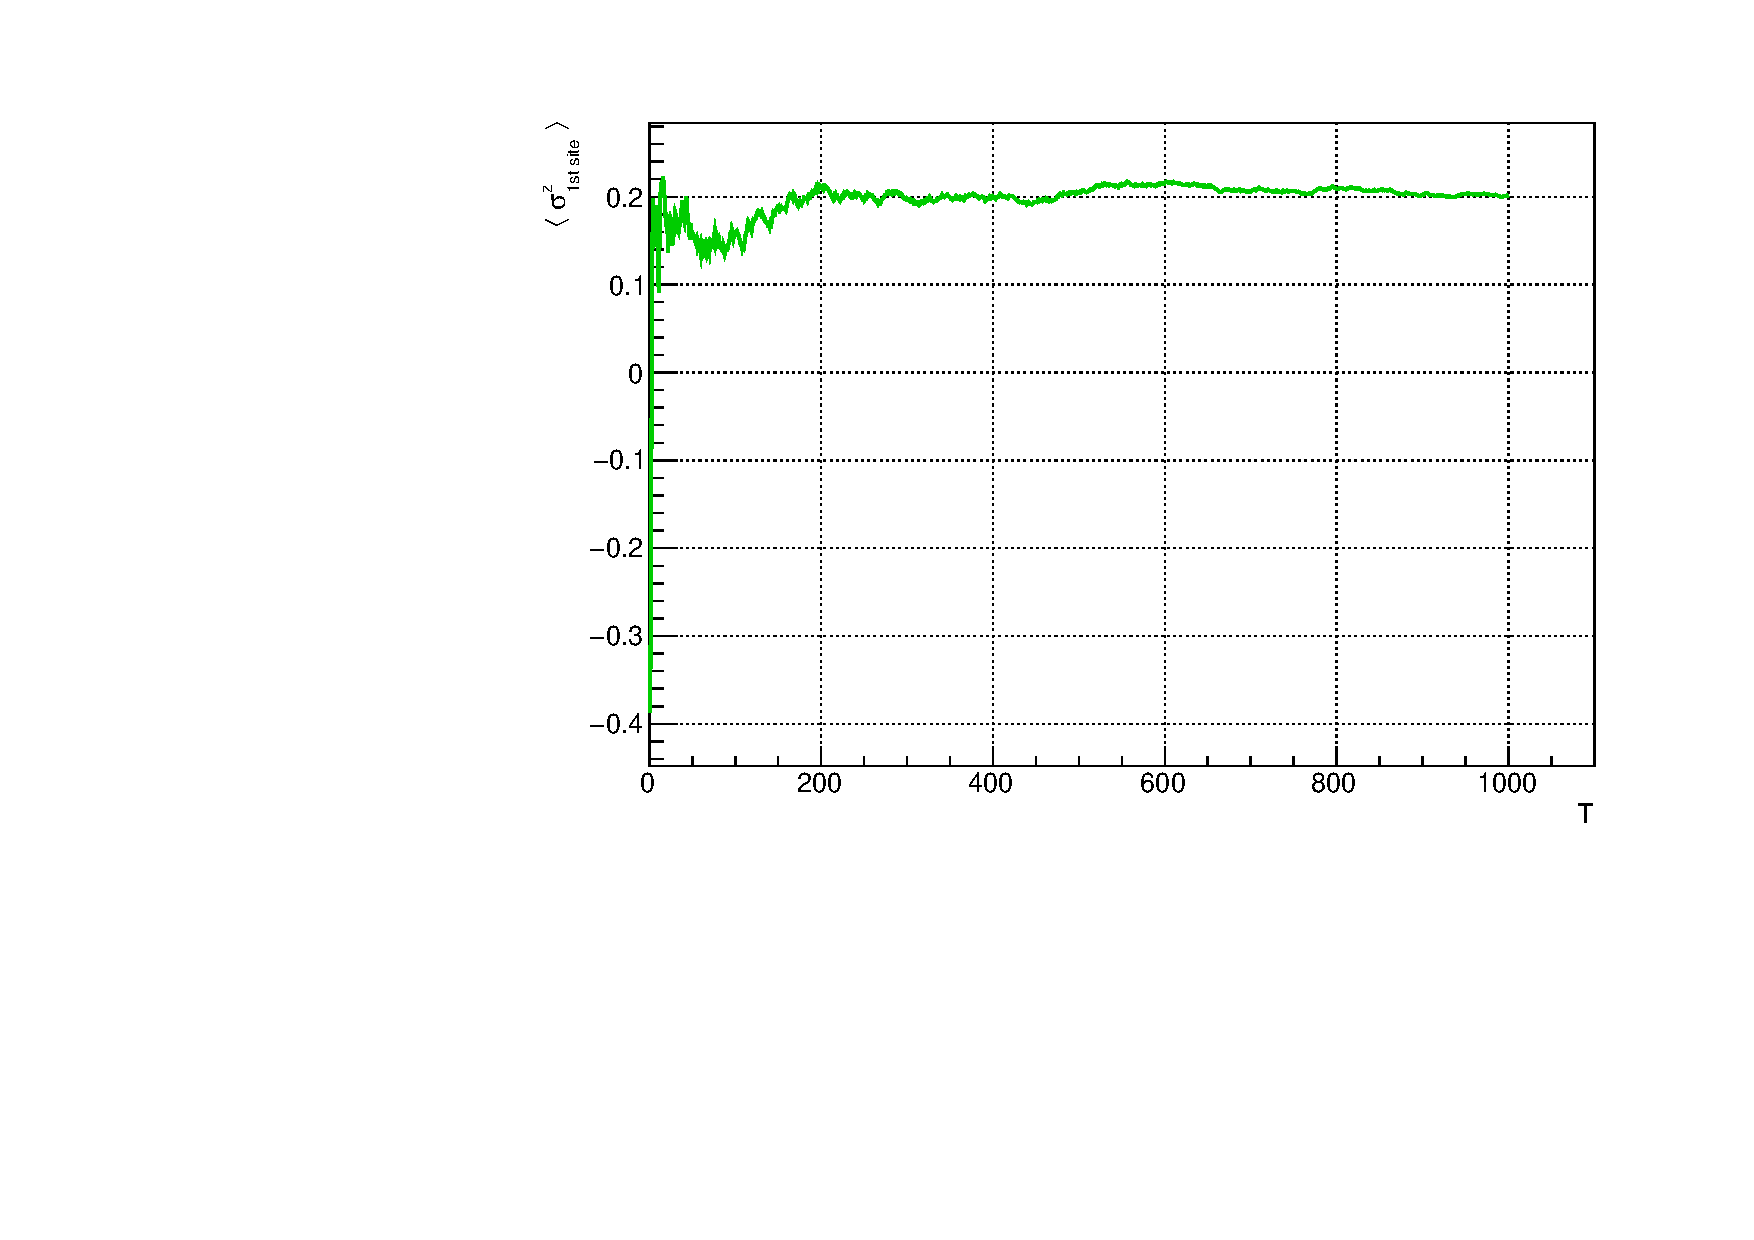
\includegraphics[scale=0.7]{Figures/convergence/Convergence_s8J10505.pdf}
    \caption{Study of convergence of the QT method for a 8-sites chain, for time step $dt=0.1$, T being the whole elapsed time.}
    \label{fig:convergenceMPO_8sites}
\end{figure}

\begin{figure}[H]
    \centering
    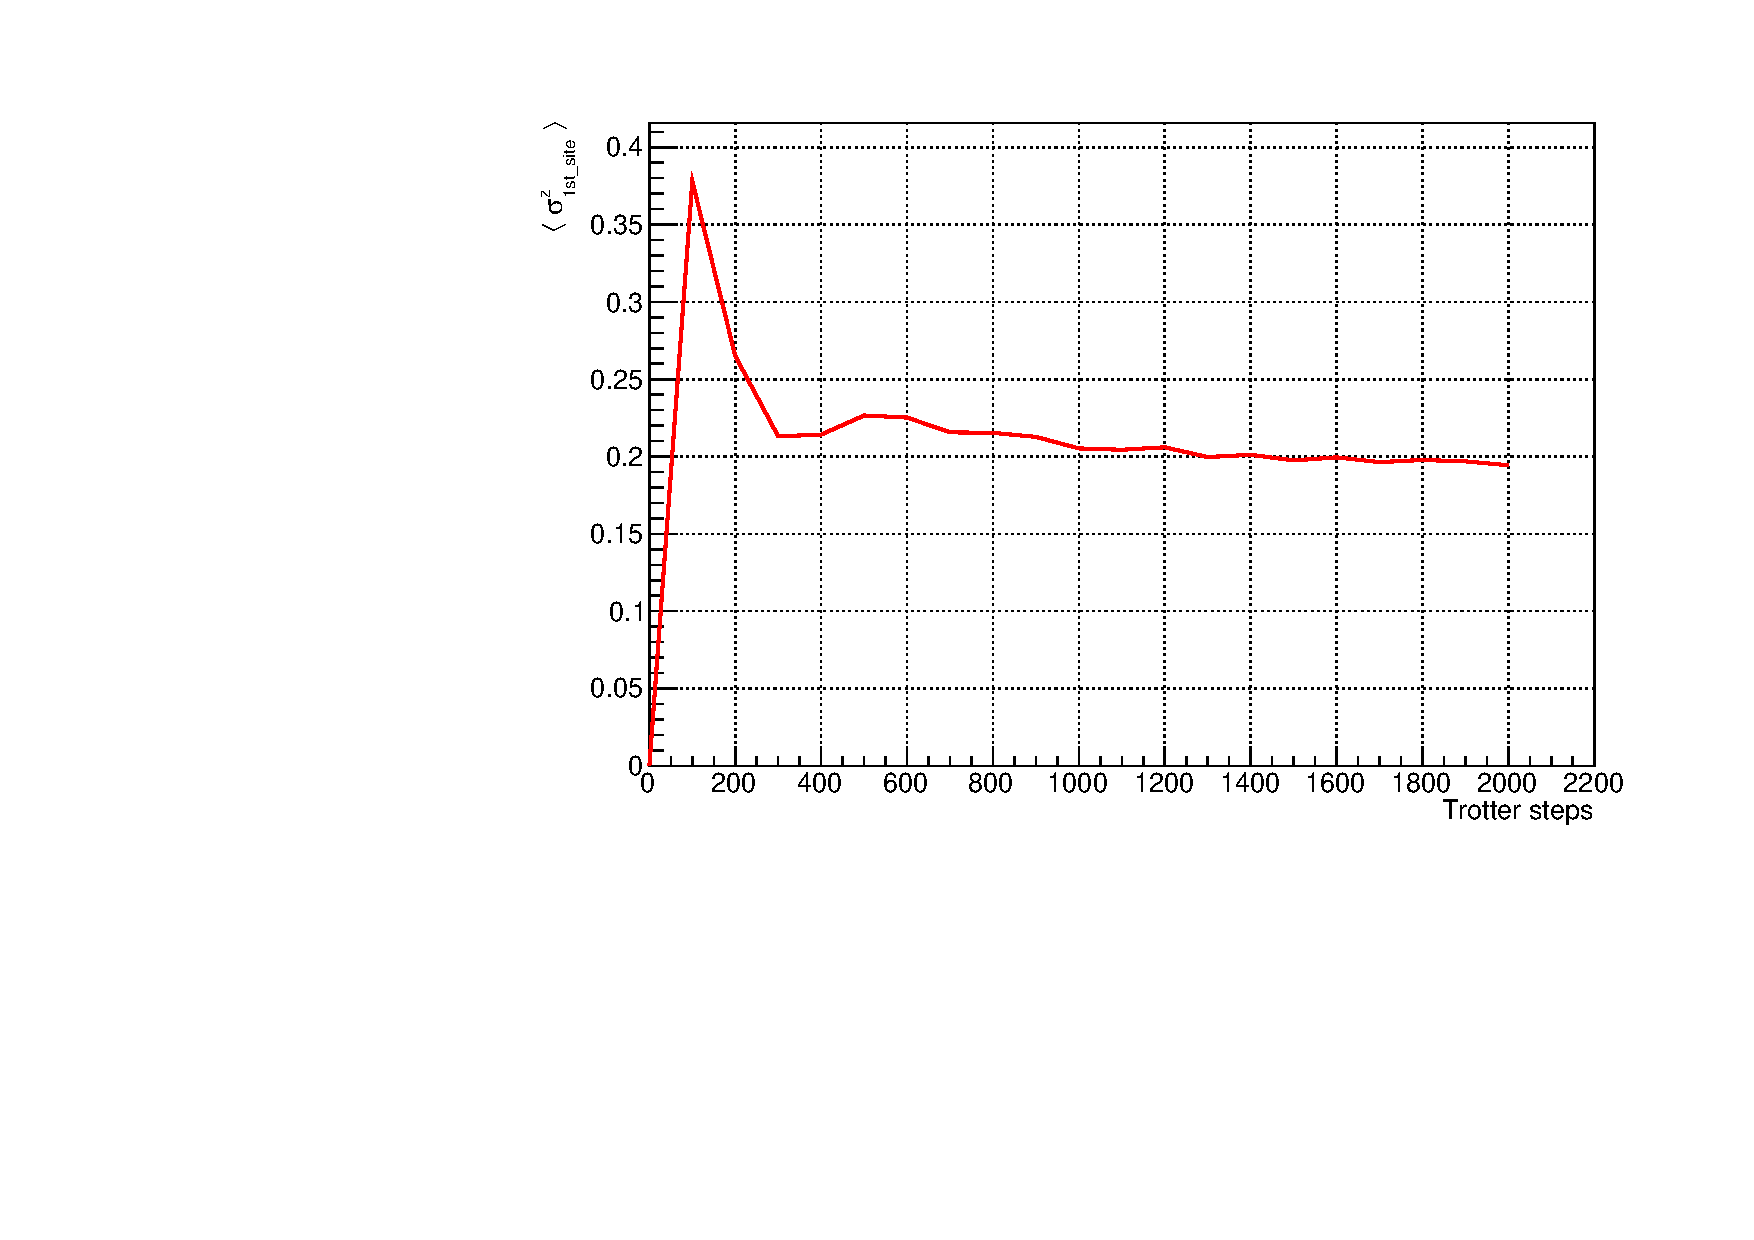
\includegraphics[scale=0.7]{Figures/12sites/ConvergenceLML012m060Time002000_J10505.pdf}
    \caption{Study of convergence of the MPO method for a 12-sites chain, for bond dimension m = 60 and T = 2000.}
    \label{fig:my_label}
\end{figure}

\textcolor{red}{NUMERICAL ERRORS?}

%%%%%%%%%%%%%%%%%%%%%%%%%%%%%%%%%%%%%%%%%%%%%%%%%%%%%%%%%%%%%%%%%%
%%%%%%%%%%%%%%%%%%%%%%%%%%%%%%%%%%%%%%%%%%%%%%%%%%%%%%%%%%%%%%%%%%
%%%%%%%%%%%%%%%%%%%%%%%%%%%%%%%%%%%%%%%%%%%%%%%%%%%%%%%%%%%%%%%%%%
\section{Magnetization Profile}
The first observable we are going to examine is the magnetization profile of the chain, i.e. the expectation value $\langle \sigma^z \rangle$ of the Pauli spin- matrix $\sigma^z$ for each site. 

\begin{figure}[H]
    \centering
    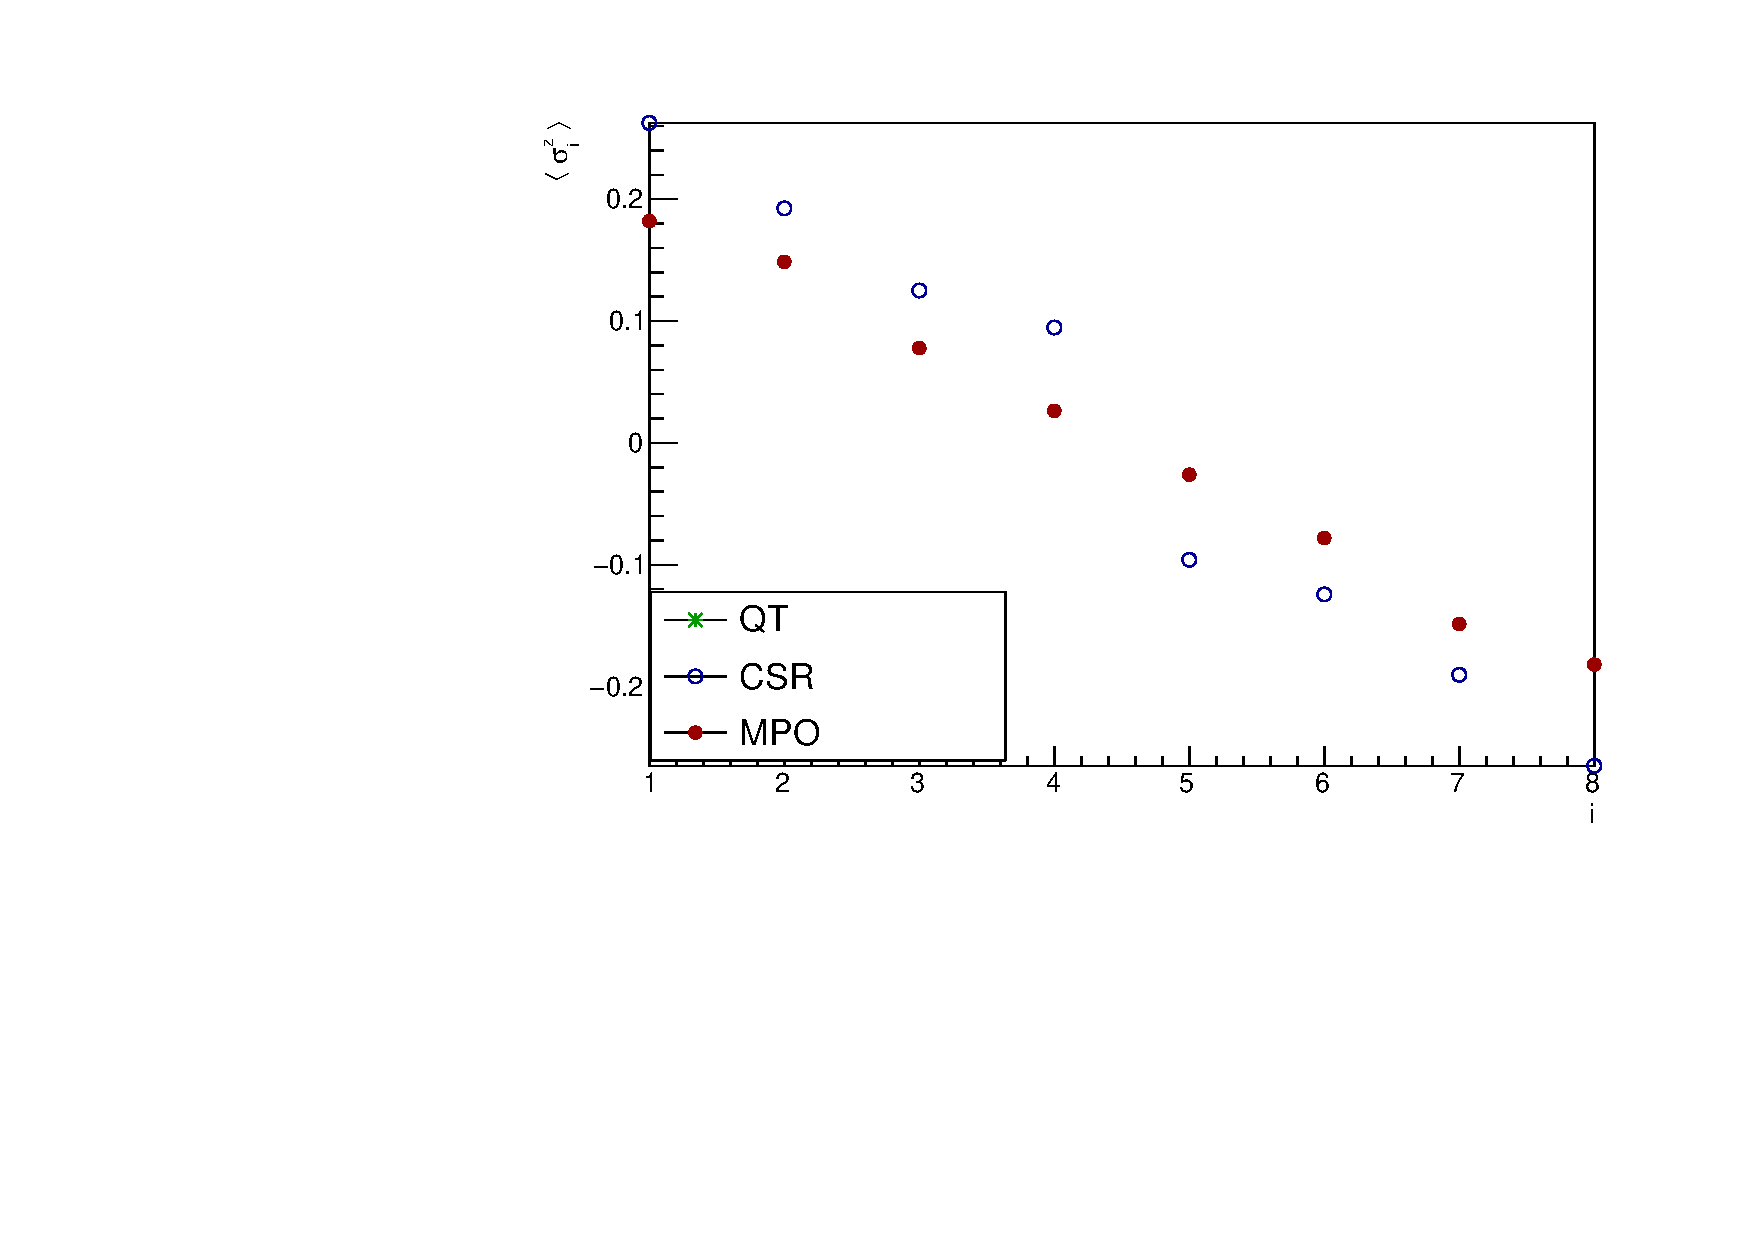
\includegraphics[scale=0.7]{Figures/8sites_comparison/LMComparison_8sJ10505.pdf}
    \caption{Spin profile for a 8-sites chain characterized by $\gamma~=~1, J_x=1, J_y=0.5, J_z=0.5$; \emph{i} stands for the site index.}
    \label{fig:8sites_LMcomparisonJz05}
\end{figure}

\begin{figure}[H]
    \centering
    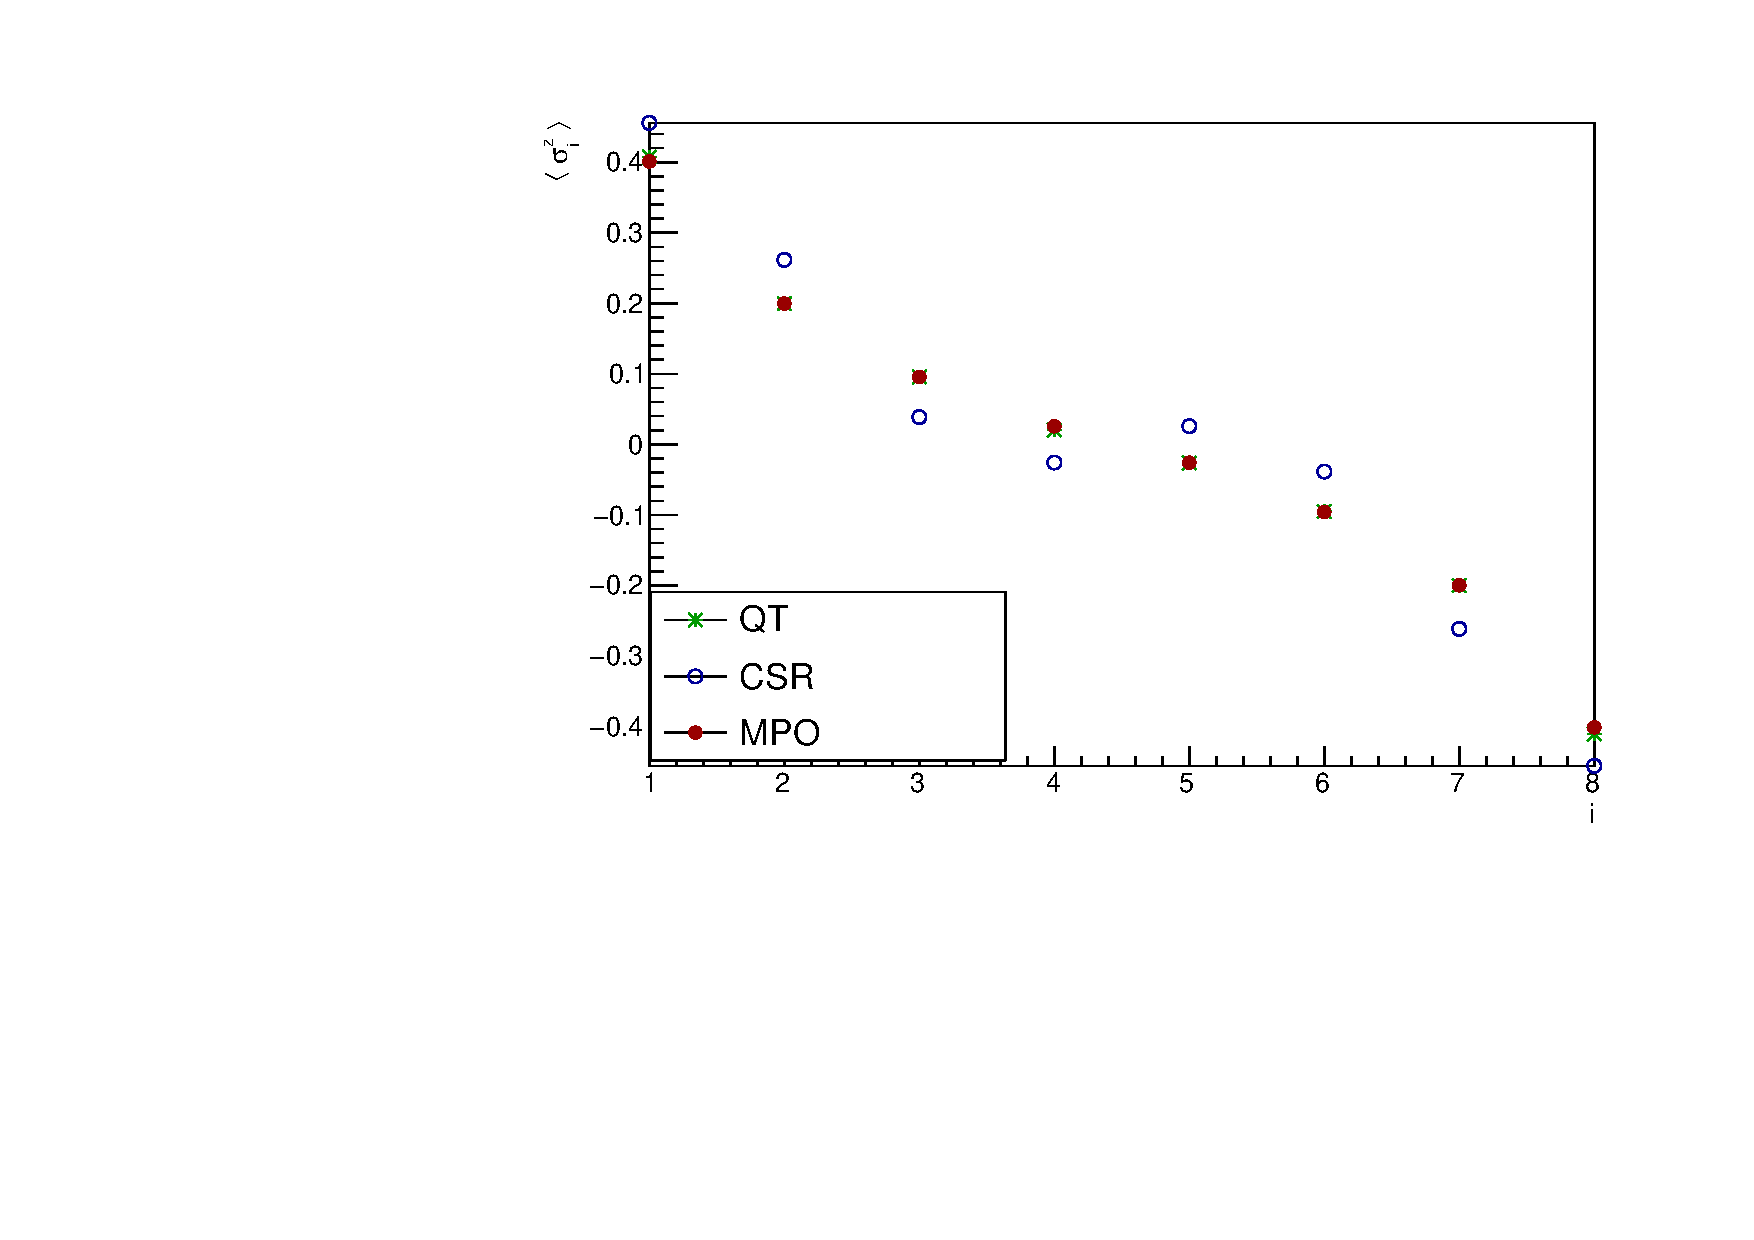
\includegraphics[scale=0.7]{Figures/8sites_comparison/LMComparison_8sJ1051.pdf}
    \caption{Spin profile for a 8-sites chain characterized by $\gamma~=~1, J_x=1, J_y=0.5, J_z=1$; \emph{i} stands for the site index.}
    \label{fig:8sites_LMcomparisonJz1}
\end{figure}

\begin{figure}[H]
    \centering
    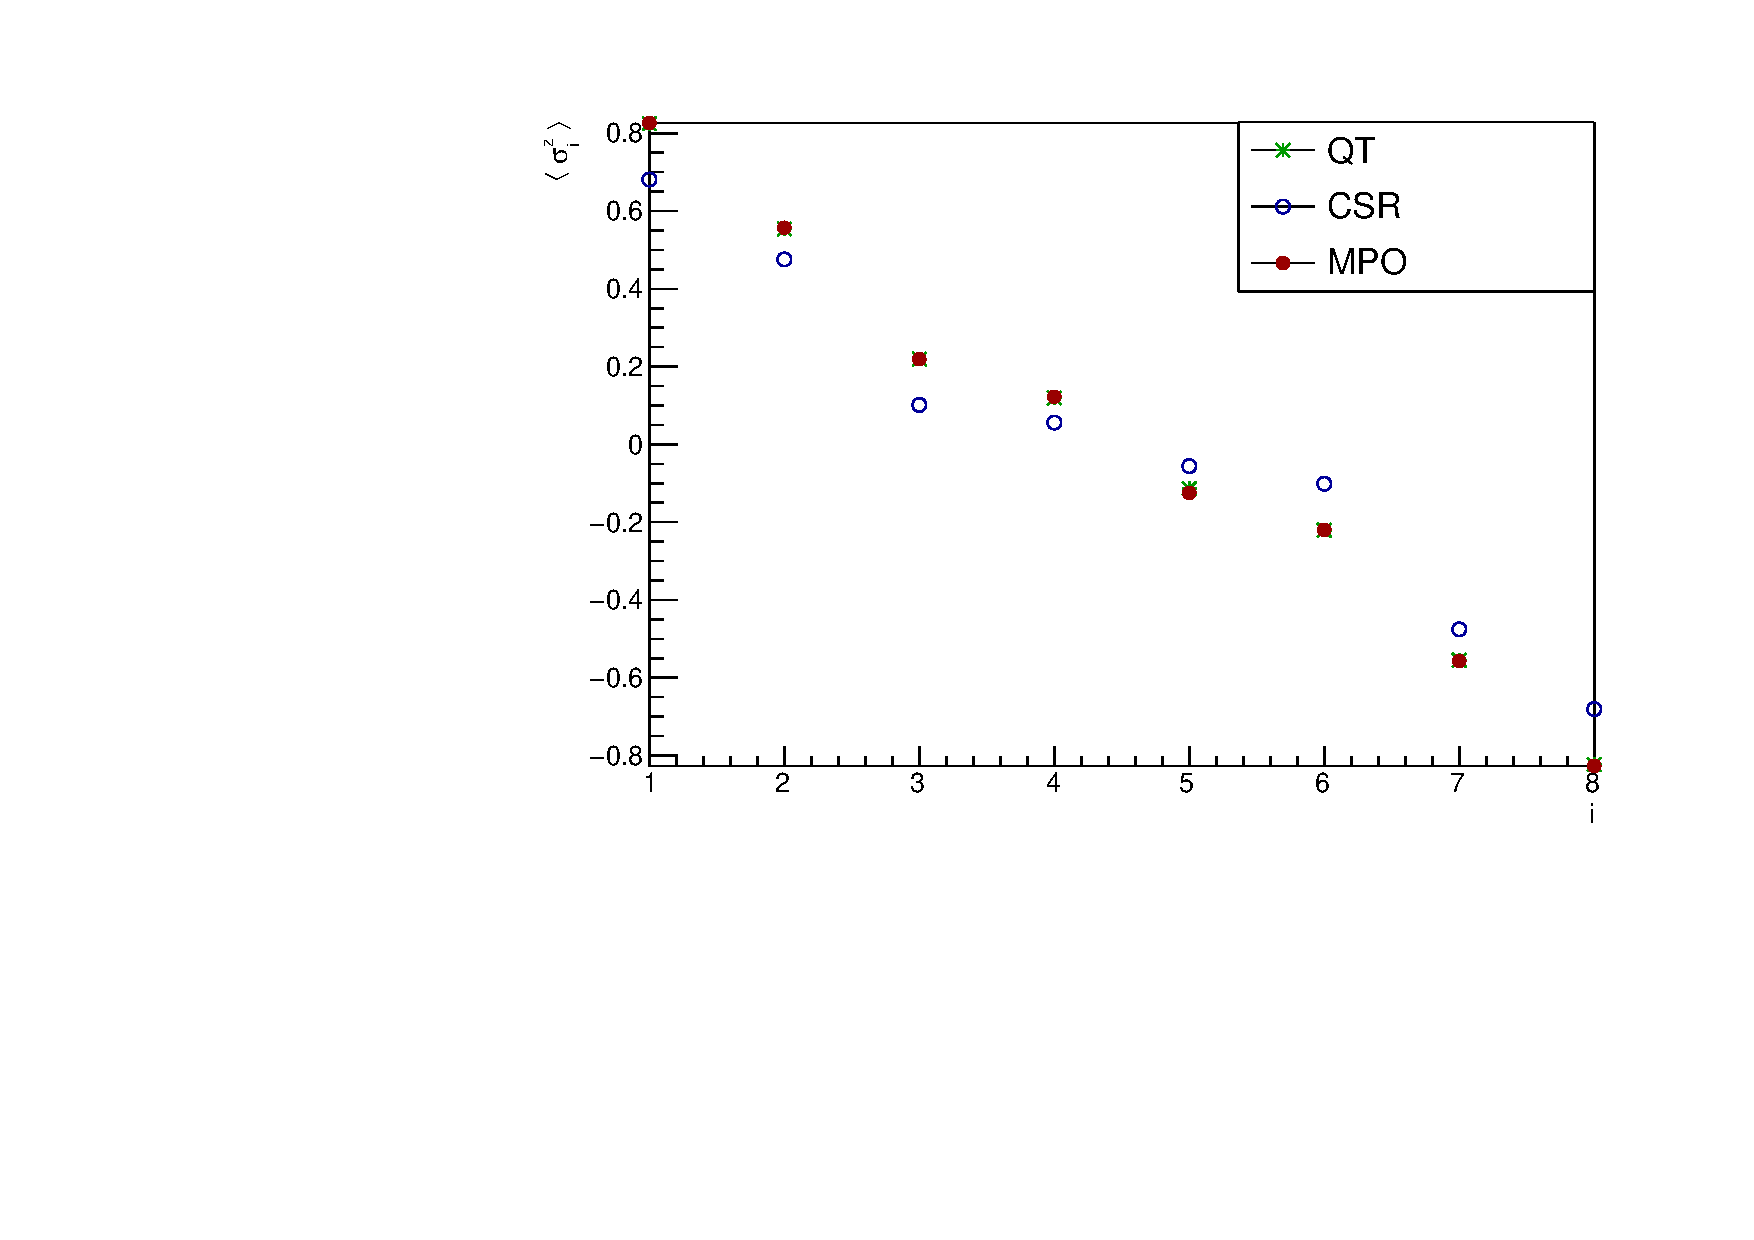
\includegraphics[scale=0.7]{Figures/8sites_comparison/LM_8s_J10515.pdf}
    \caption{Spin profile for a 8-sites chain characterized by $\gamma~=~1, J_x=1, J_y=0.5, J_z=1.5$.}
    \label{fig:my_label}
\end{figure}

It can be interesting seeing if the magnetization changes its profile for different chain lengths; now let us see the case of a \textbf{12-sites} chain for different values of $J_z$ as done previously. The following data are obtained from MPO method.

\begin{figure}[H]
    \centering
    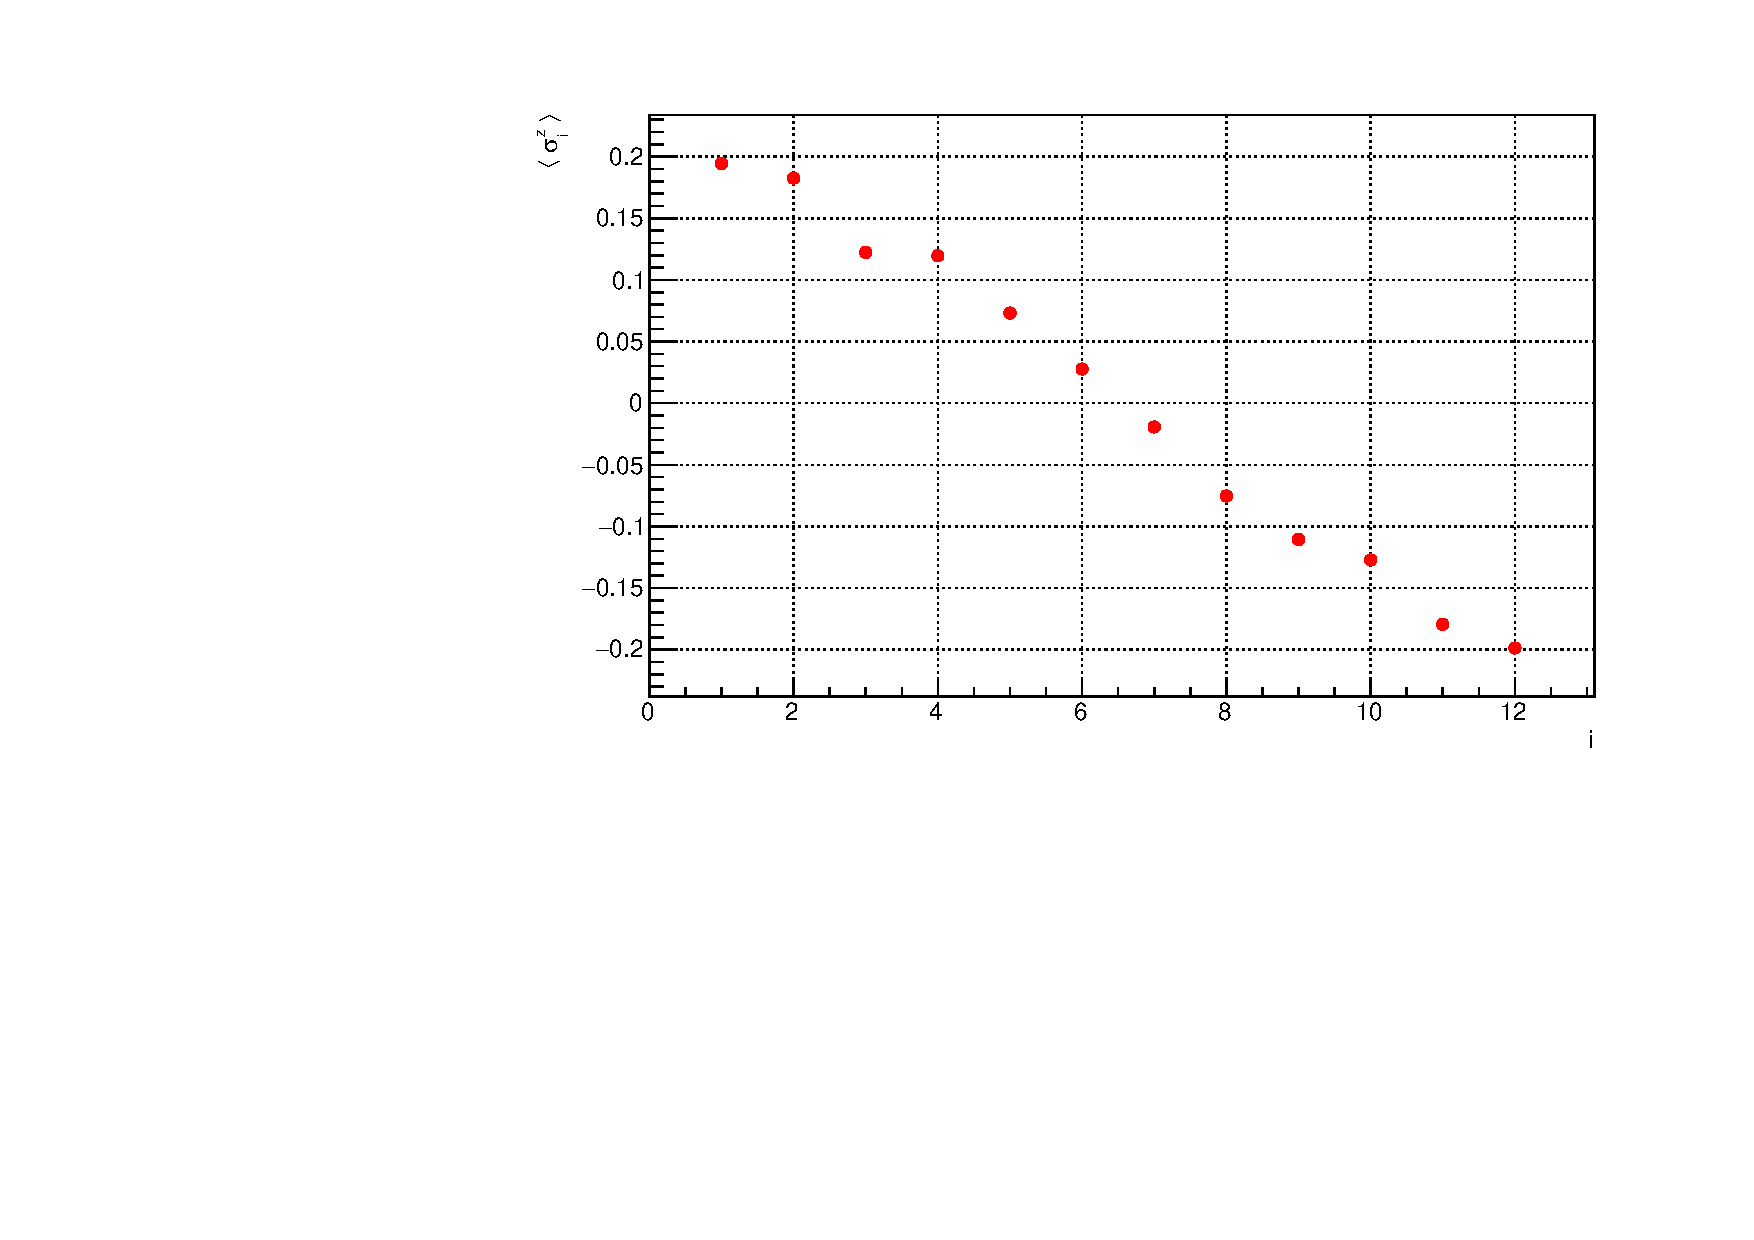
\includegraphics[scale=0.7]{Figures/12sites/LML012m060Time002000_J10505.pdf}
    \caption{Spin profile for a 12-sites chain characterized by $\gamma~=~1, J_x=1, J_y=0.5, J_z=0.5$. Data are obtained from MPO method, with m = 60 and T = 2000.}
    \label{fig:my_label}
\end{figure}

\begin{figure}[H]
    \centering
    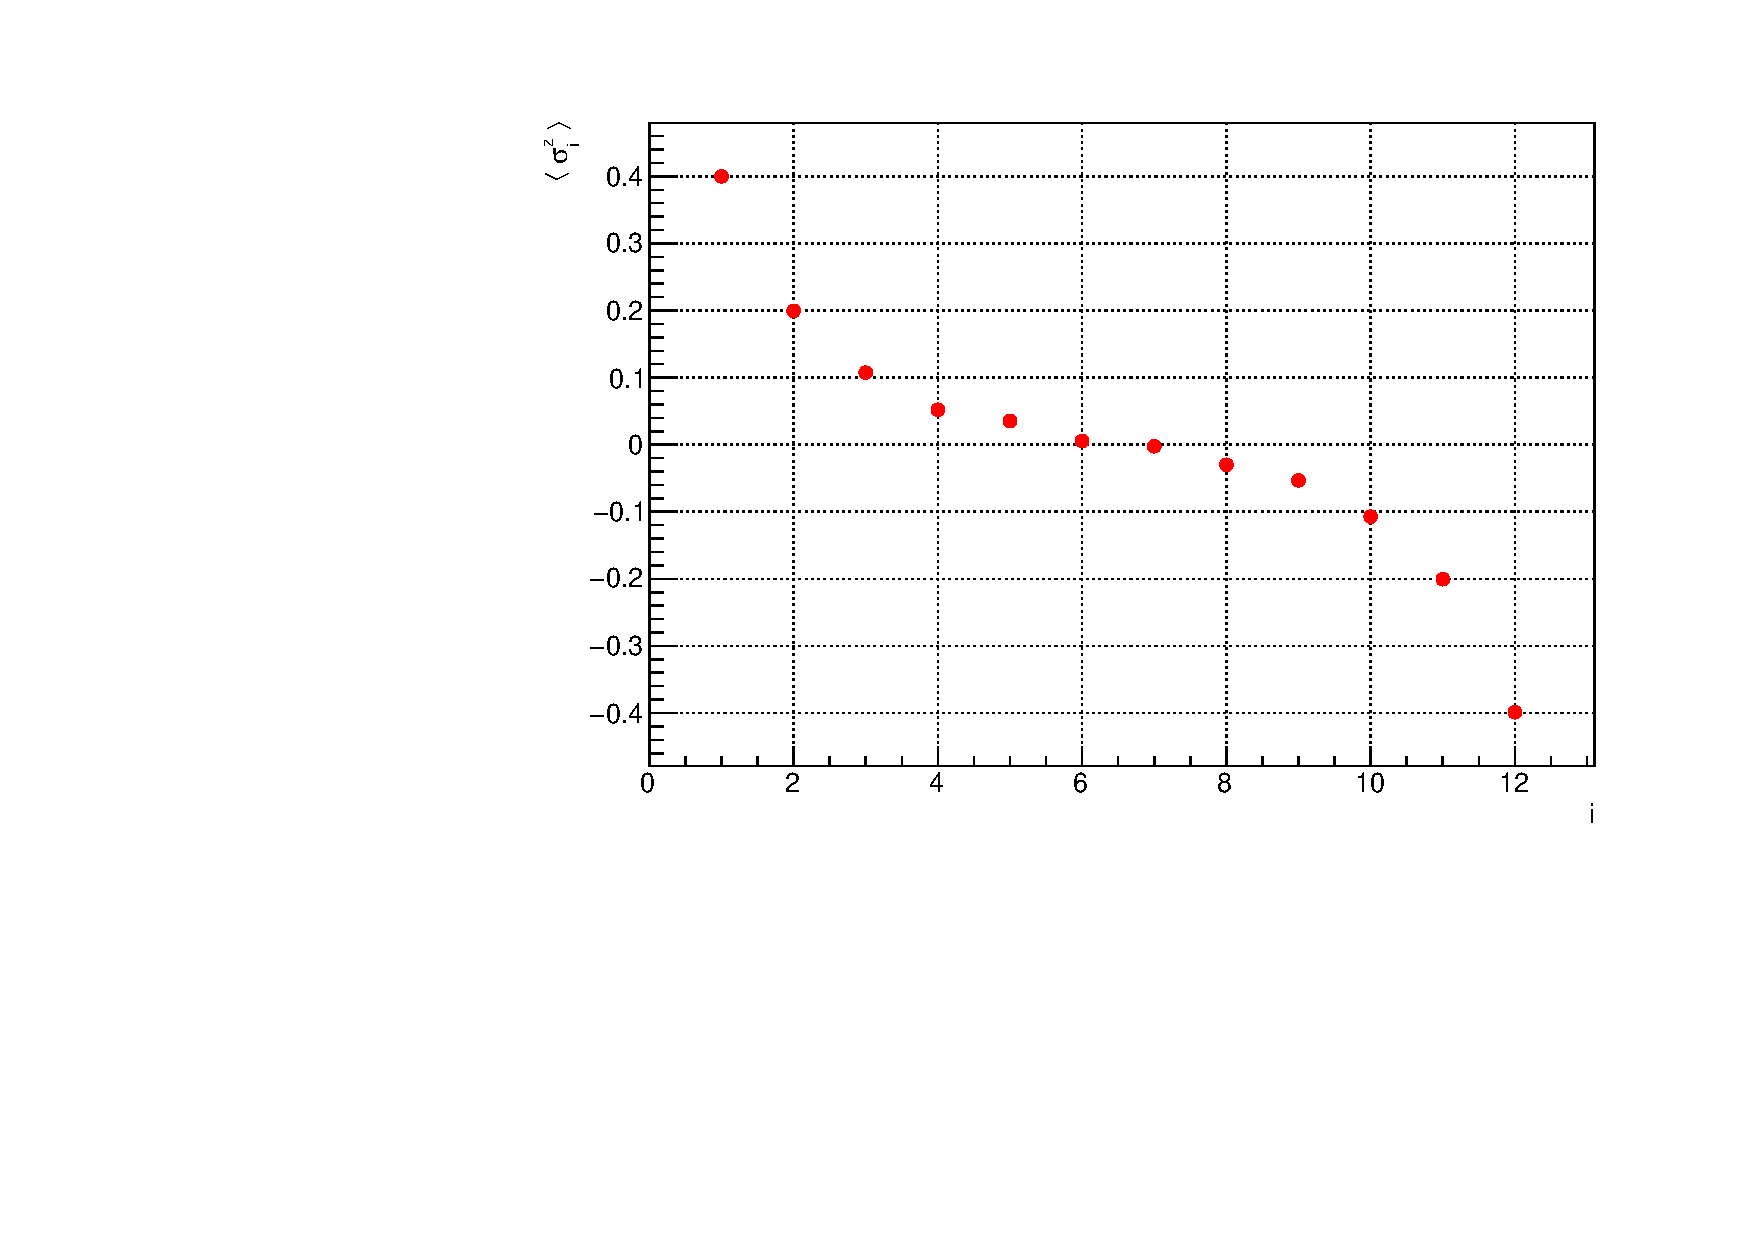
\includegraphics[scale=0.7]{Figures/12sites/LML012m060Time002000_J1051.pdf}
    \caption{Spin profile for a 12-sites chain characterized by $\gamma~=~1, J_x=1, J_y=0.5, J_z=1.$. Data are obtained from MPO method, with m = 60 and T = 2000.}
    \label{fig:my_label}
\end{figure}

\begin{figure}[H]
    \centering
    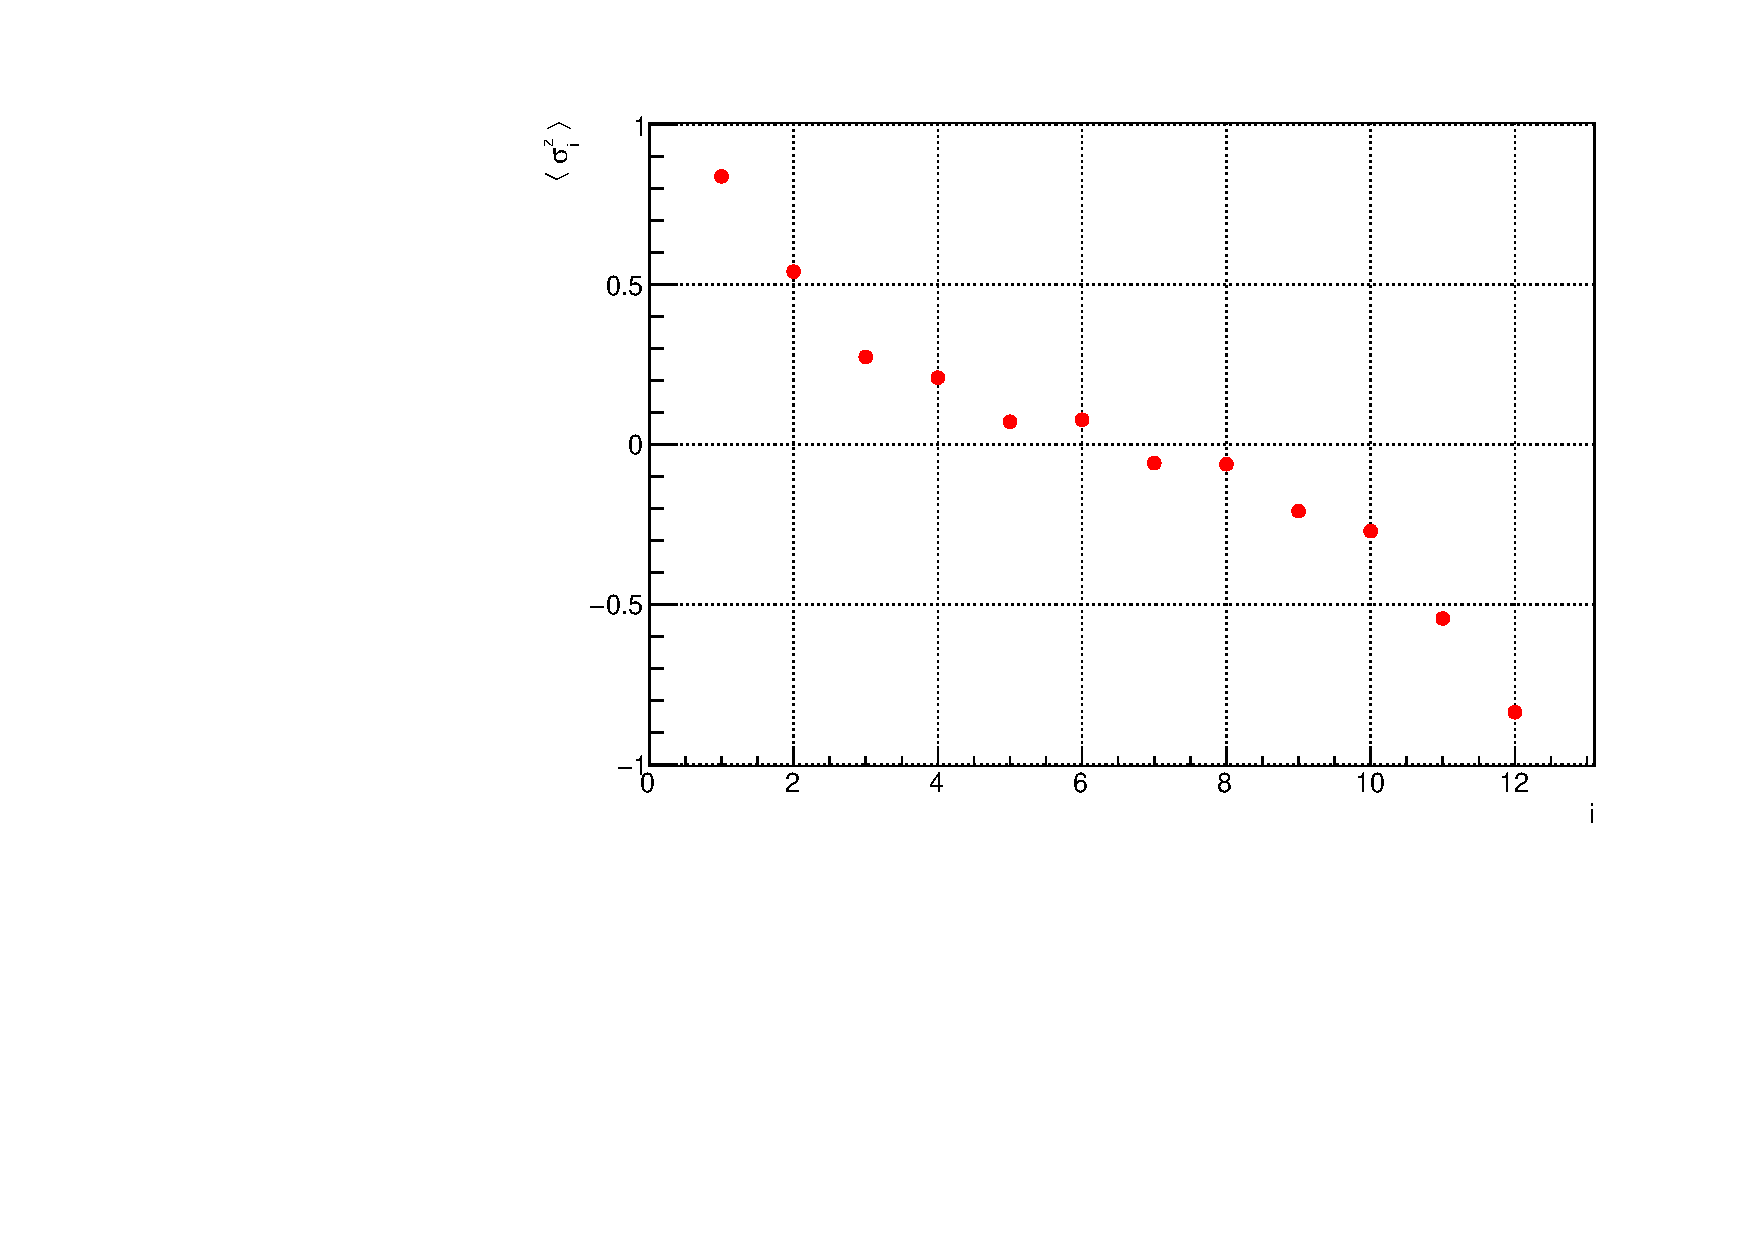
\includegraphics[scale=0.7]{Figures/12sites/LML012m060Time002000_J10515.pdf}
    \caption{Spin profile for a 12-sites chain characterized by $\gamma~=~1, J_x=1, J_y=0.5, J_z=1.5$. Data are obtained from MPO method, with m = 60 and T = 2000.}
    \label{fig:my_label}
\end{figure}

Let us see \textbf{16-sites} chain.

\begin{figure}[H]
    \centering
    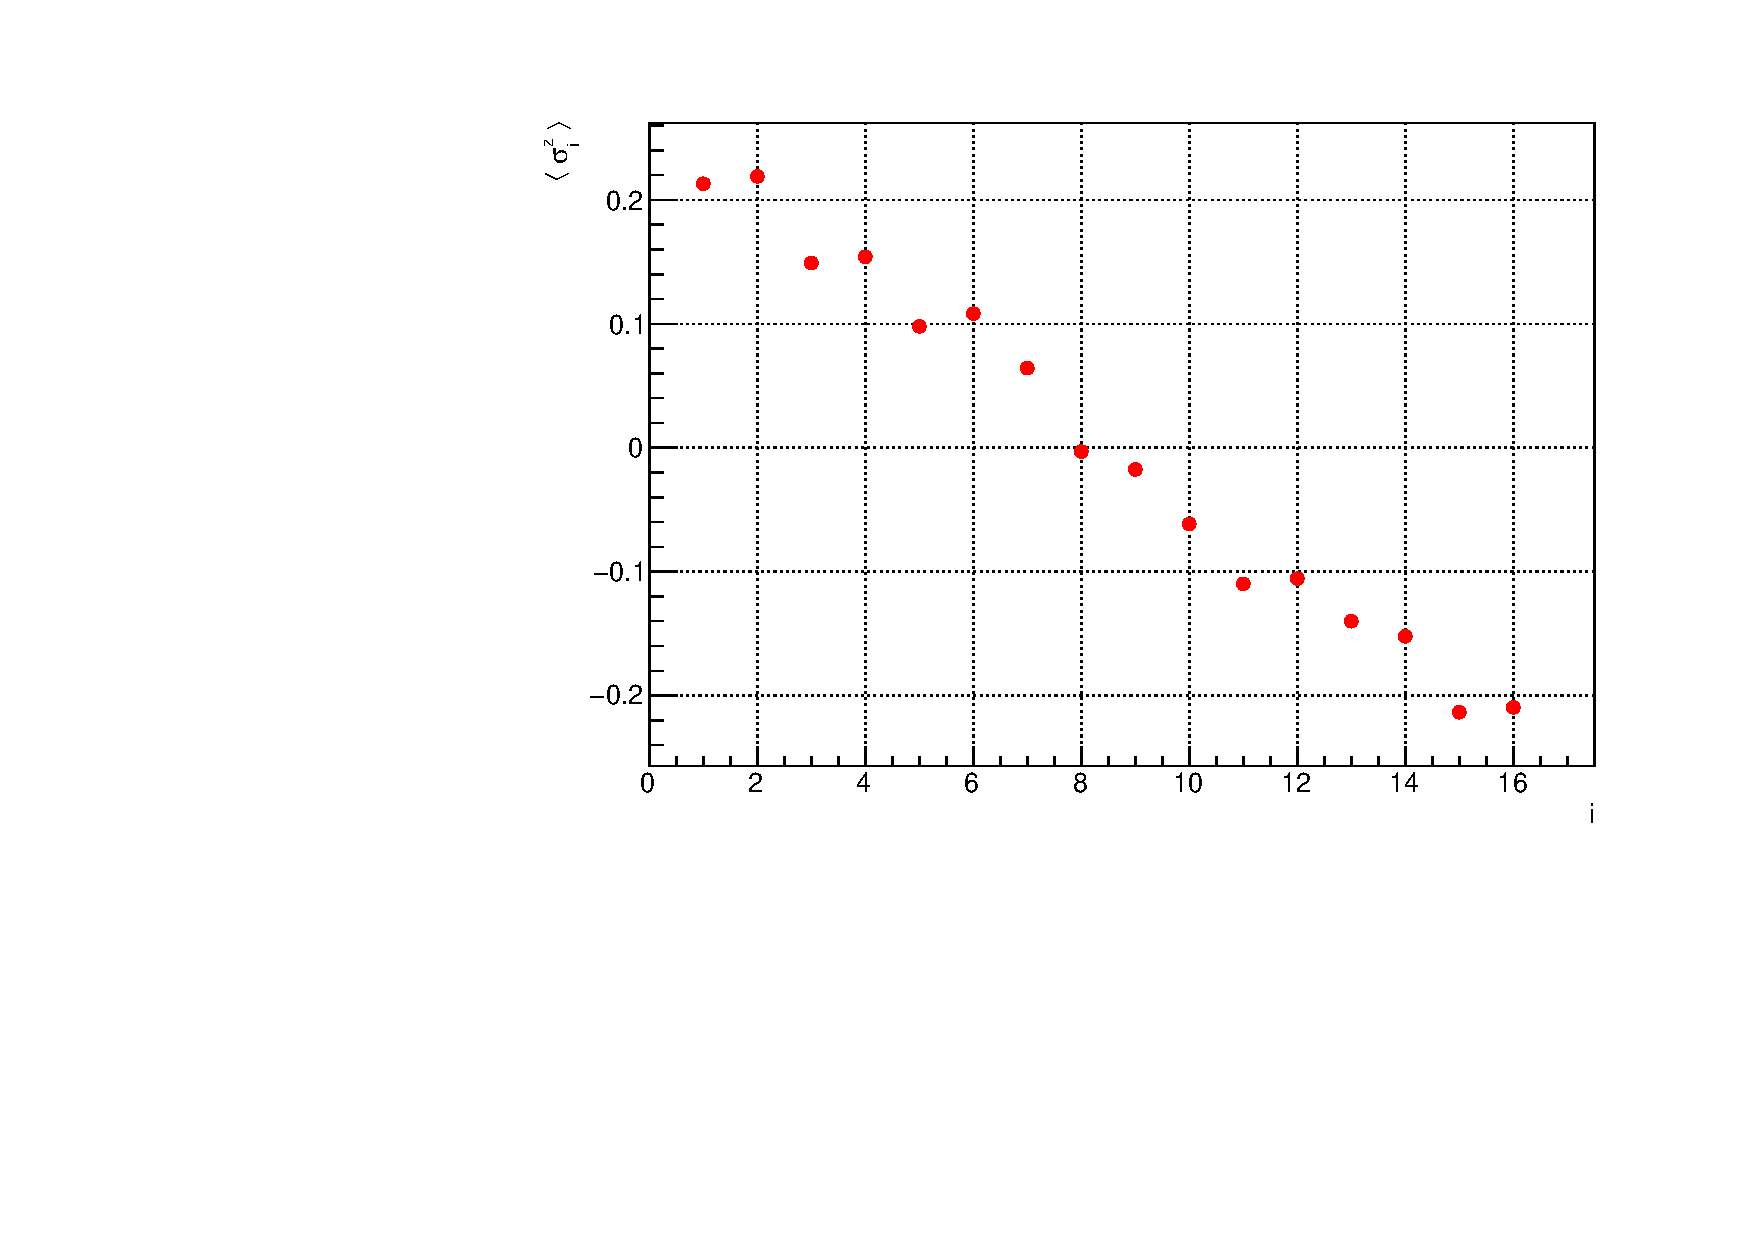
\includegraphics[scale=0.7]{Figures/16sites/LML016m080Time001000_J10505.pdf}
    \caption{Spin profile for a 16-sites chain characterized by $\gamma~=~1, J_x=1, J_y=0.5, J_z=0.5$. Data are obtained from MPO method, with m = 80 and T = 1000.}
    \label{fig:my_label}
\end{figure}

\begin{figure}[H]
    \centering
    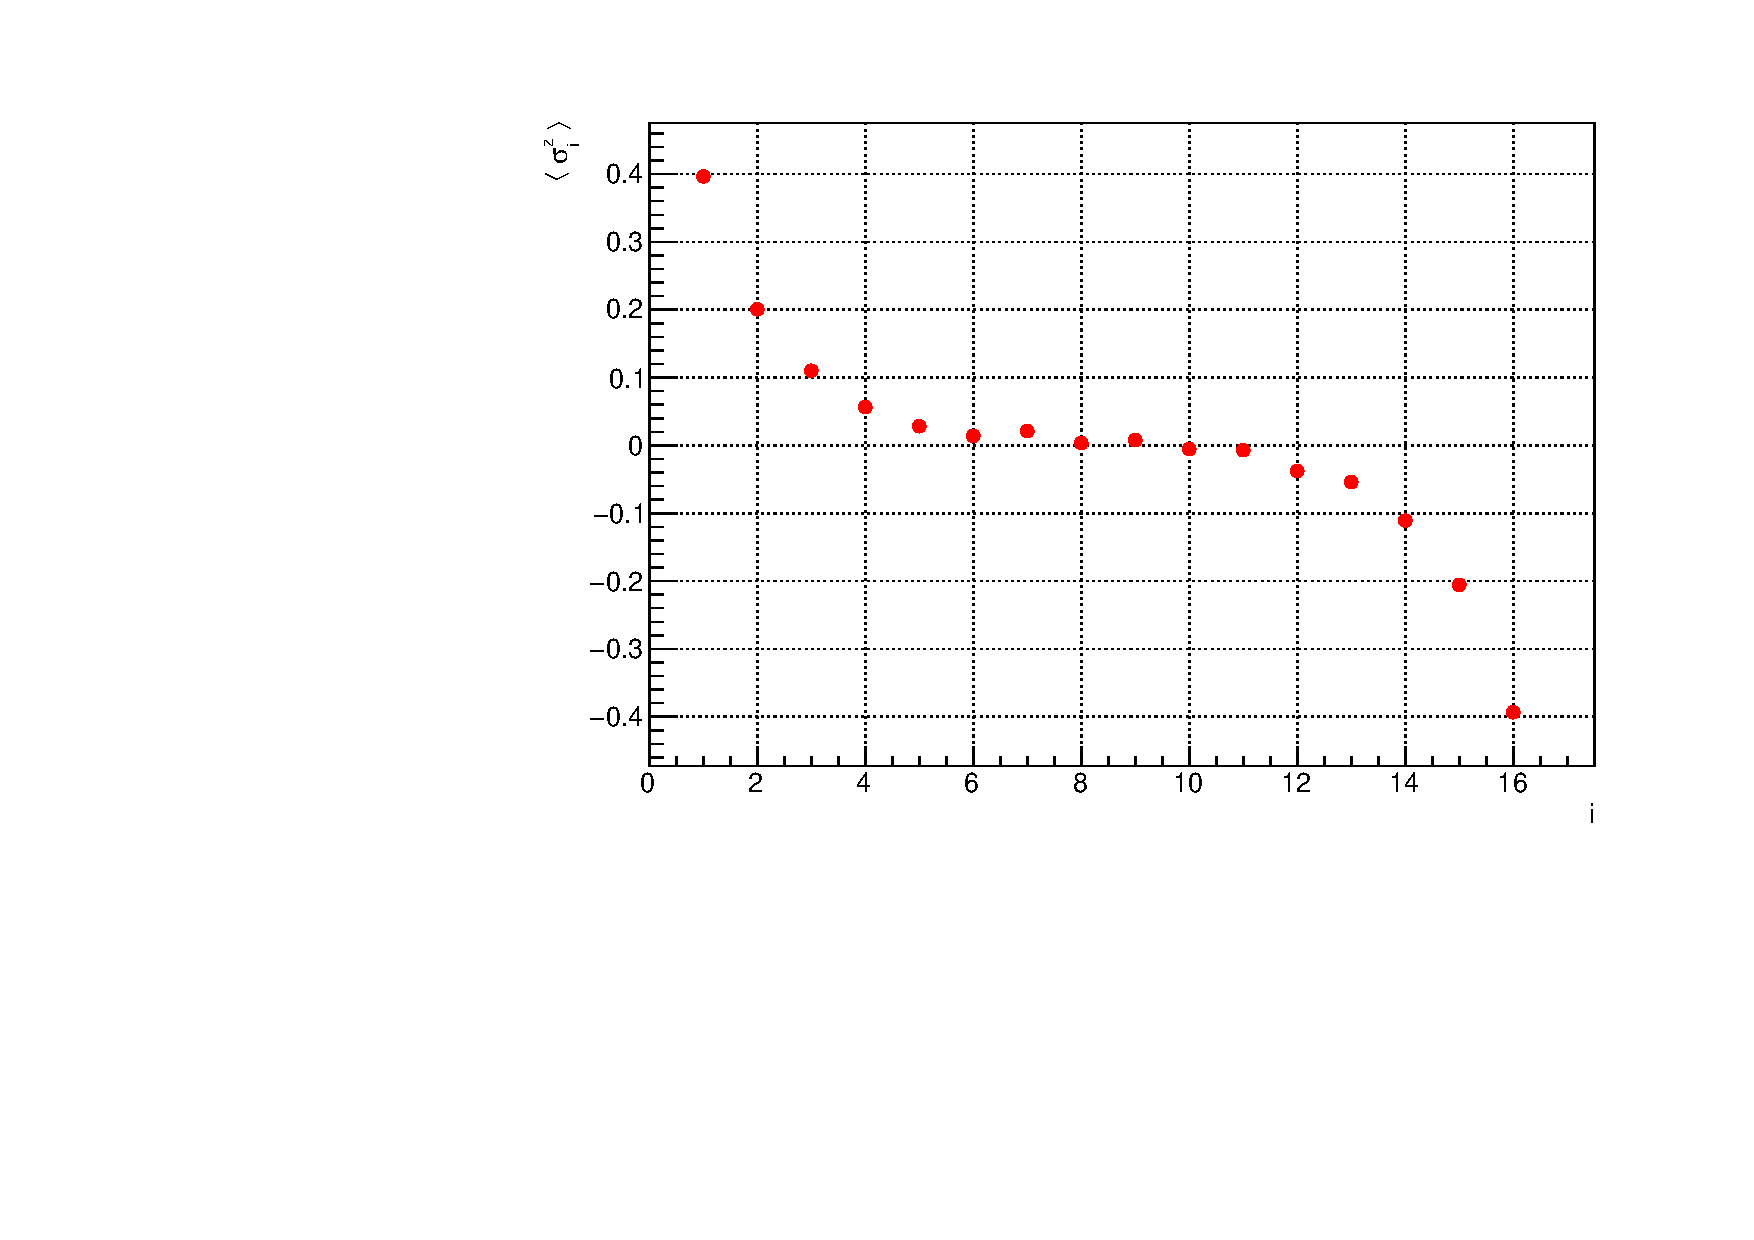
\includegraphics[scale=0.7]{Figures/16sites/LML016m080Time002500_J1051.pdf}
    \caption{Spin profile for a 16-sites chain characterized by $\gamma~=~1, J_x=1, J_y=0.5, J_z=1.$. Data are obtained from MPO method, with m = 80 and T = 2500.}
    \label{fig:my_label}
\end{figure}

\begin{figure}[H]
    \centering
    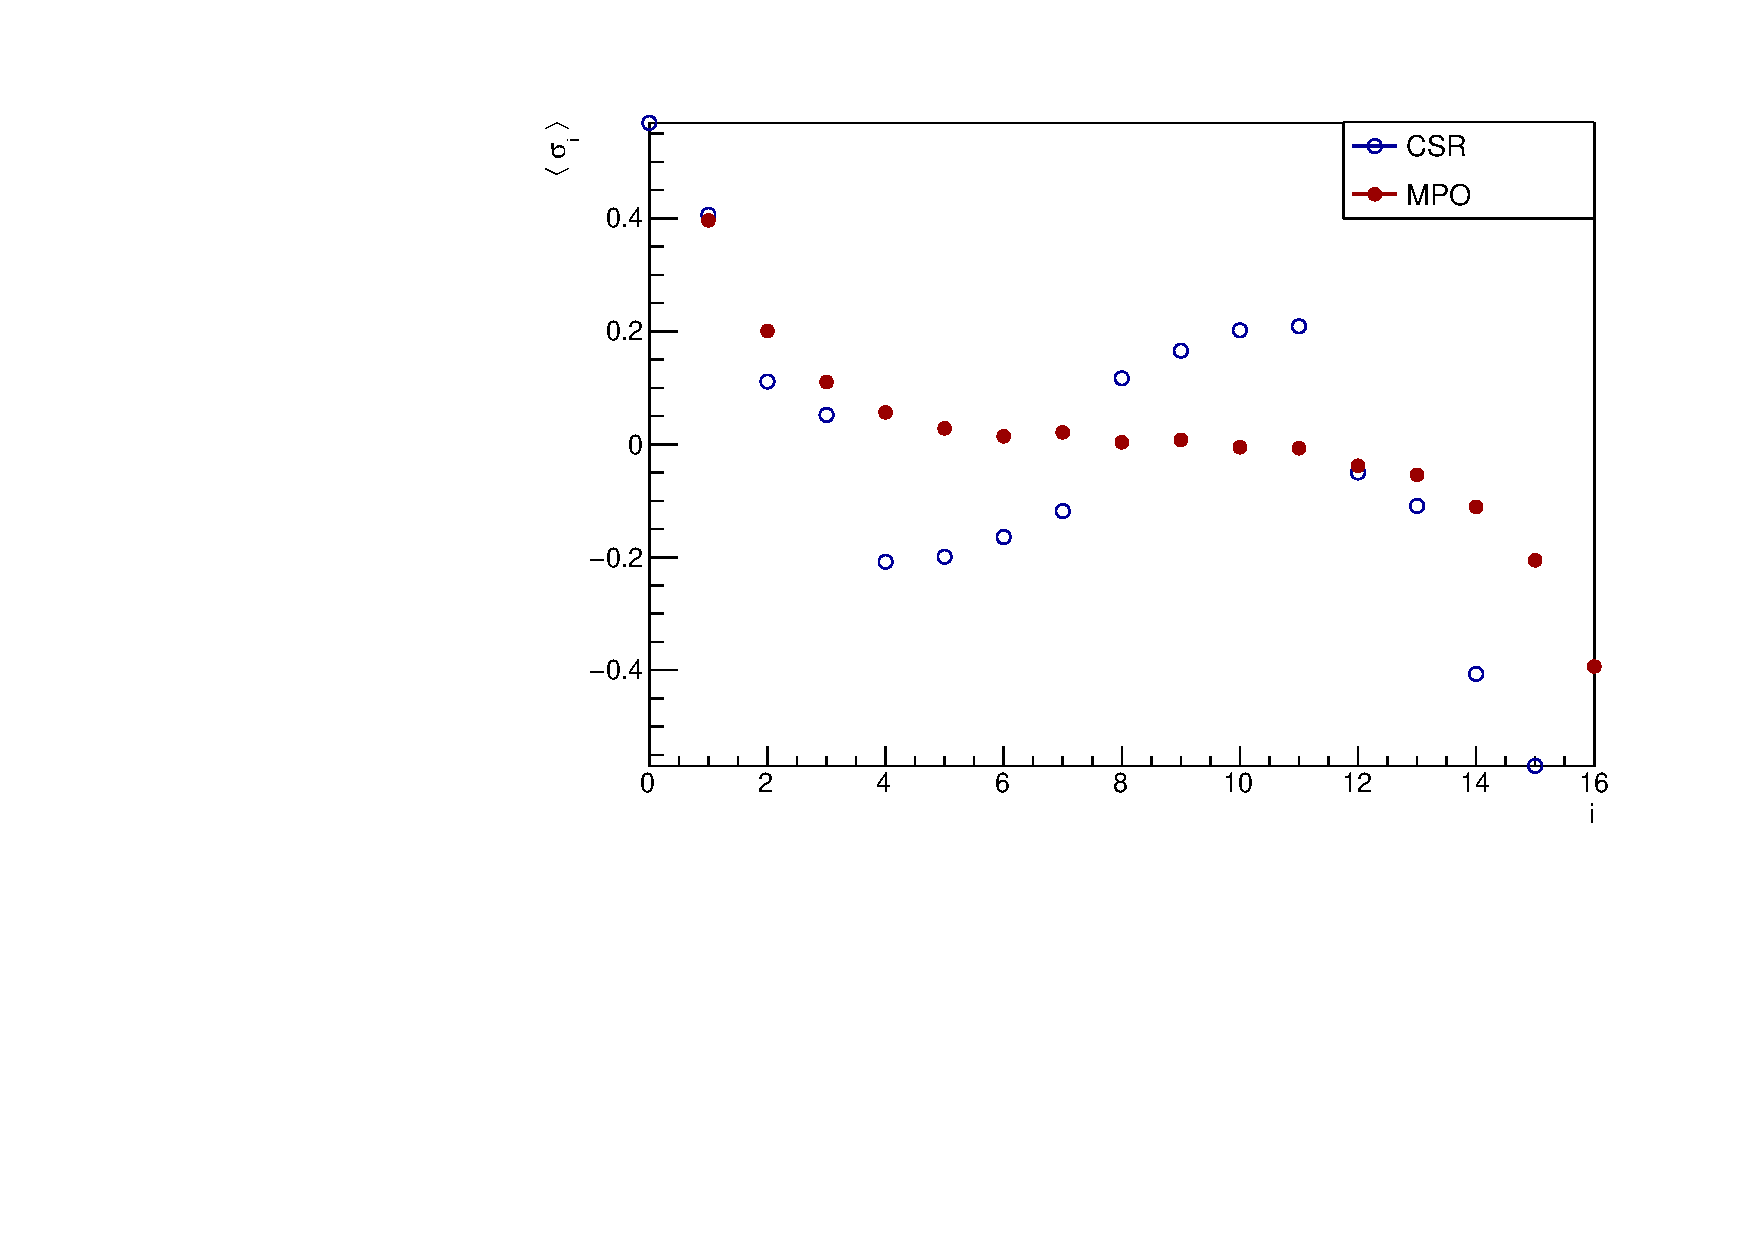
\includegraphics[scale=0.7]{Figures/16sites/LMComparison16s1051.pdf}
    \caption{Spin profile for a 16-sites chain characterized by $\gamma~=~1, J_x=1, J_y=0.5, J_z=1.5$. Data in red are obtained from MPO method, with m = 80 and T = 2000 and data in blue are obtained from CSR method, with M = 65. It is self-evident the inadequacy of the corner-space size: the complete Hilbert space for such a system has a dimension of $2^{16} \times 2^{16}$.}
    \label{fig:my_label}
\end{figure}

The following figure shows the spin profile for the model at $J_z = 1$. 

\begin{figure}[H]
    \centering
    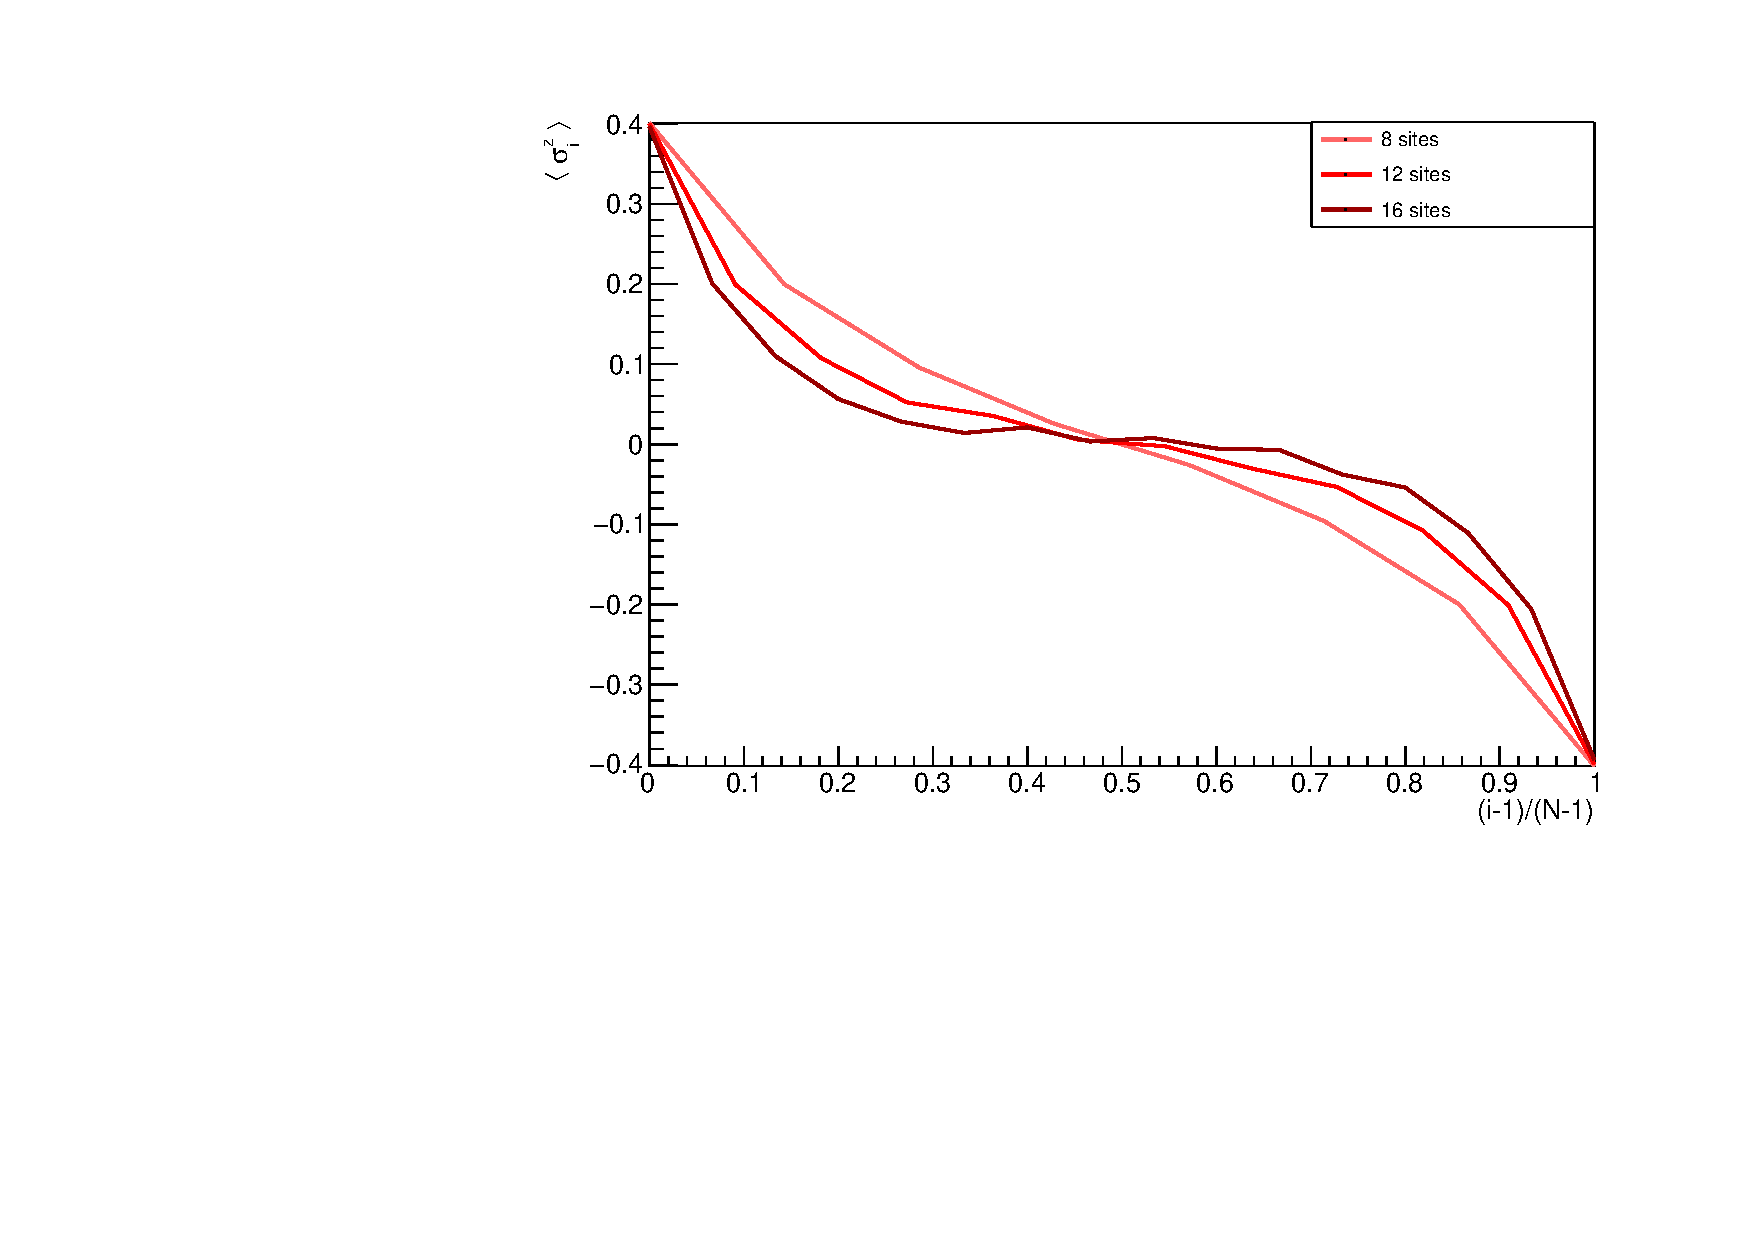
\includegraphics[scale=0.7]{Figures/NORM_LM_comparisonVSsize.pdf}
    \caption{Spin profile for the model under study at $J_z = 1$ and $\gamma=1$. Data for different chain length are shown and they are obtained from MPO method.}
    \label{fig:my_label}
\end{figure}

\begin{figure}[H]
    \centering
    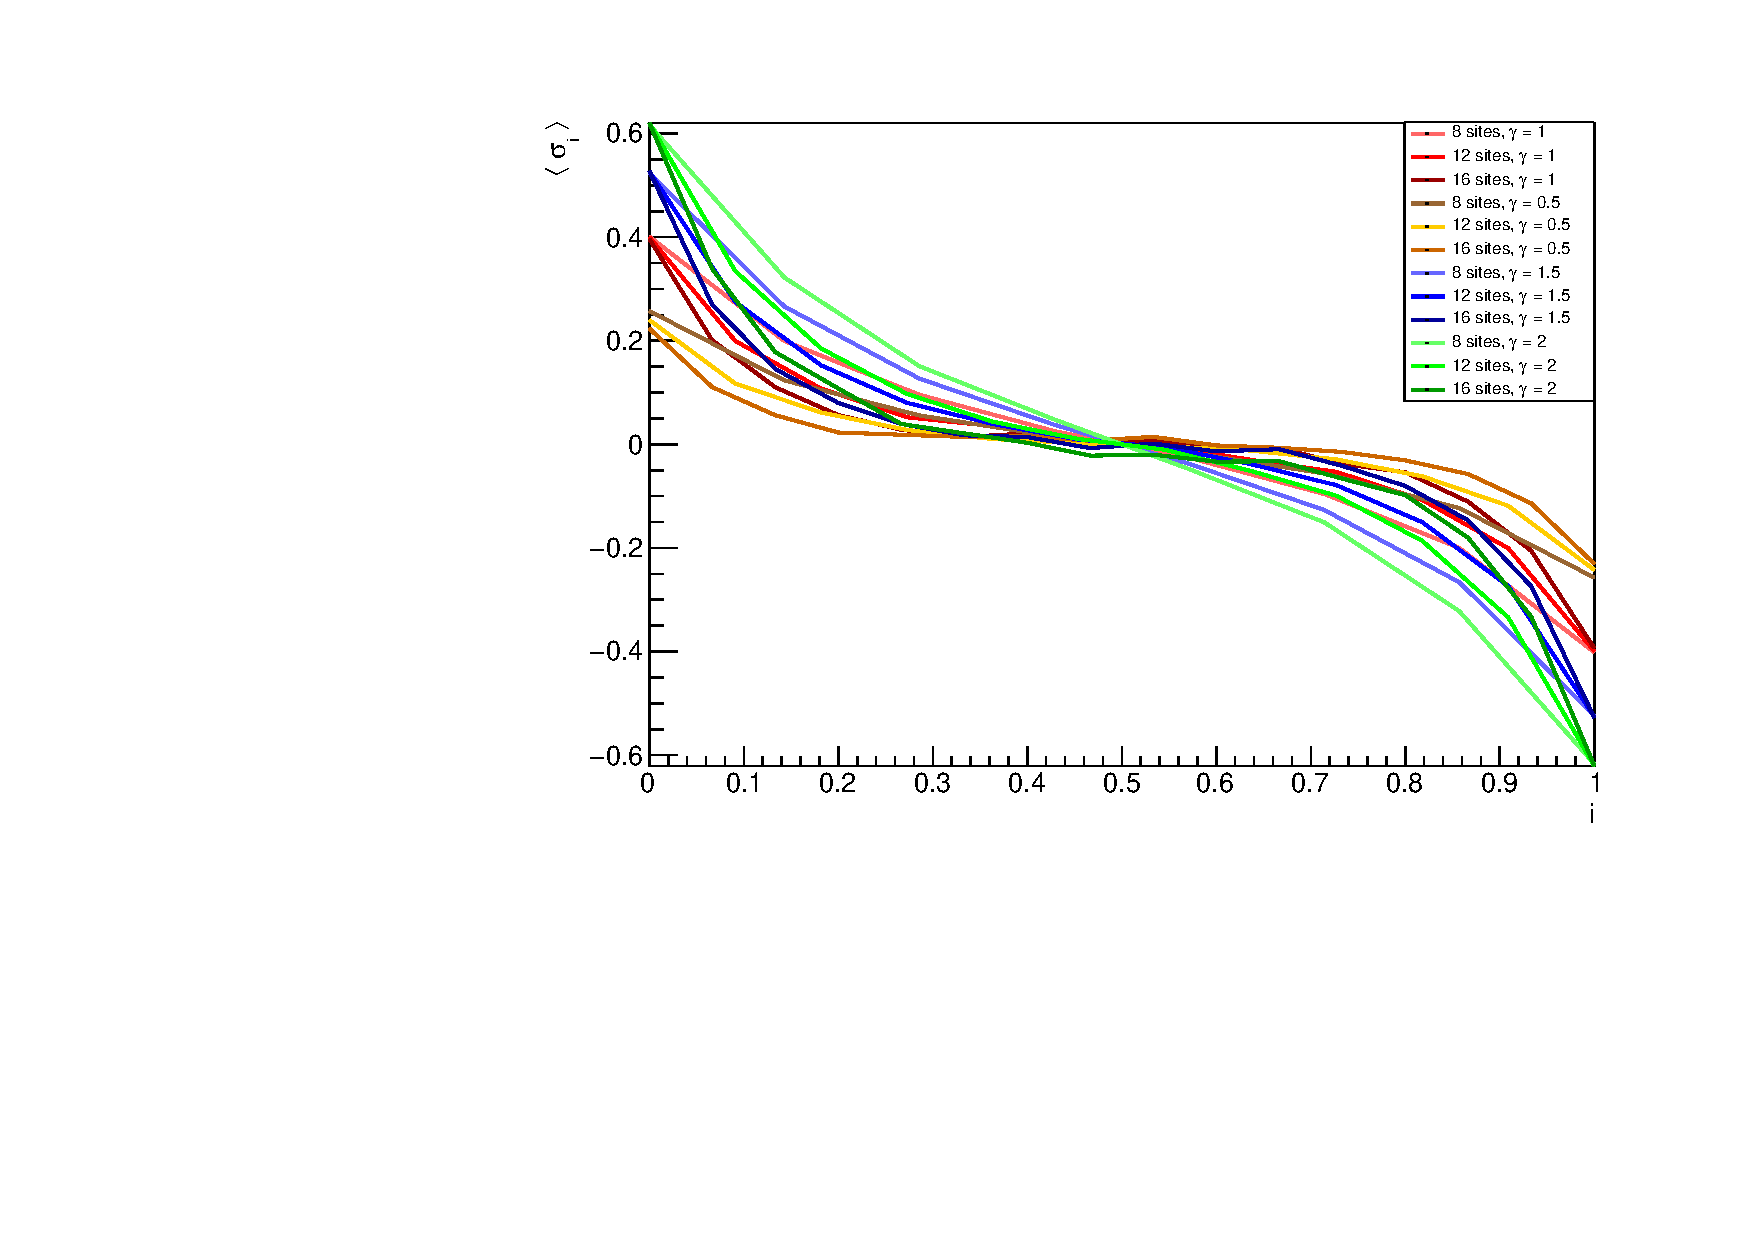
\includegraphics[scale=0.7]{Figures/LMcomparisonVSsizeANDdissipationRate.pdf}
    \caption{Spin profile for the model under study at $J_z = 1$ for several values of dissipation rate $\gamma$. It seems clear that while $\gamma$ decreases the profile gets flatter. Data are obtained from MPO method.}
    \label{fig:LMcompVSsizeANDdissRate}
\end{figure}

Now let us study in greater detail this curves. In particular we can see in figure~\ref{fig:LMcompVSsizeANDdissRate} that the peak of the $\langle \sigma^z \rangle$ in the first site due to the presence of dissipator $\sigma^+$, increases while the value of dissipation rate $\gamma$ grows. In the following, we will see how.

\begin{figure}[H]
    \centering
    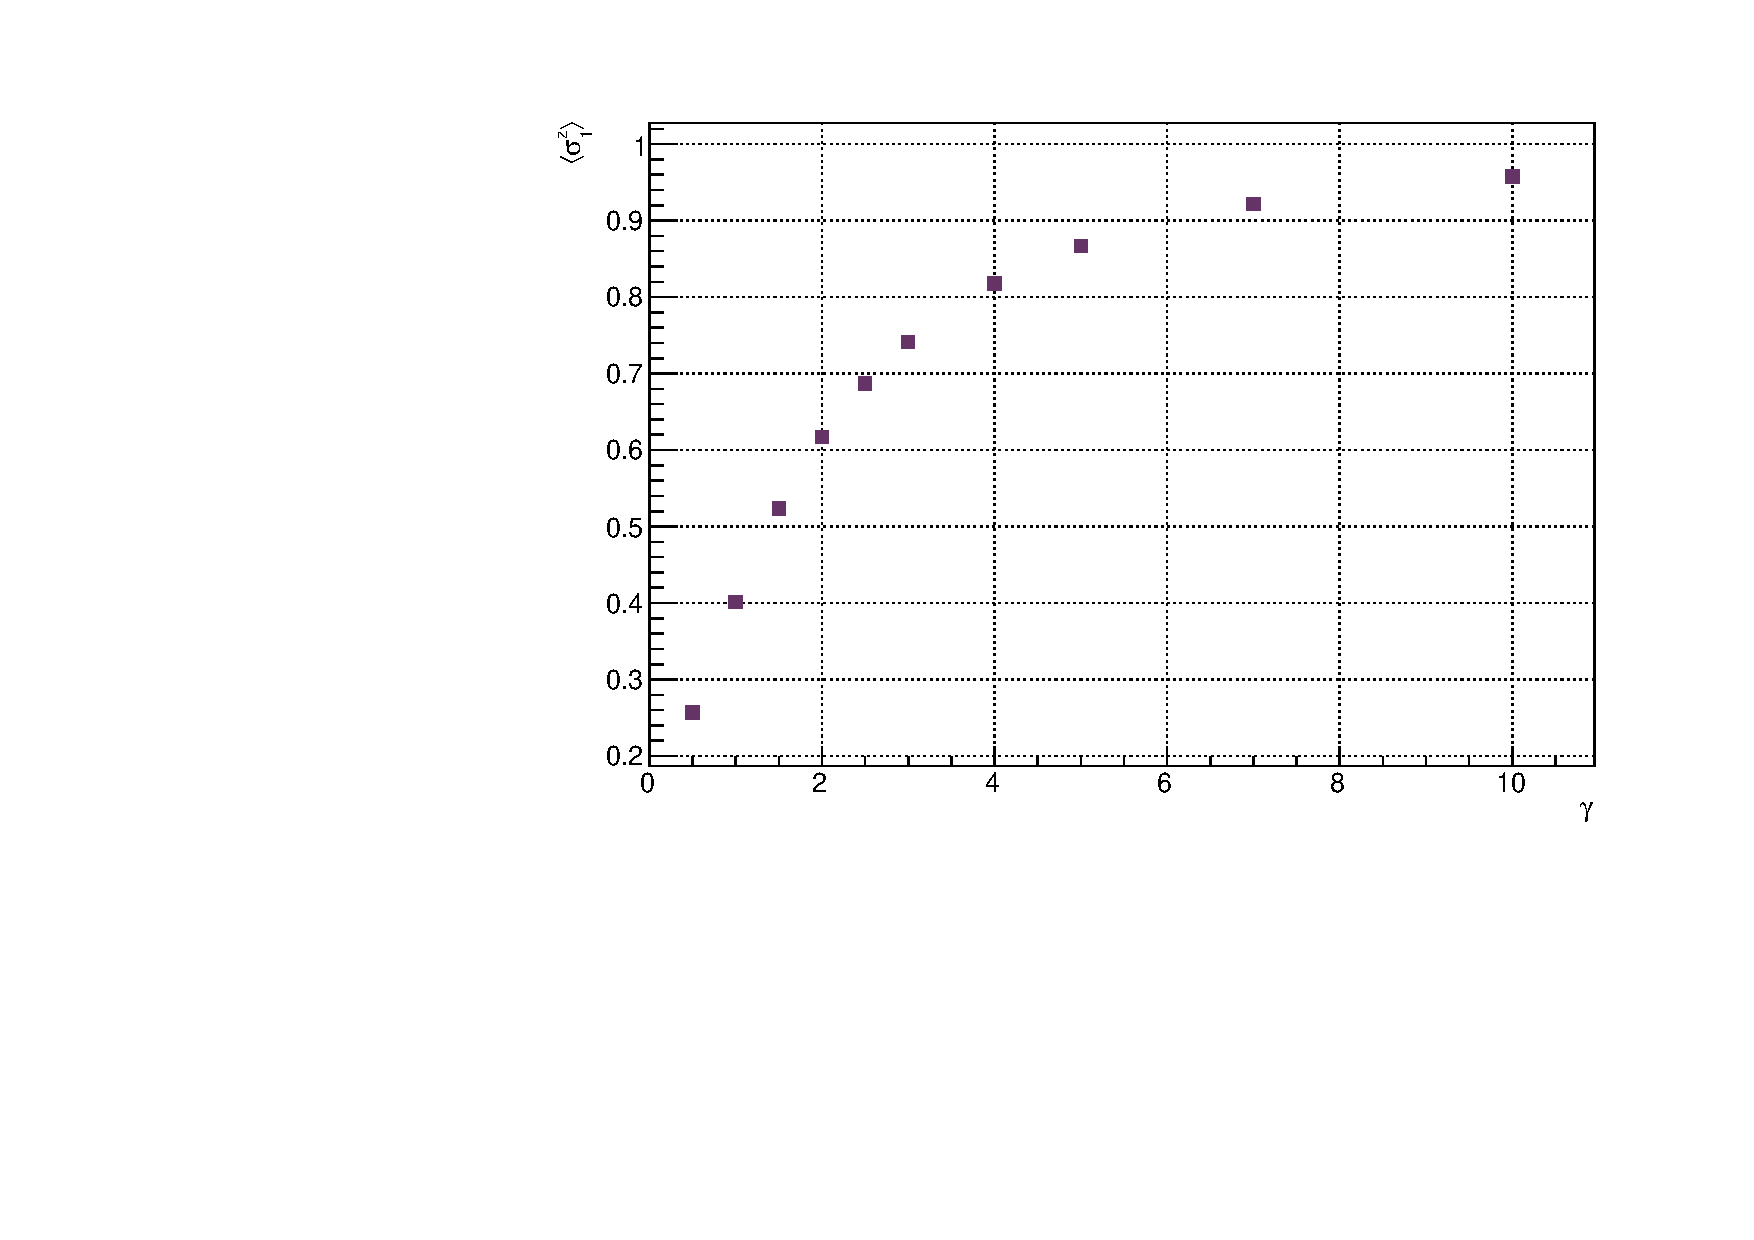
\includegraphics[scale=0.8]{Figures/8sites_PeakLMvsGamma_J1051.pdf}
    \caption{Caption}
    \label{fig:PeakLMvsGamma_J1051}
\end{figure}


%%%%%%%%%%%%%%%%%%%%%%%%%%%%%%%%%%%%%%%%%%%%%%%%%%%%%%%%%%%%%%%%%%
%%%%%%%%%%%%%%%%%%%%%%%%%%%%%%%%%%%%%%%%%%%%%%%%%%%%%%%%%%%%%%%%%%
%%%%%%%%%%%%%%%%%%%%%%%%%%%%%%%%%%%%%%%%%%%%%%%%%%%%%%%%%%%%%%%%%%
\section{Two-Points Correlation Functions}
As said previously, we are interested in the behaviour of the spins in the chain and how much they are influenced by the presence of the others. In order to analyze this aspect, we are going to study the two-point correlation function with respect to the first and the last site and the \emph{bulk} correlation function.

First of all, as done in the last section, let us see if the results of each method retrace the ones of the other two, for the case of 8-sites chain. 

\begin{figure}[H]
    \centering
    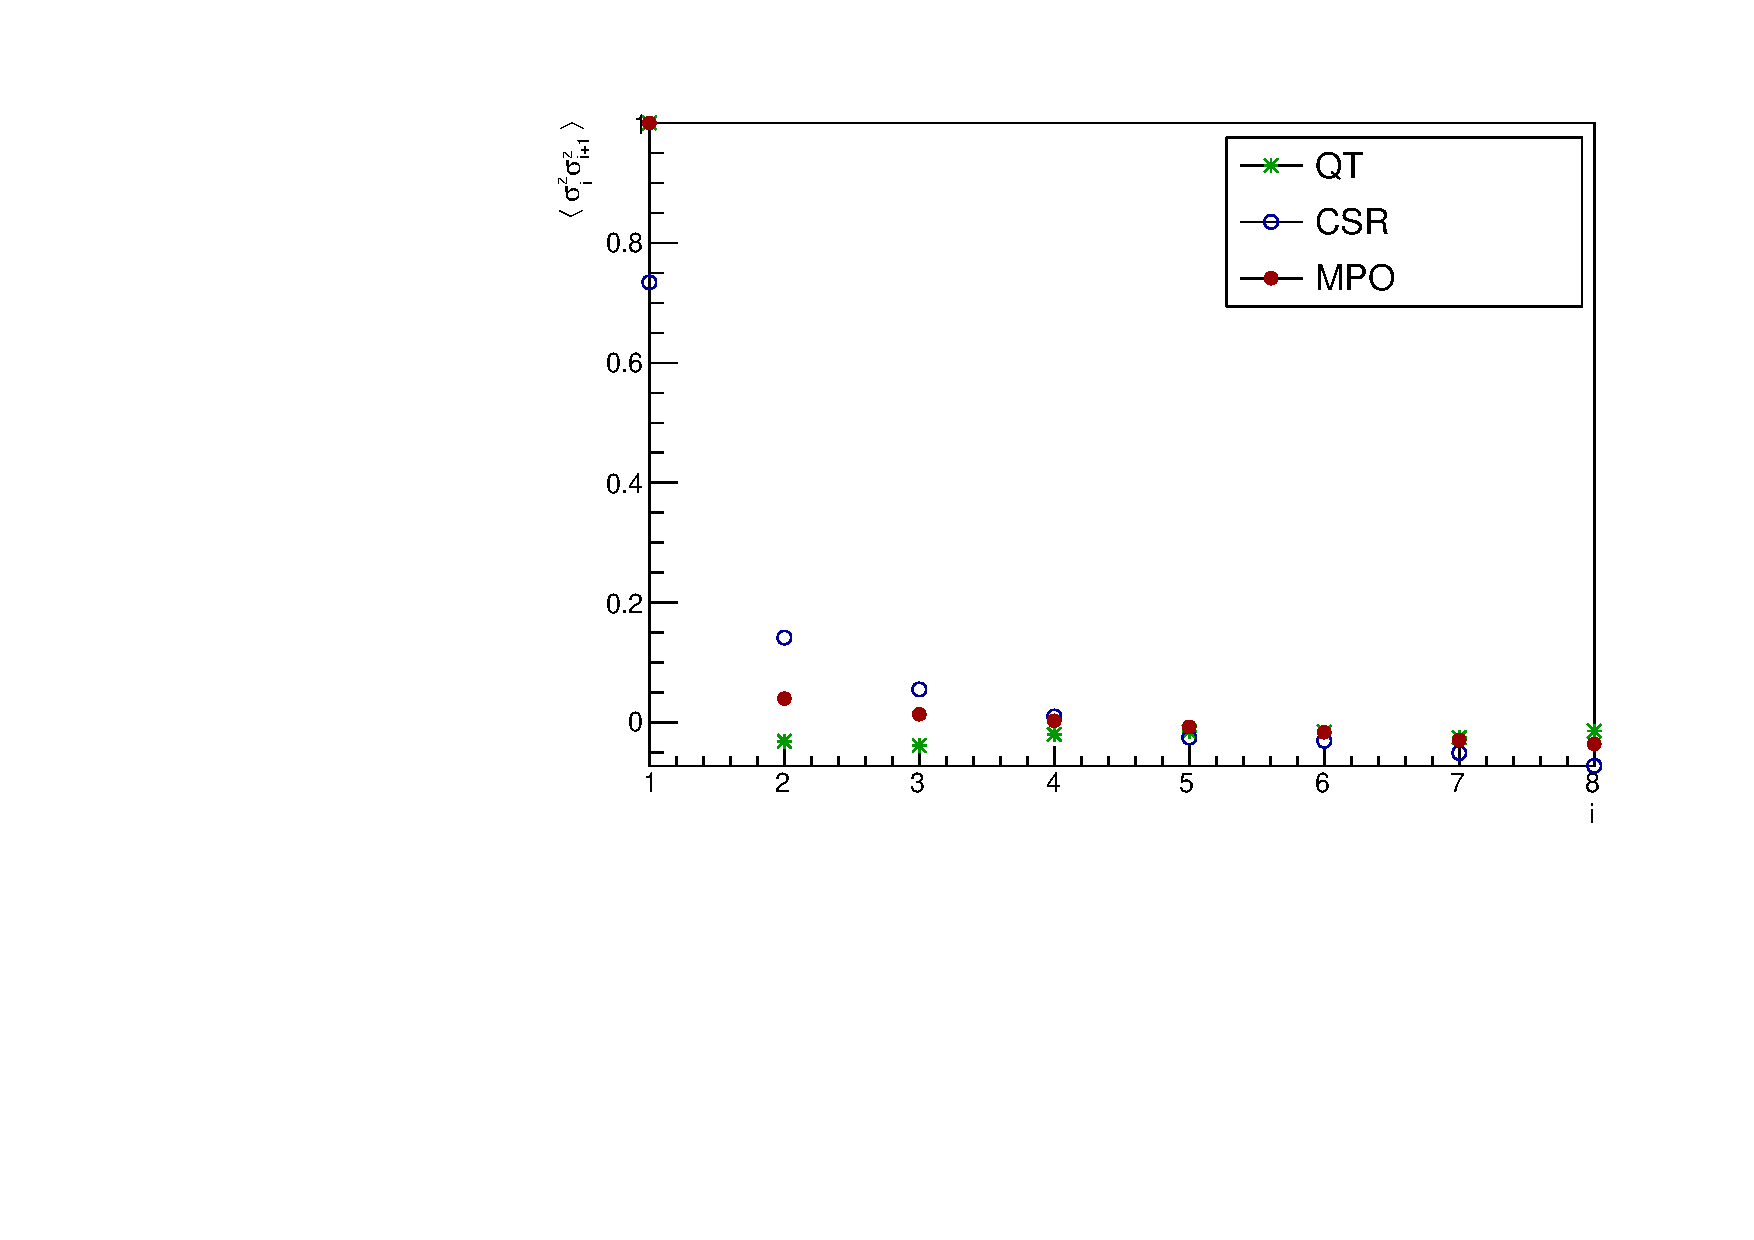
\includegraphics[scale=0.7]{Figures/8sites_comparison/CorrFunc1_8s_J10505.pdf}
    \caption{Correlation function with respect to the spin positioned in the first site of the chain, characterized by $\gamma~=~1, J_x=1, J_y=0.5, J_z=0.5$; \emph{i} stands for the site index.}
    \label{fig:my_label}
\end{figure}

\begin{figure}[H]
    \centering
    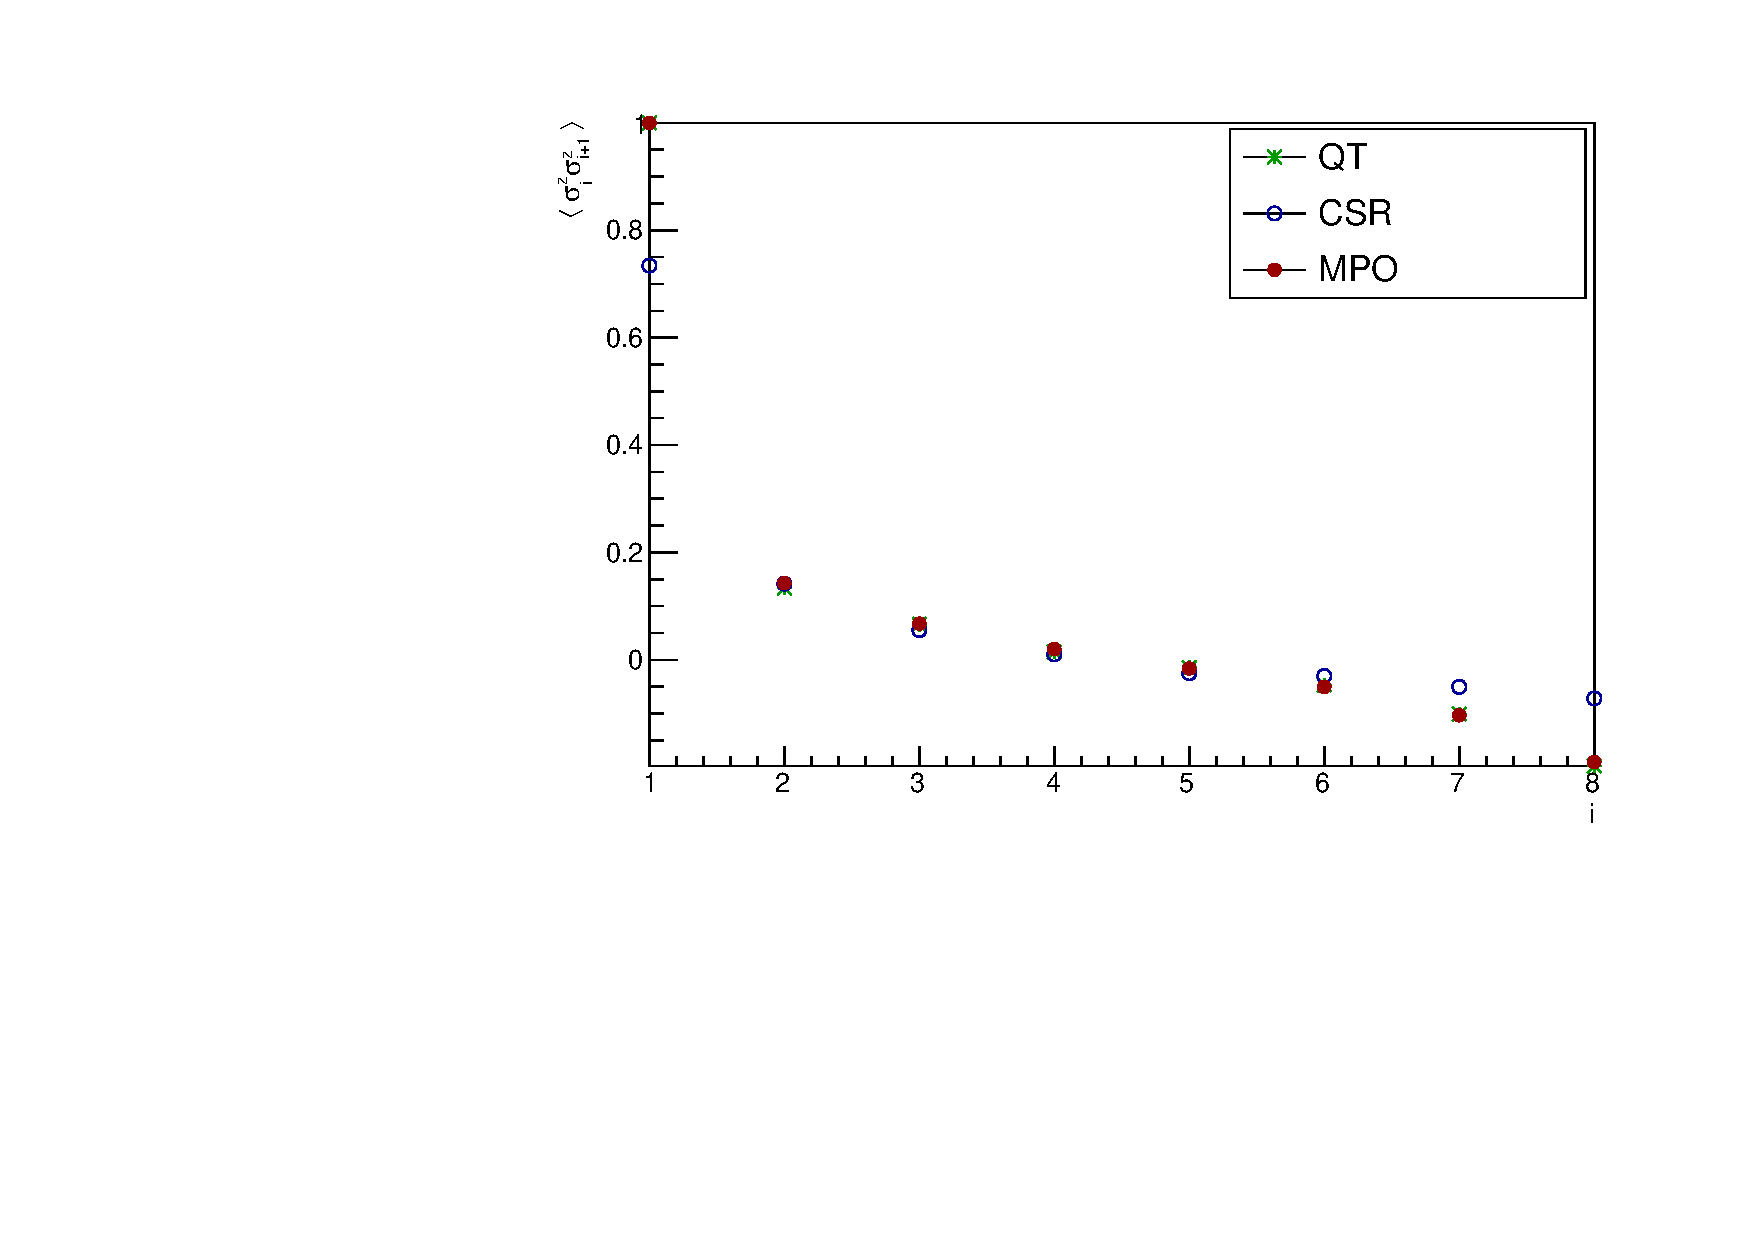
\includegraphics[scale=0.7]{Figures/8sites_comparison/CorrFunc1_8s_J1051.pdf}
    \caption{Correlation function with respect to the spin positioned in the first site of the chain, characterized by $\gamma~=~1, J_x=1, J_y=0.5, J_z=1$; \emph{i} stands for the site index.}
    \label{fig:my_label}
\end{figure}

\begin{figure}[H]
    \centering
    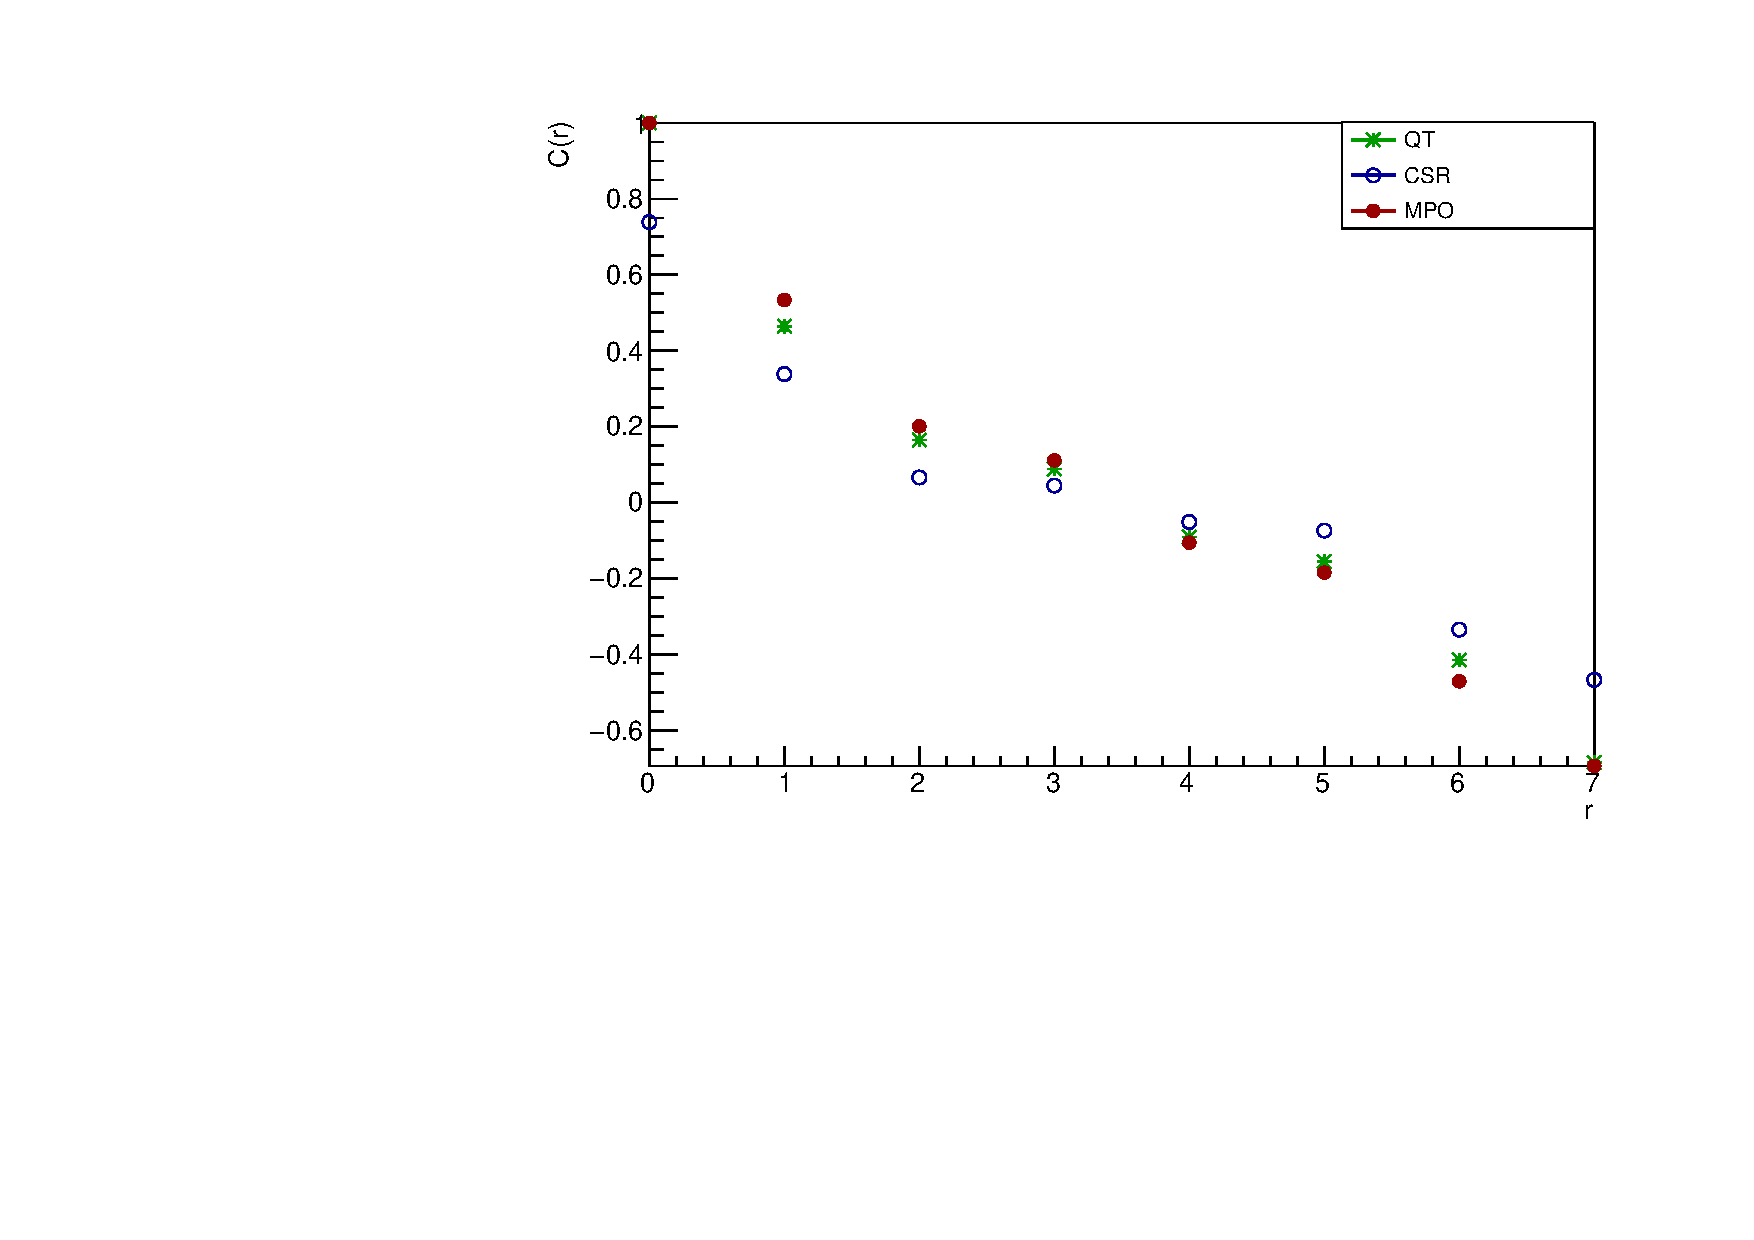
\includegraphics[scale=0.7]{Figures/8sites_comparison/CorrFunc1_8s_J10515.pdf}
    \caption{Correlation function with respect to the spin positioned in the first site of the chain, characterized by $\gamma~=~1, J_x=1, J_y=0.5, J_z=1.5$; \emph{i} stands for the site index.}
    \label{fig:my_label}
\end{figure}

It is interesting how the profile of correlation changes from an exponential behaviour to a linear one. In the following, we will see how this linear profile changes with respect to $\Delta$. The following fits, as all those performed in this thesis, are done by~\cite{root_cern}.

\begin{figure}[H]
    \centering
    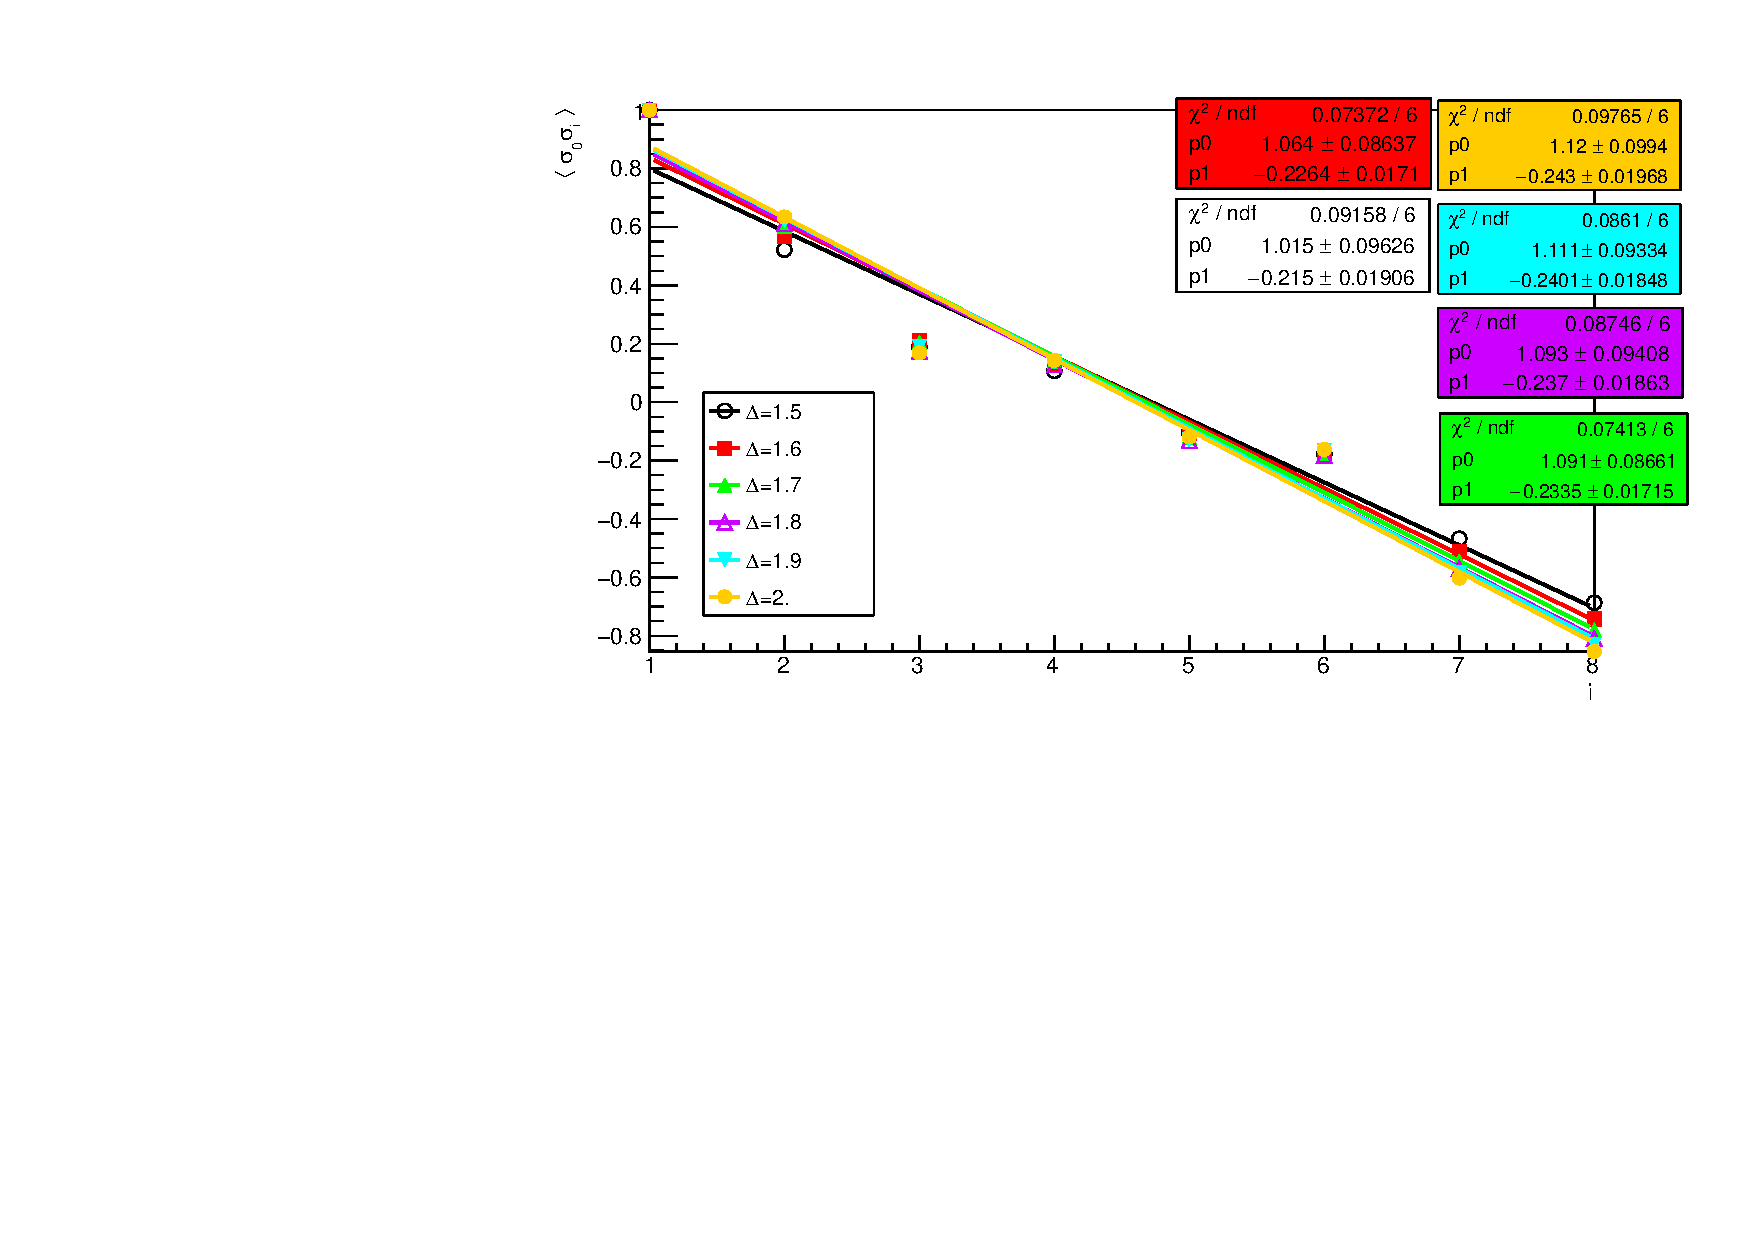
\includegraphics[scale=0.8]{Figures/8sites_comparison/FIT8sCorrFunc1_MPO_over15.pdf}
    \caption{Data are obtained from QT method.}
    \label{fig:my_label}
\end{figure}

It is interesting to analyze the so-called \emph{bulk} correlation function. 

\begin{figure}[H]
    \centering
    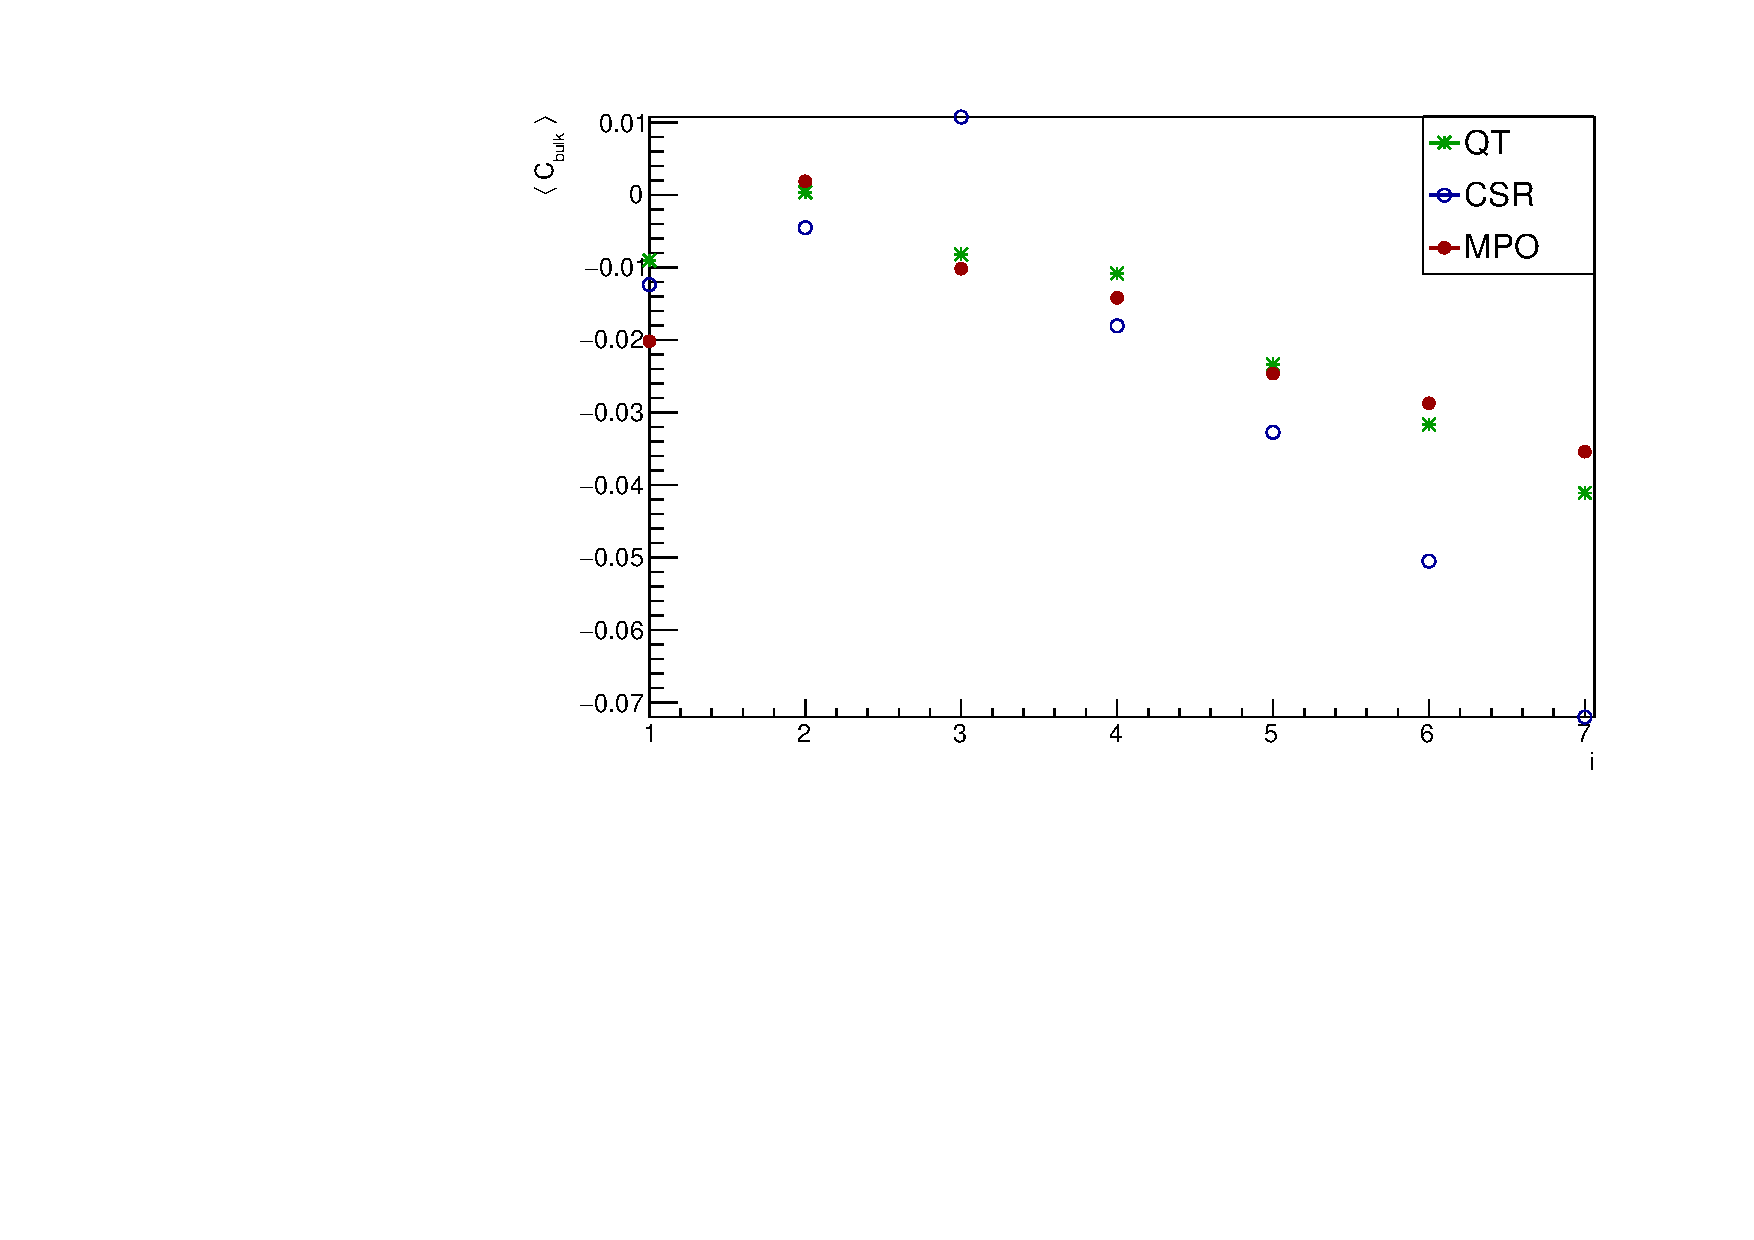
\includegraphics[scale=0.7]{Figures/8sites_comparison/CorrFuncBulk_8sJ10505.pdf}
    \caption{Bulk correlation function for a 8-sites chain characterized by $\gamma~=~1, J_x=1, J_y=0.5, J_z=0.5$.}
    \label{fig:my_label}
\end{figure}

\begin{figure}[H]
    \centering
    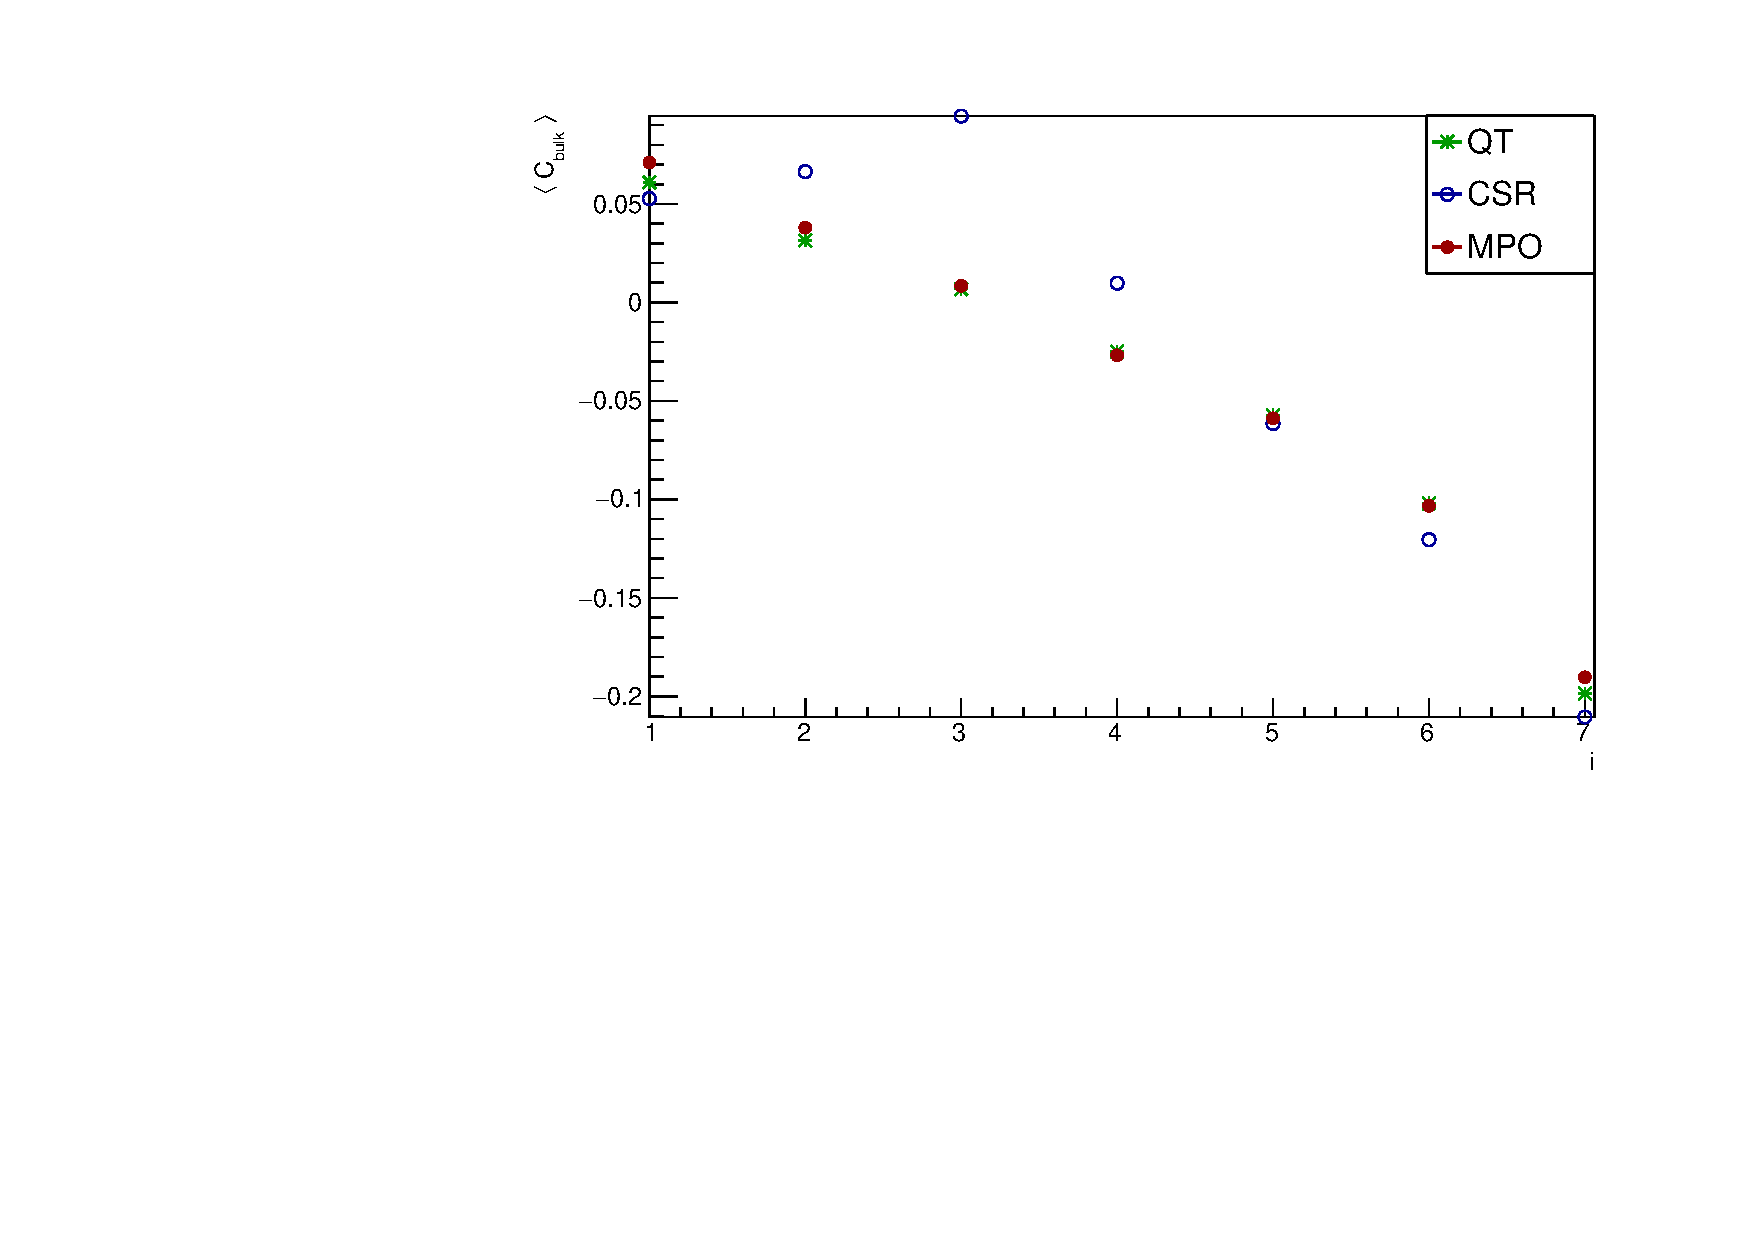
\includegraphics[scale=0.7]{Figures/8sites_comparison/CorrFuncBulk_8sJ1051.pdf}
    \caption{Bulk correlation function for a 8-sites chain characterized by $\gamma~=~1, J_x=1, J_y=0.5, J_z=1$.}
    \label{fig:my_label}
\end{figure}

\begin{figure}[H]
    \centering
    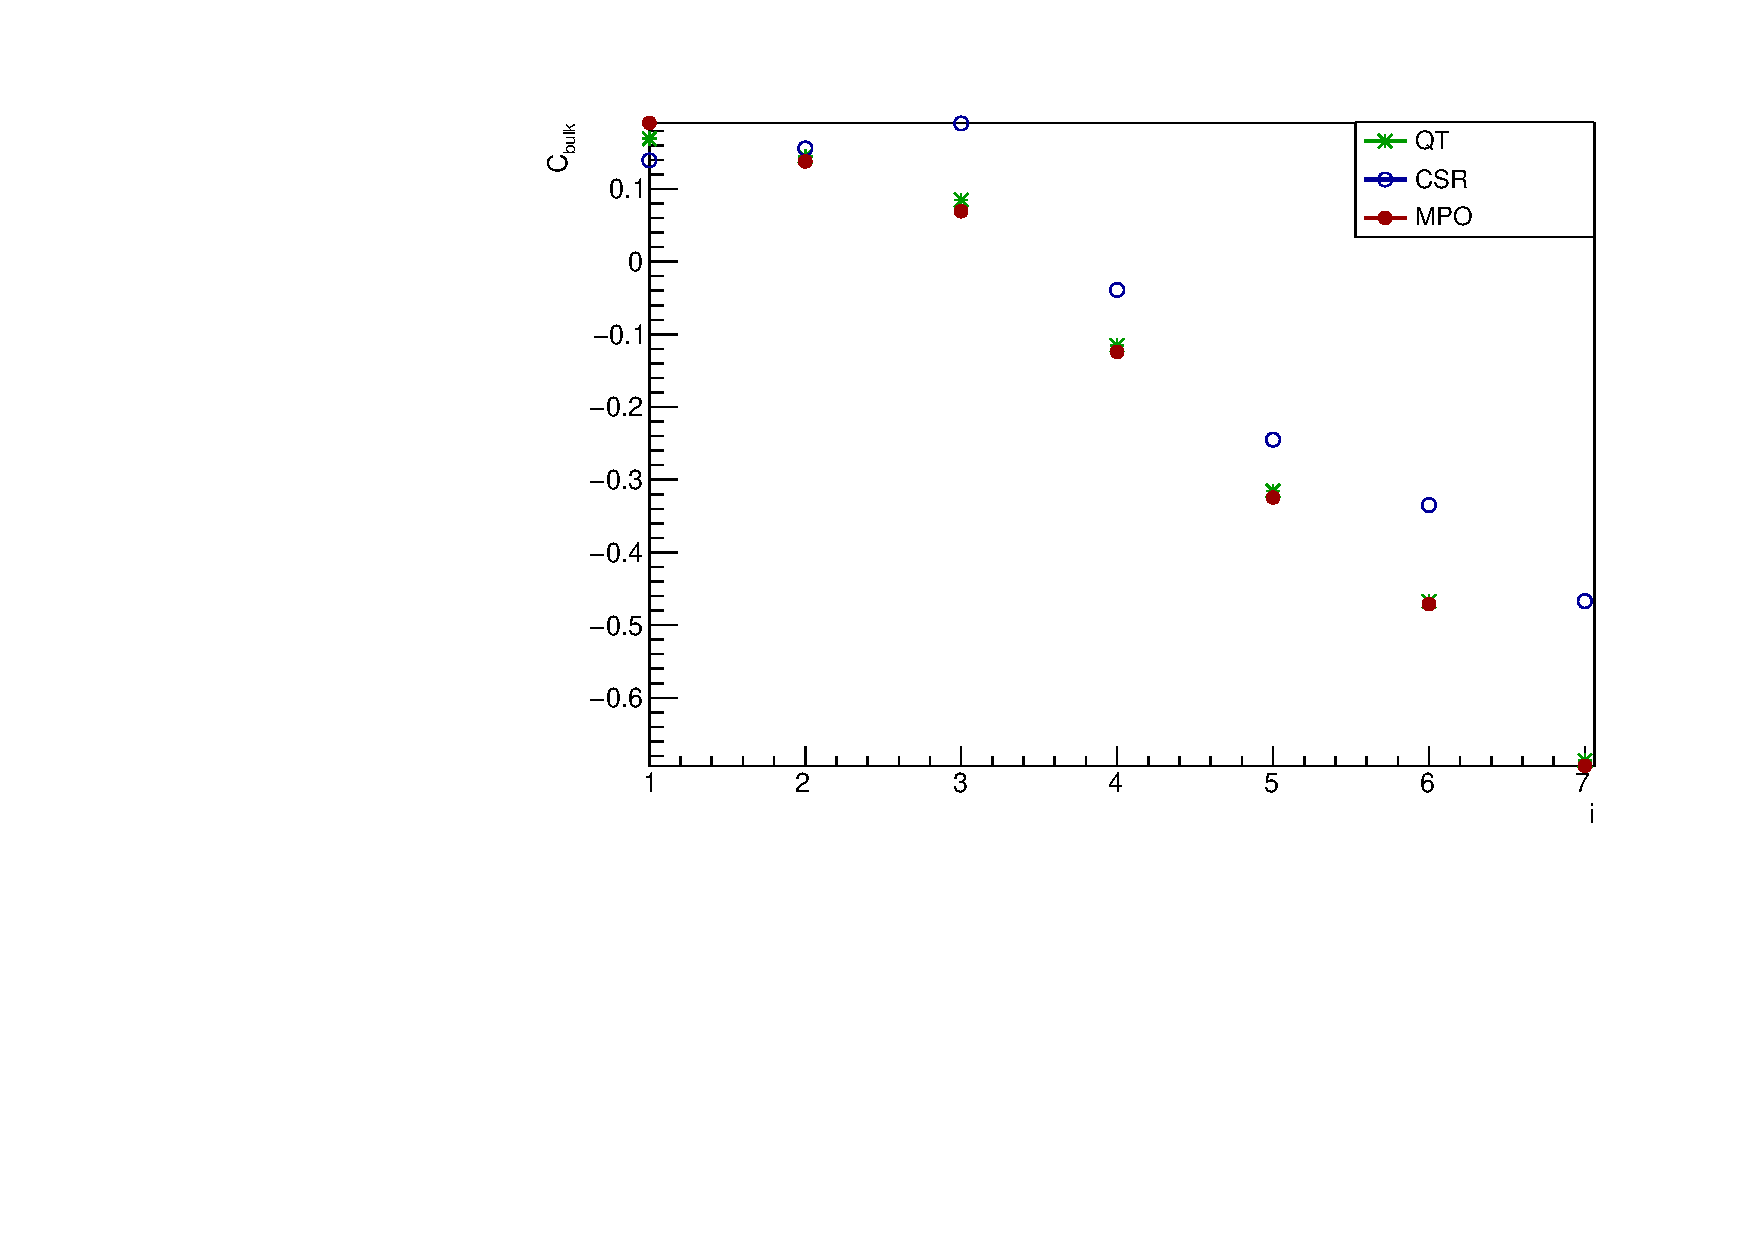
\includegraphics[scale=0.7]{Figures/8sites_comparison/CorrFuncBulk_8sJ10515.pdf}
    \caption{Bulk correlation function for a 8-sites chain characterized by $\gamma~=~1, J_x=1, J_y=0.5, J_z=1.5$.}
    \label{fig:my_label}
\end{figure}

%%%%%%%%%%%%%%%%%%%%%%%%%%%%%%%%%%%%%%%%%%%%%%%%%%%%%%%%%%%%%%%%%%
%%%%%%%%%%%%%%%%%%%%%%%%%%%%%%%%%%%%%%%%%%%%%%%%%%%%%%%%%%%%%%%%%%
%%%%%%%%%%%%%%%%%%%%%%%%%%%%%%%%%%%%%%%%%%%%%%%%%%%%%%%%%%%%%%%%%%
\section{Spin Transport}
In this section we are going to study the spin current $j_\sigma$ defined from the continuity equation for the local spin operators~\cite{BenentiCasatiProsenRossini}:
\begin{equation}
    \frac{\partial S^k_z}{\partial t} + \nabla (j_\sigma)_k = 0,
\end{equation}
which can be rewritten as
\begin{equation}
    (j_\sigma)_{k+1}-(j_\sigma)_k = \frac{i}{2}[\sigma_k^z , H],
\end{equation}
where $S_k^z \equiv \sigma_k^z/2$ and where $H$ is the Hamiltonian written in~\ref{ham_chain}. So, we obtain:
\begin{equation}
    j_\sigma = J_y (\sigma_k^x \sigma_{k+1}^y) - J_x (\sigma_k^y \sigma_{k+1}^x).
\end{equation}

\begin{figure}[H]
    \centering
    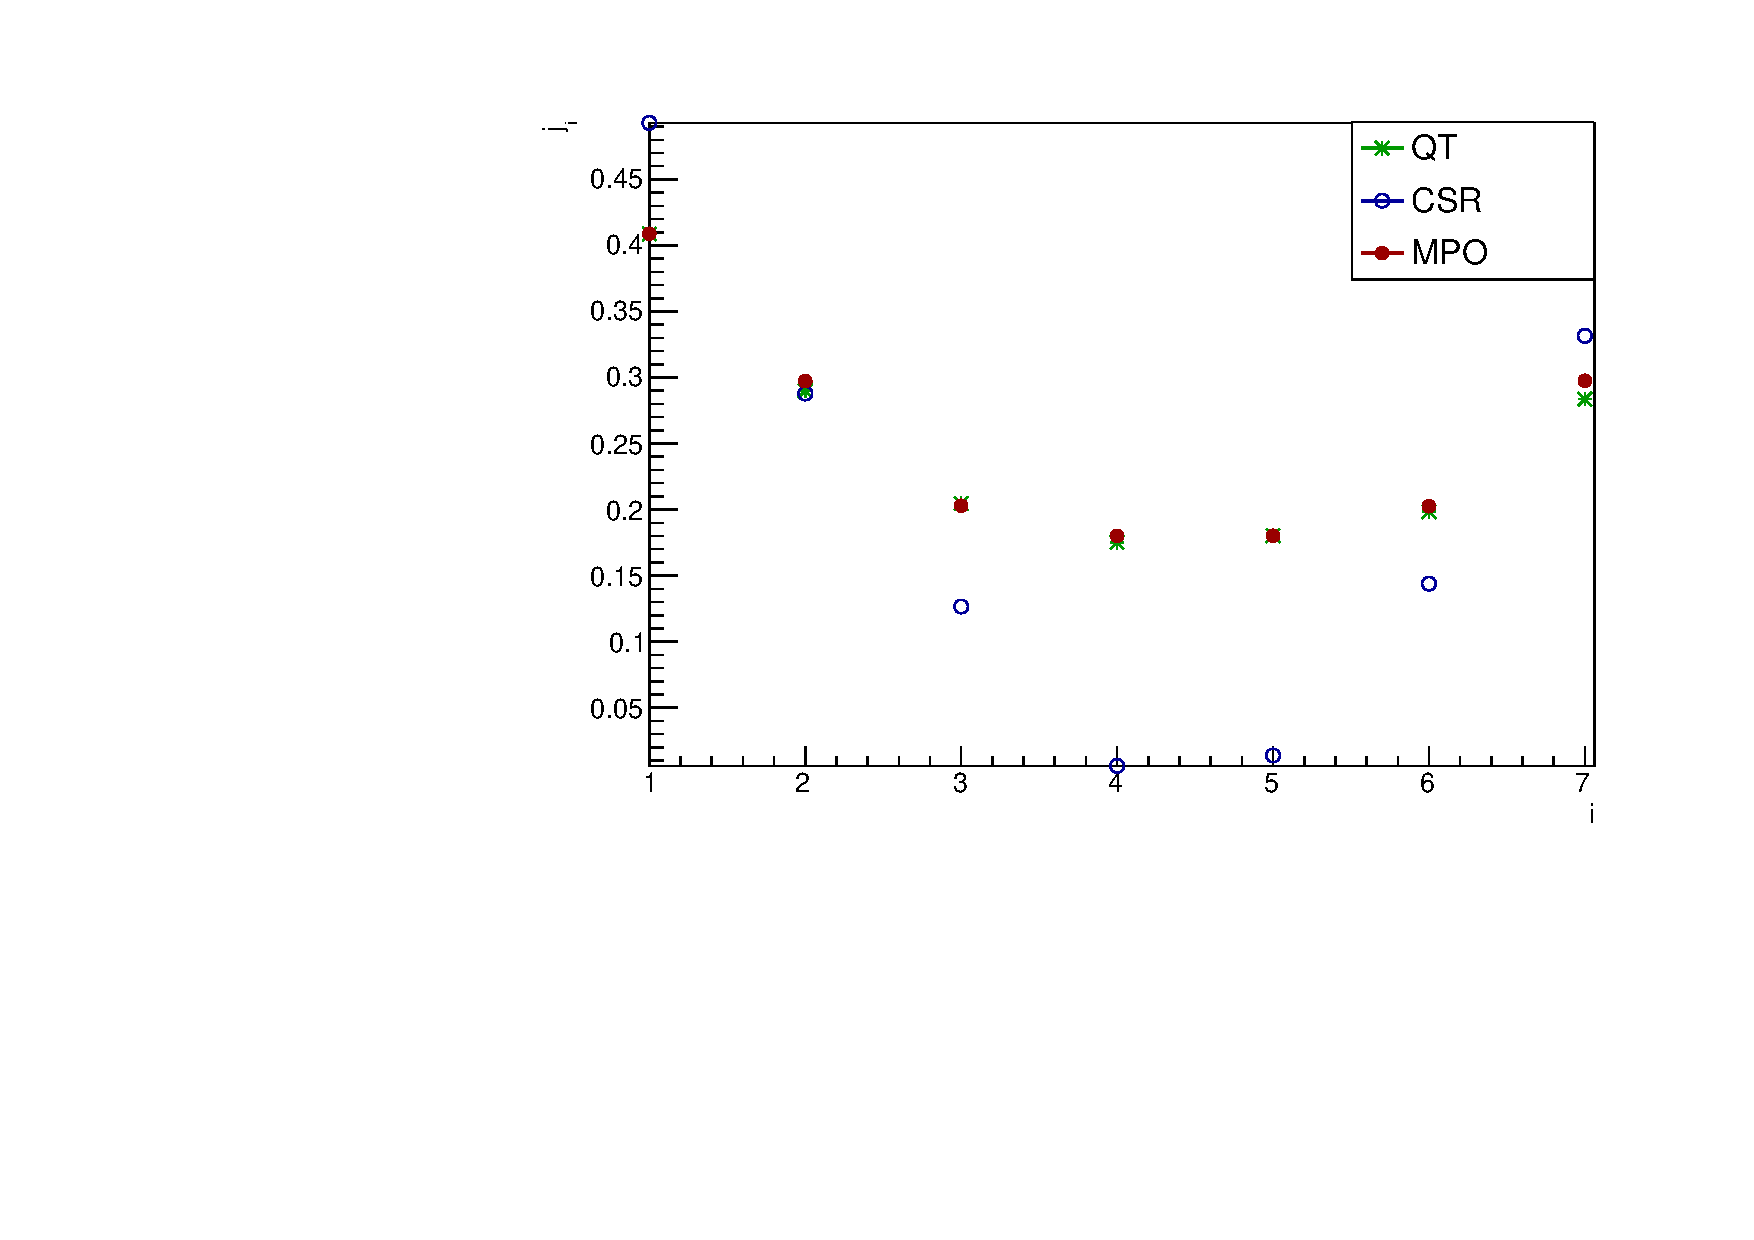
\includegraphics[scale=0.7]{Figures/8sites_comparison/SpinCurr_8s_J10505.pdf}
    \caption{Spin current of the chain, characterized by $\gamma=1, J_x=1, J_y=0.5, J_z=0.5$; \emph{i} stands for the site index.}
    \label{fig:my_label}
\end{figure}

\begin{figure}[H]
    \centering
    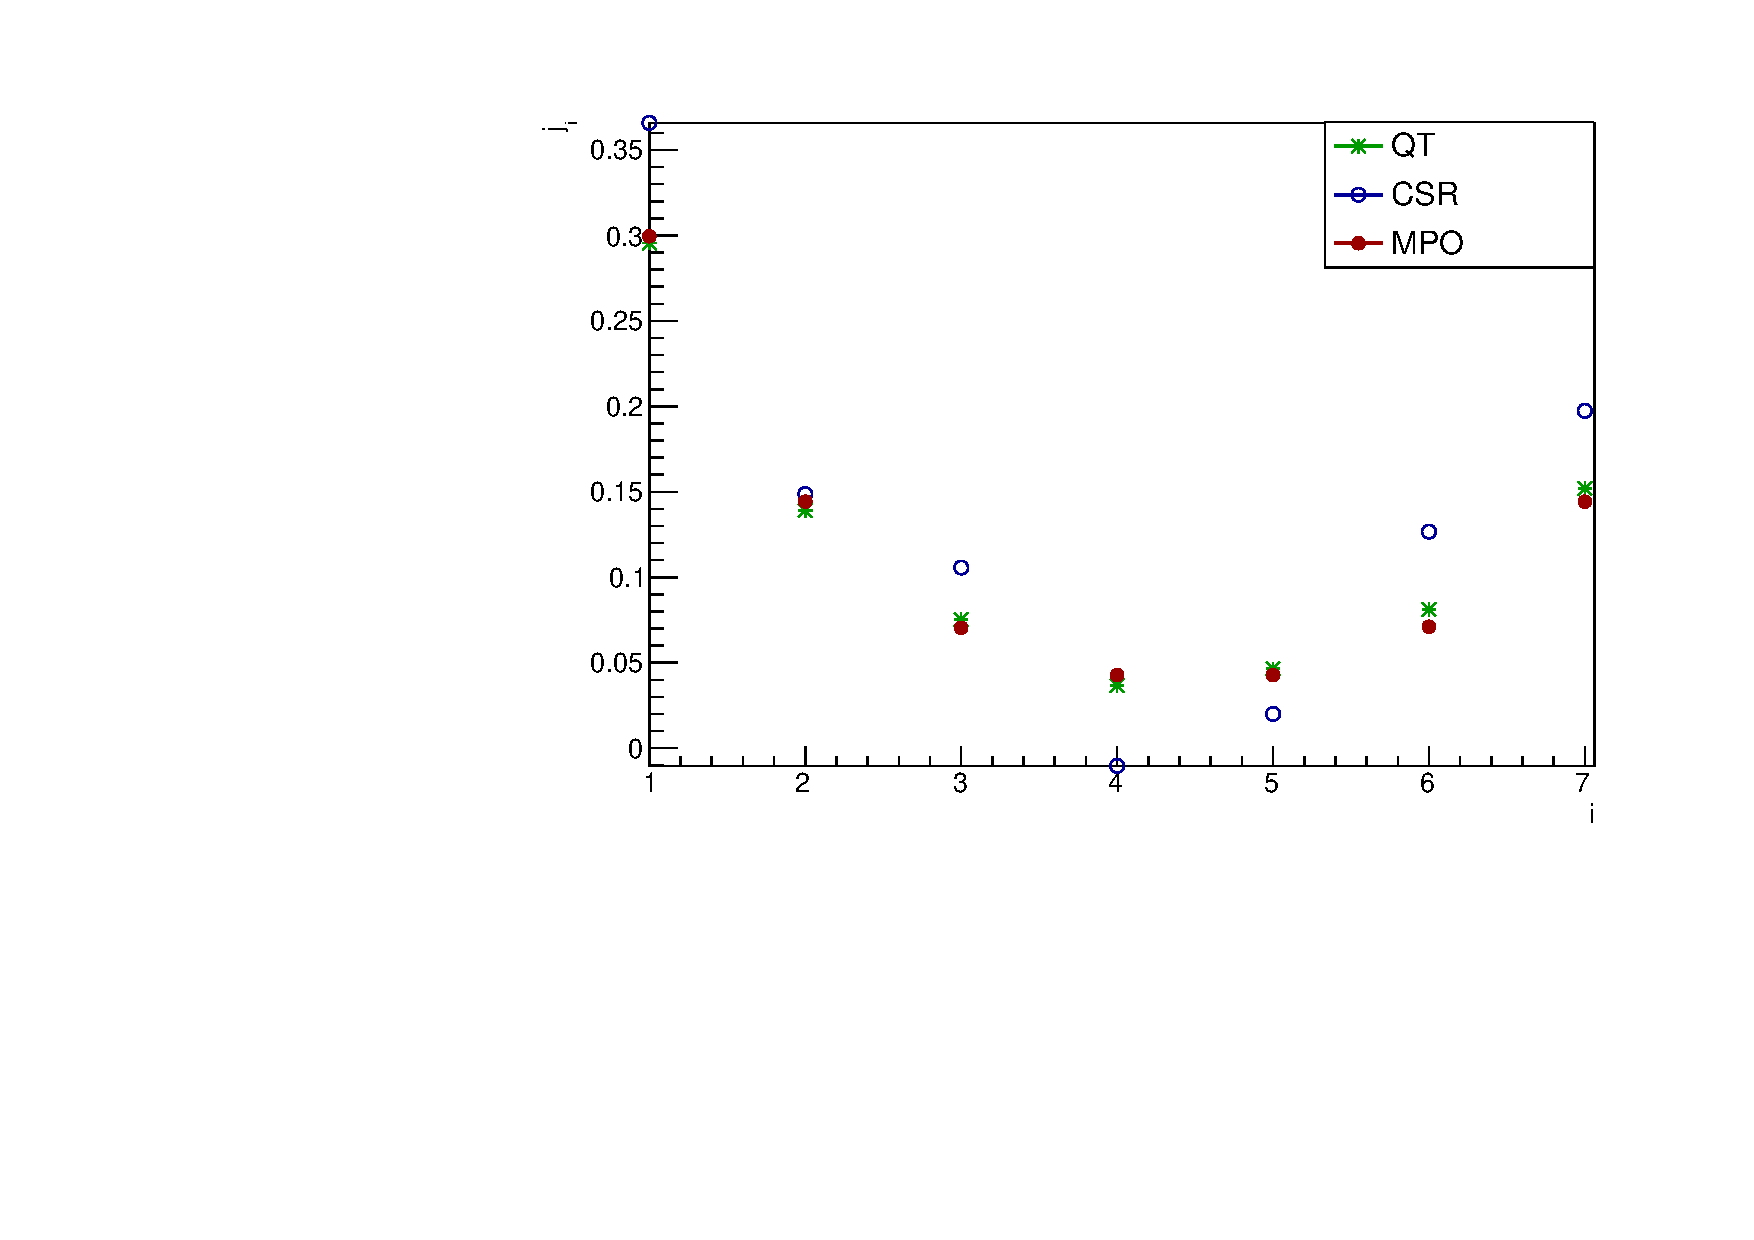
\includegraphics[scale=0.7]{Figures/8sites_comparison/SpinCurr_8s_J1051.pdf}
    \caption{Spin current of the chain, characterized by $\gamma=1, J_x=1, J_y=0.5, J_z=1$; \emph{i} stands for the site index.}
    \label{fig:my_label}
\end{figure}

\begin{figure}[H]
    \centering
    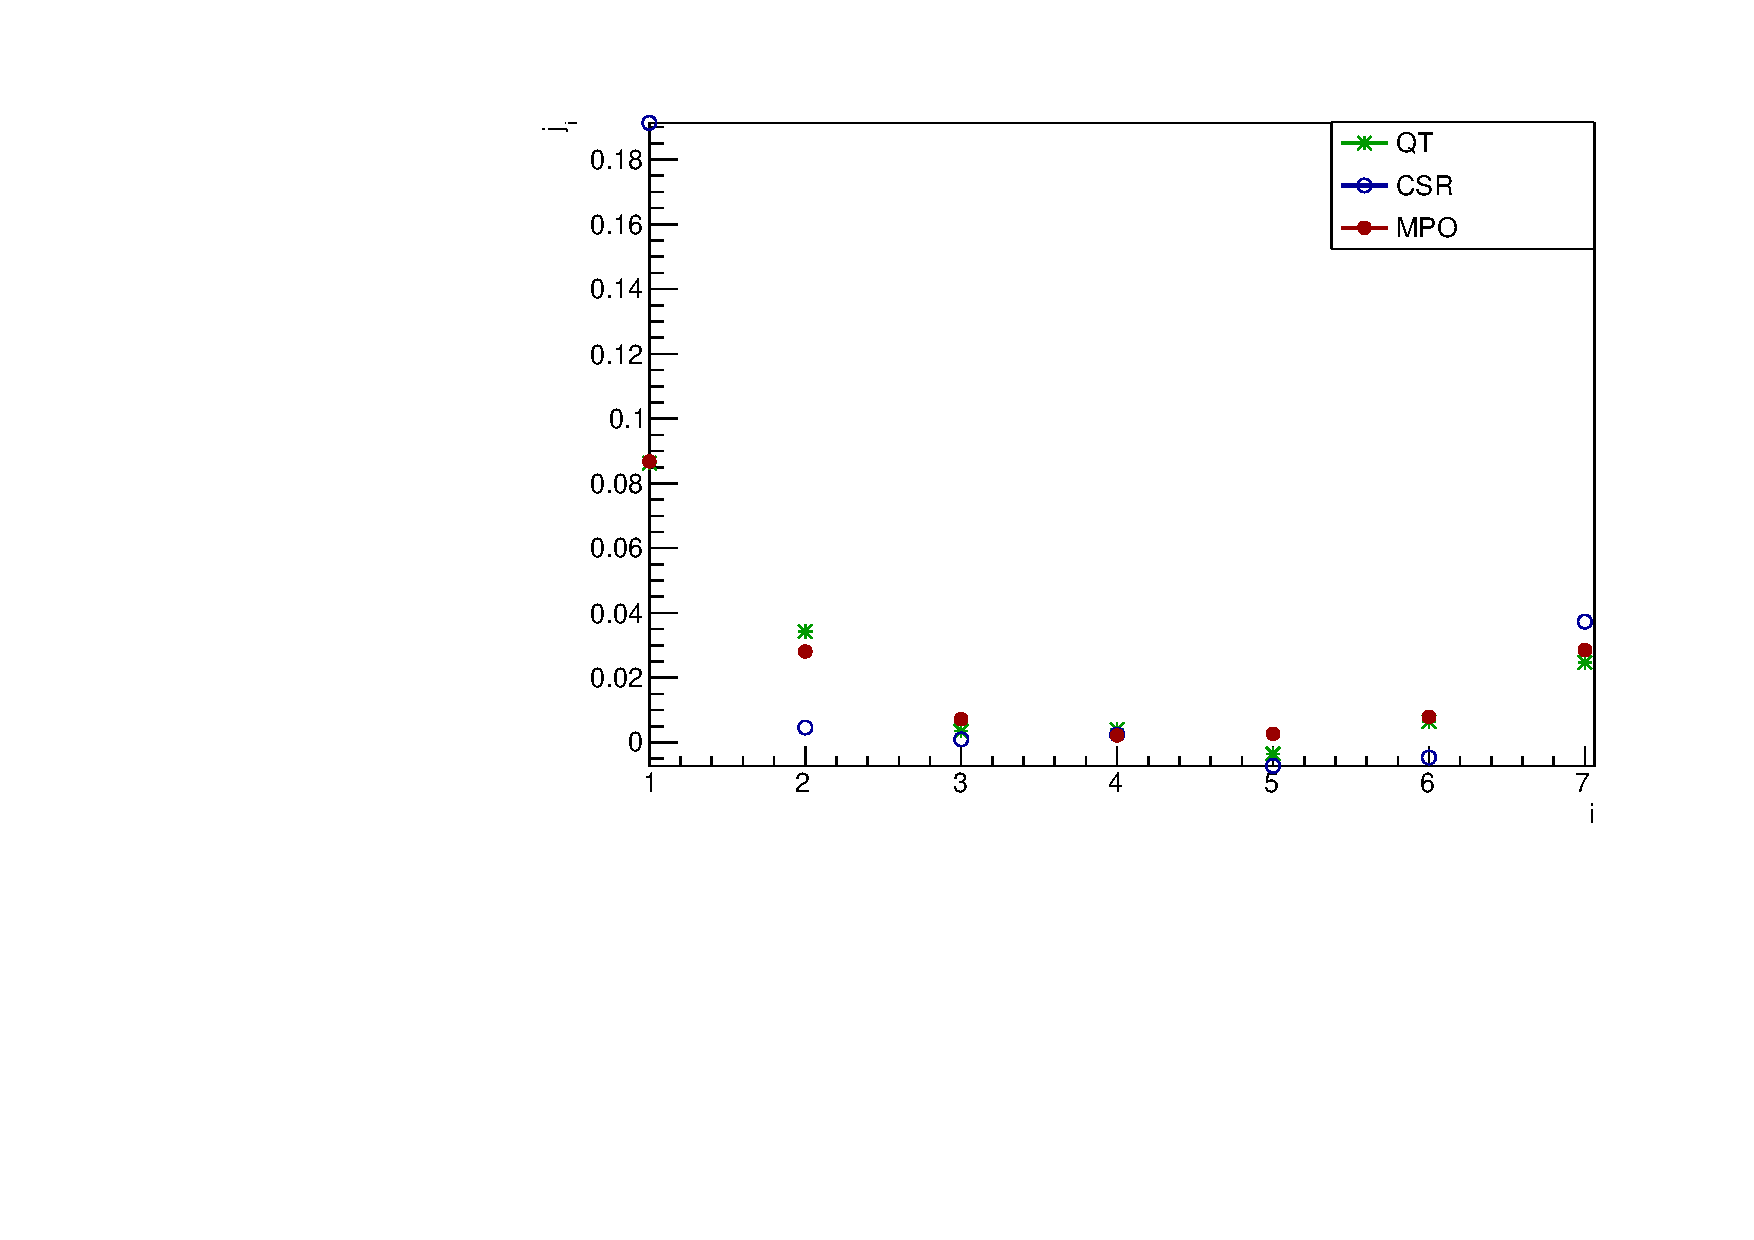
\includegraphics[scale=0.7]{Figures/8sites_comparison/SpinCurr_8s_J10515.pdf}
    \caption{Spin current of the chain, characterized by $\gamma=1, J_x=1, J_y=0.5, J_z=1.5$; \emph{i} stands for the site index.}
    \label{fig:my_label}
\end{figure}

Let us see what happens in the case of a \textbf{12-sites} chain.

\begin{figure}[H]
    \centering
    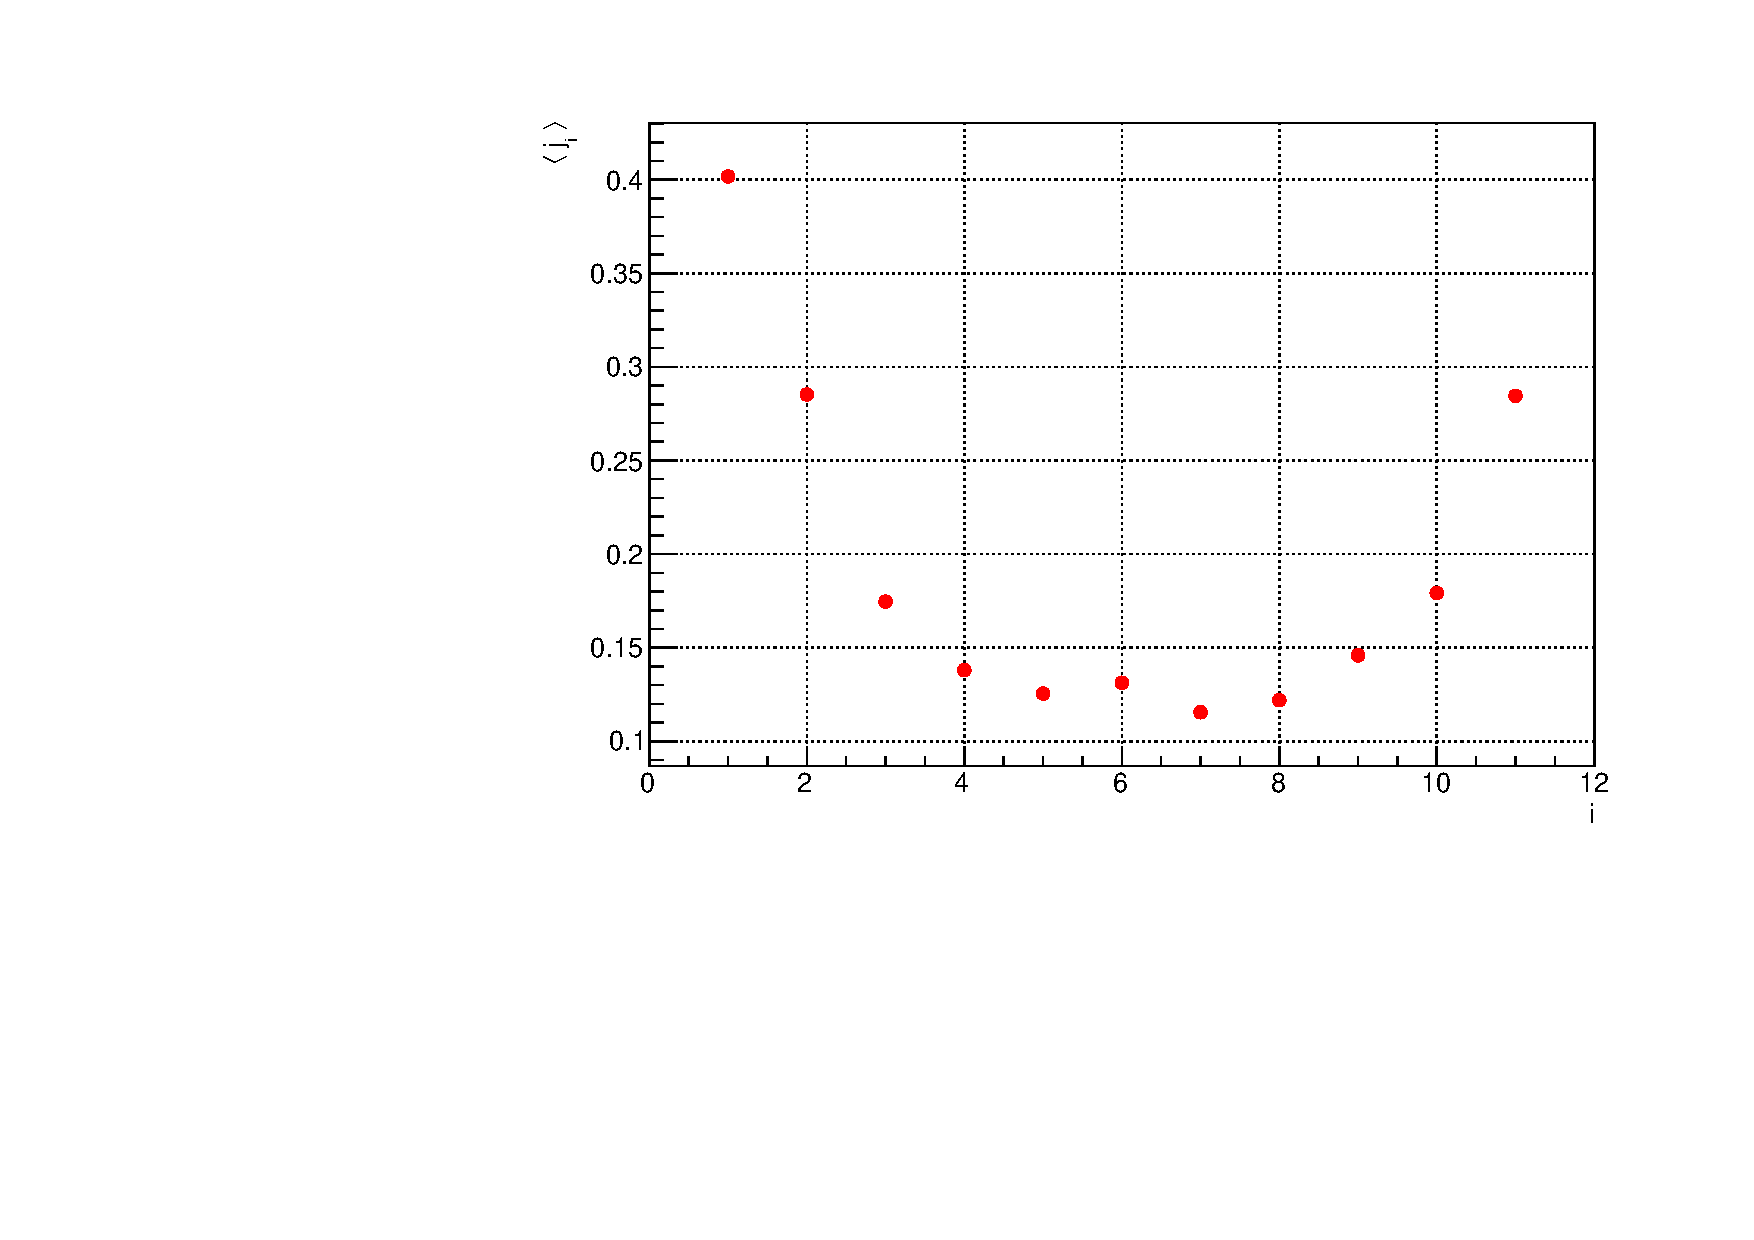
\includegraphics[scale=0.7]{Figures/12sites/SpinCurrL012m060Time002000_J10505.pdf}
    \caption{Spin current of a 12-sites chain, characterized by $\gamma=1, J_x=1, J_y=0.5, J_z=0.5$; \emph{i} stands for the site index. Data are obtained from MPO method.}
    \label{fig:my_label}
\end{figure}

\begin{figure}[H]
    \centering
    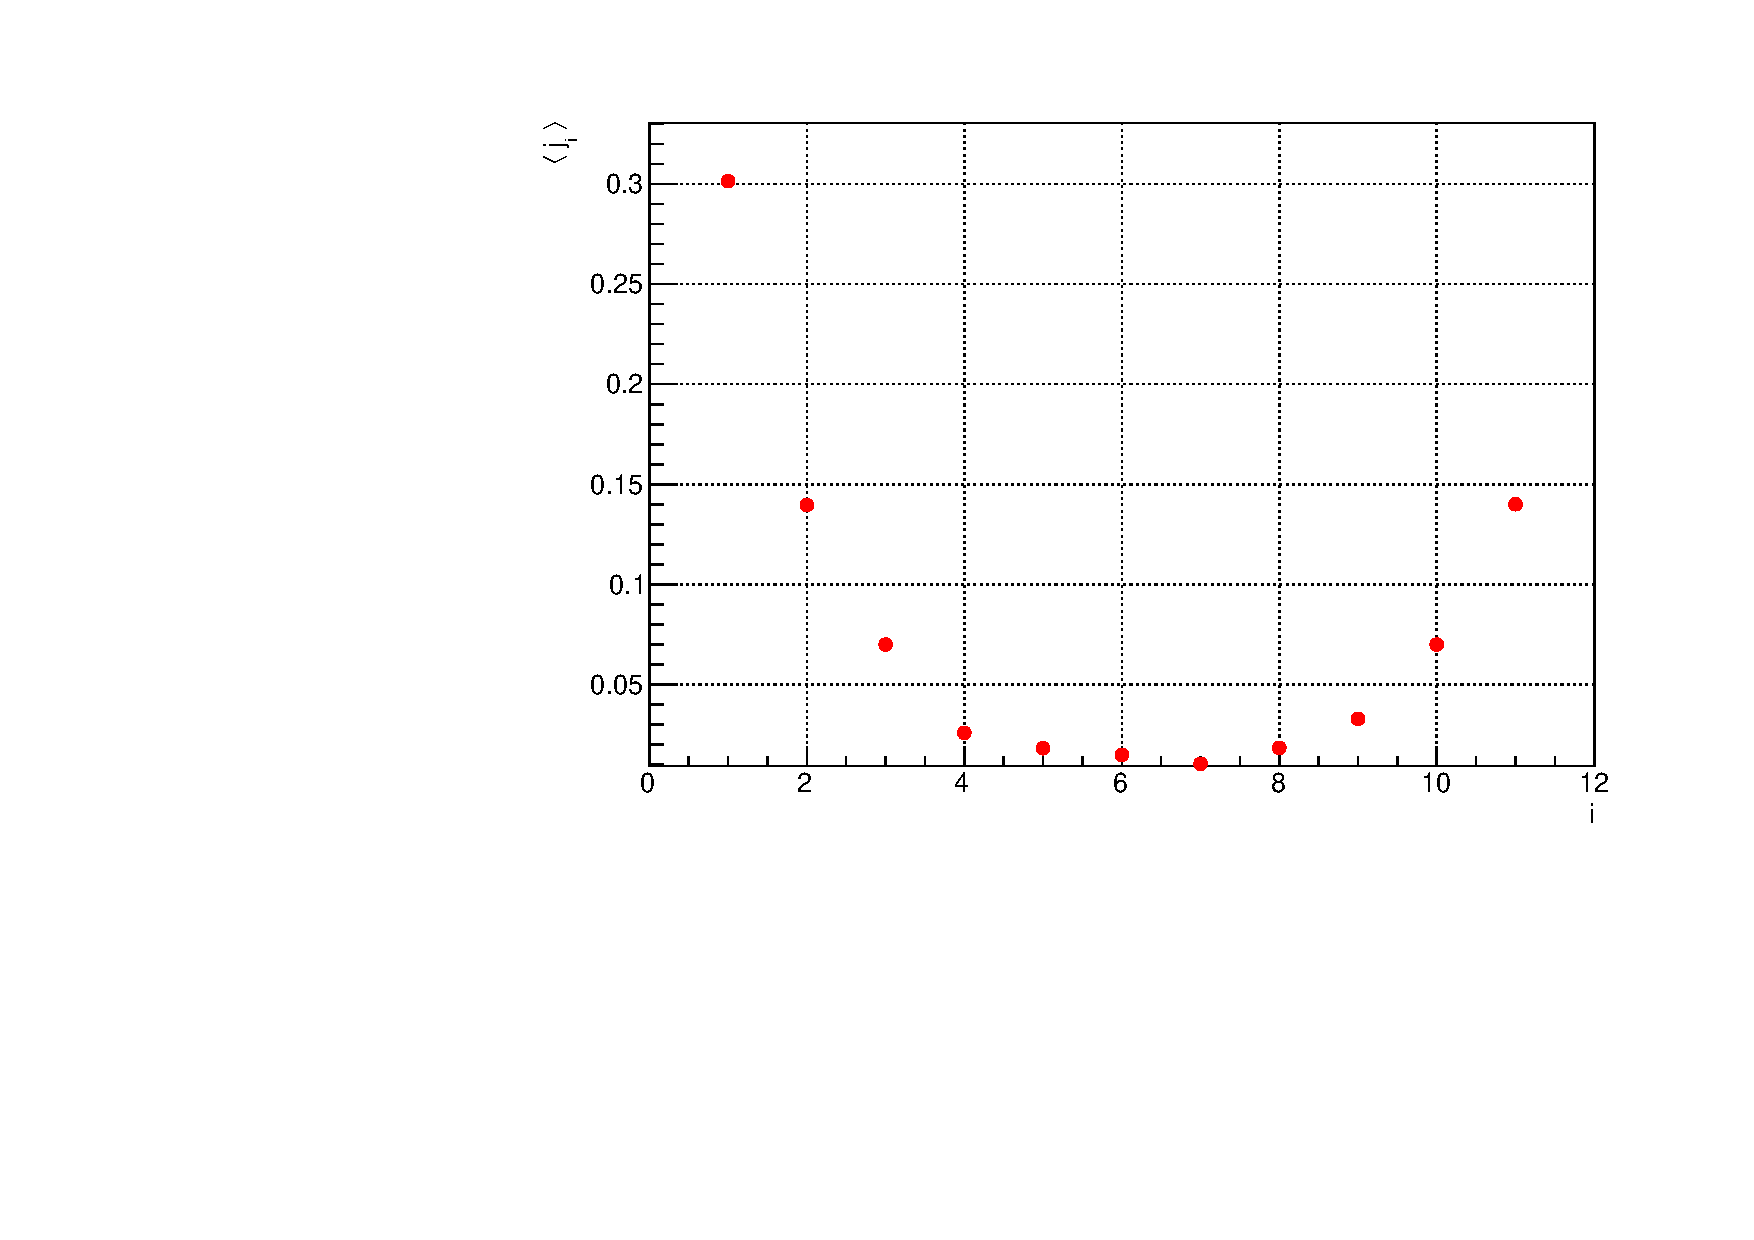
\includegraphics[scale=0.7]{Figures/12sites/SpinCurrL012m060Time002000_J1051.pdf}
    \caption{Spin current of a 12-sites chain, characterized by $\gamma=1, J_x=1, J_y=0.5, J_z=1.$; \emph{i} stands for the site index. Data are obtained from MPO method.}
    \label{fig:my_label}
\end{figure}

\begin{figure}[H]
    \centering
    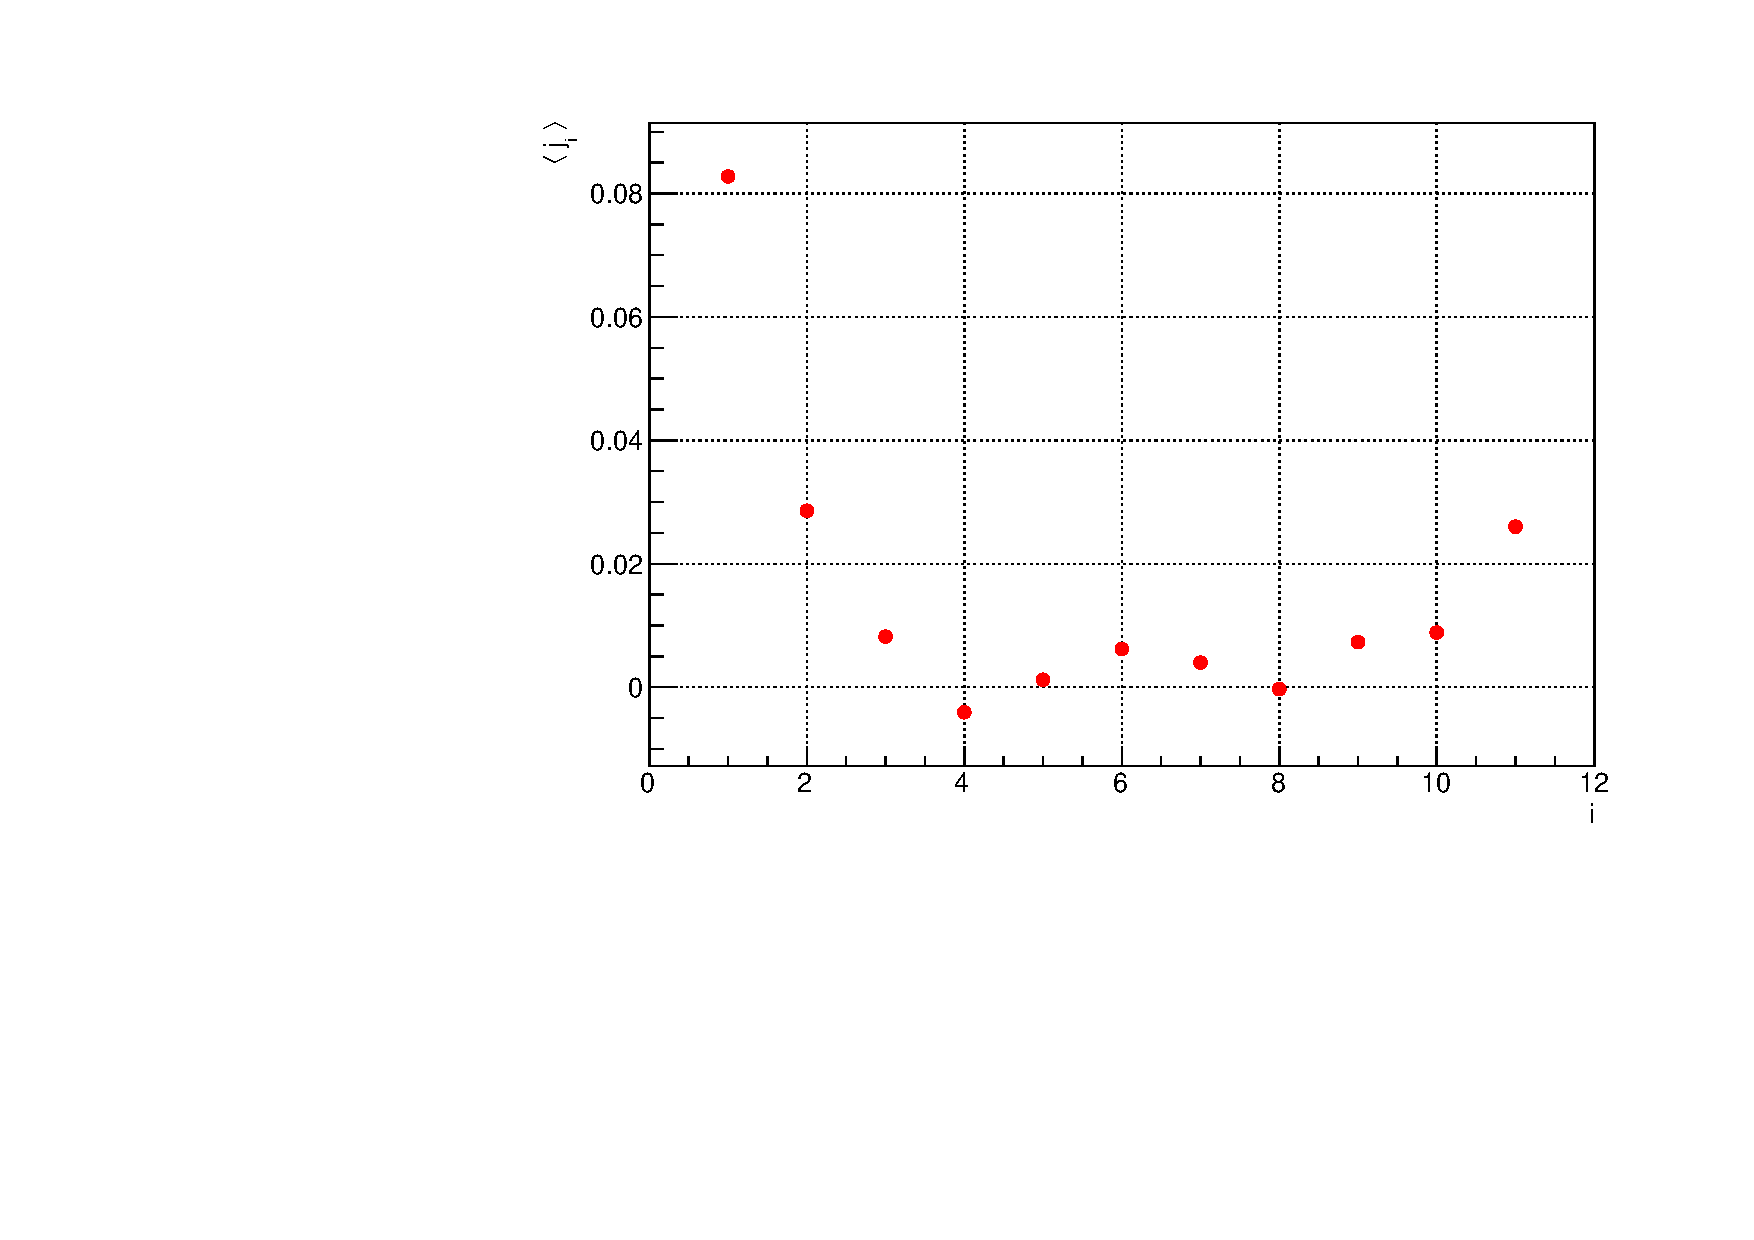
\includegraphics[scale=0.7]{Figures/12sites/SpinCurrL012m060Time002000_J10515.pdf}
    \caption{Spin current of a 12-sites chain, characterized by $\gamma=1, J_x=1, J_y=0.5, J_z=1.5$; \emph{i} stands for the site index. Data are obtained from MPO method.}
    \label{fig:my_label}
\end{figure}

\begin{figure}[H]
    \centering
    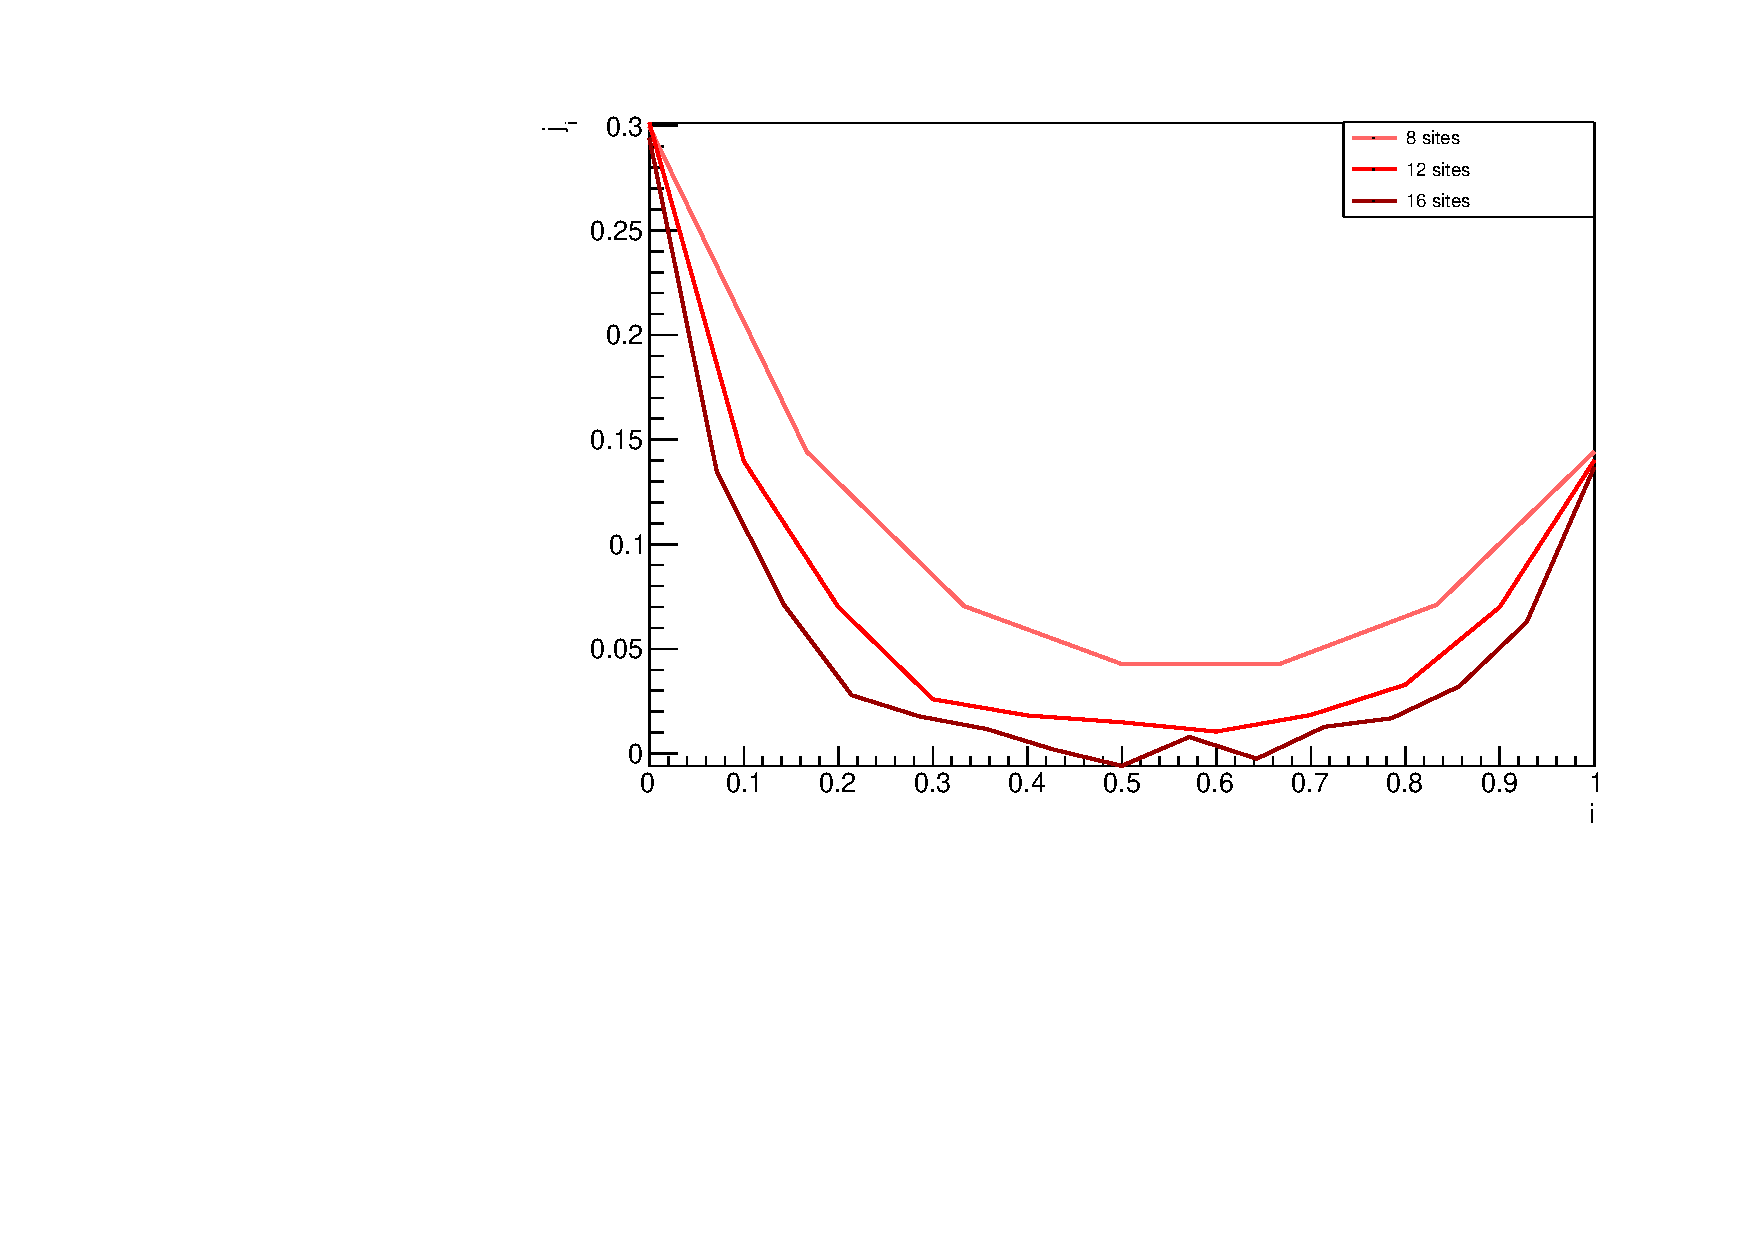
\includegraphics[scale=0.7]{Figures/NORM_SpinCurr_comparisonVSsize.pdf}
    \caption{Spin current for the model at $J_z = 1$. Data for different chain lengths are shown. They are obtained from MPO method.}
    \label{fig:my_label}
\end{figure}

\begin{figure}[H]
    \centering
    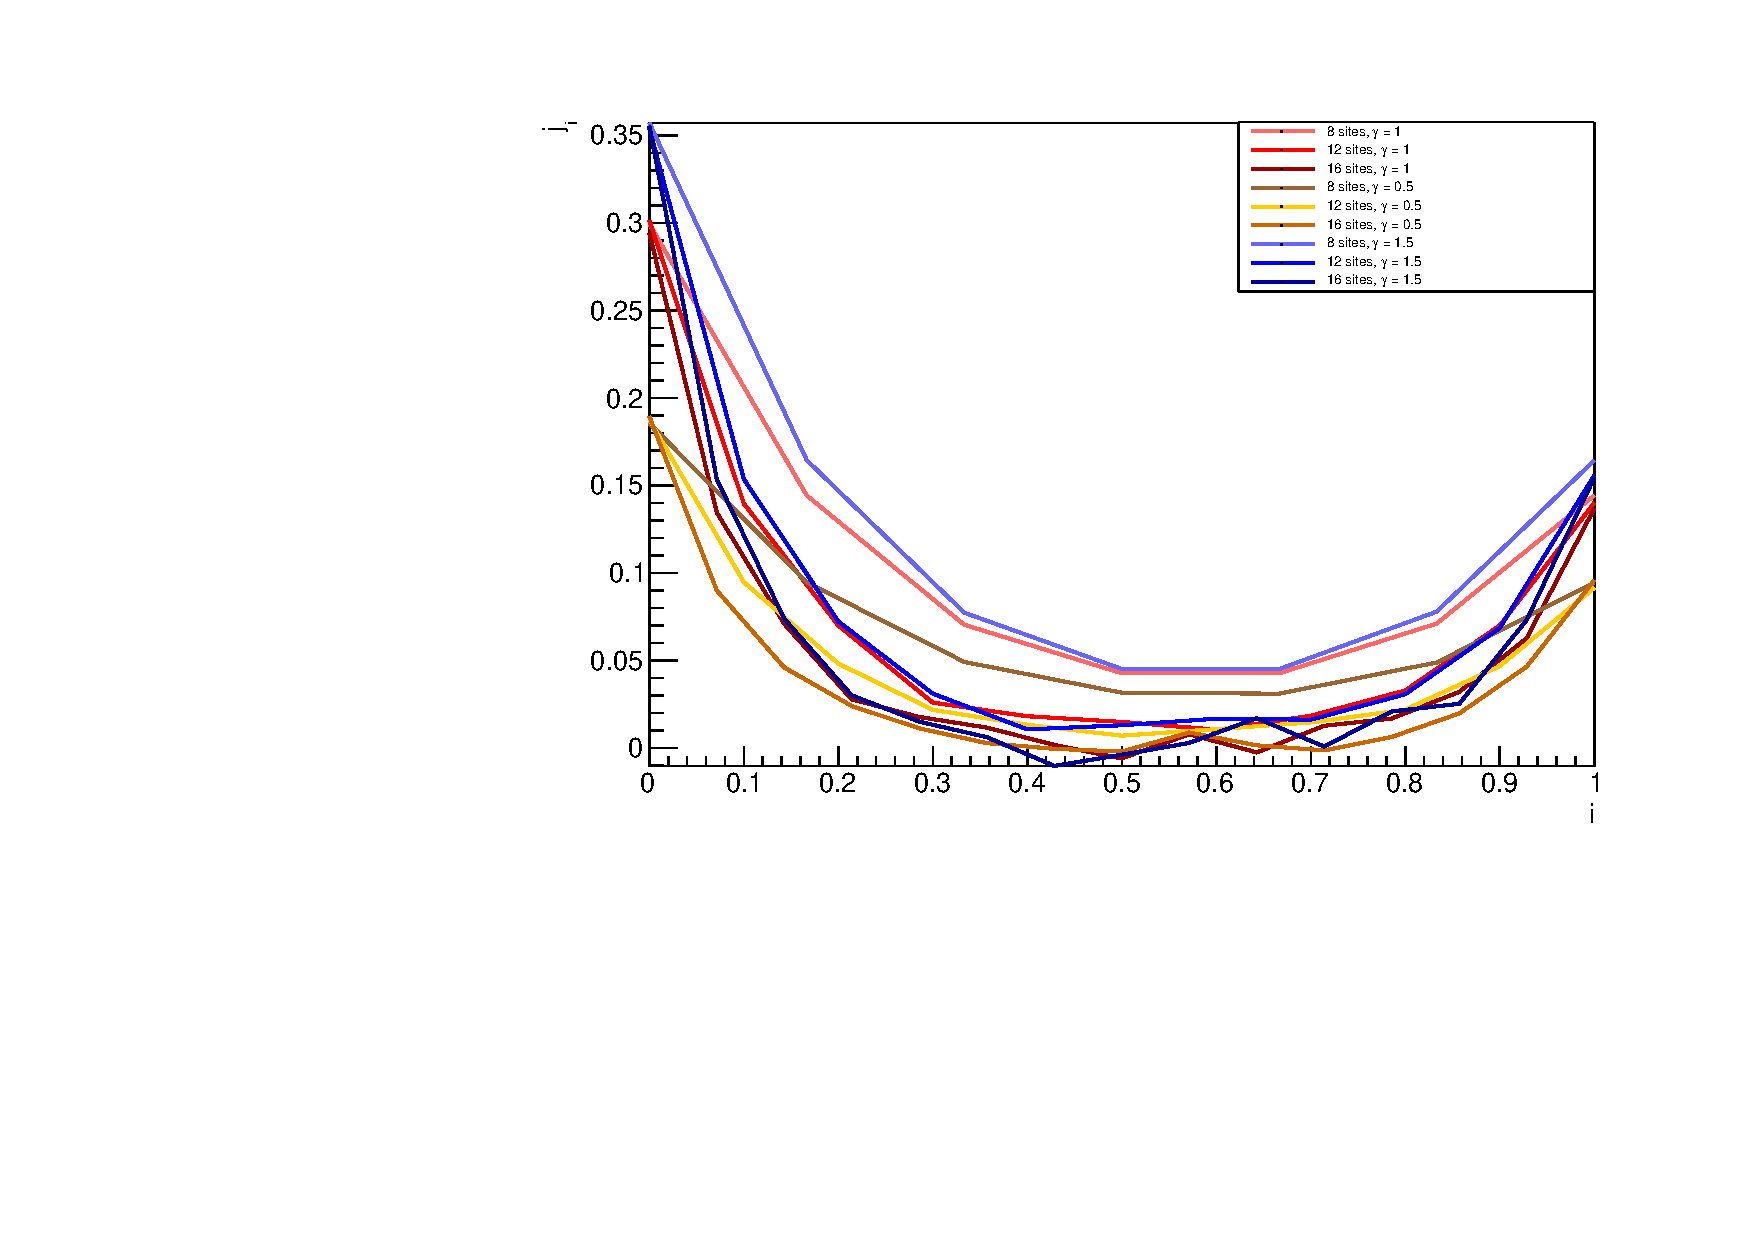
\includegraphics[scale=0.7]{Figures/SpinCurrcomparisonVSsizeANDdissipationRate.pdf}
    \caption{Caption}
    \label{fig:my_label}
\end{figure}